\documentclass[a4paper]{report}
\usepackage[spanish]{babel}
\usepackage{graphicx}
\pagestyle{headings}
\titlepage
\usepackage[utf8]{inputenc} % para codificacion unicode (utf8)
\usepackage{enumerate}
\usepackage{hyperref} % para links a paginas web
\usepackage{subfig}
\usepackage{graphics}
\usepackage{amsmath}
\usepackage{amssymb}
\usepackage{amsthm}
\usepackage{placeins}
\usepackage{tabularx}
\usepackage{booktabs,siunitx}
\usepackage{calc}
\usepackage{bm}
\usepackage{fullpage}
\usepackage{mathdots}
\usepackage{multirow}
\usepackage{polynom}

% plot a circle
\usepackage{tikz}
\newcommand\TikCircle[1][3]{\tikz[baseline=-#1]{\draw[thick](0,0.05)circle[radius=#1mm];}}


\decimalpoint

% That follow is for listings configuration
\usepackage{listings}
\usepackage{color}
\usepackage{textcomp}
\definecolor{listinggray}{gray}{0.9}
\definecolor{lbcolor}{rgb}{0.99,0.99,0.99}
\lstset{
    backgroundcolor=\color{lbcolor},
    tabsize=4,
    rulecolor=,
    language=python,
    basicstyle=\scriptsize,
    upquote=true,
    aboveskip={1.5\baselineskip},
    columns=fixed,
    showstringspaces=false,
    extendedchars=true,
    breaklines=true,
    prebreak = \raisebox{0ex}[0ex][0ex]{\ensuremath{\hookleftarrow}},
    frame=single,
    showtabs=false,
    showspaces=false,
    showstringspaces=false,
    identifierstyle=\ttfamily,
    keywordstyle=\color[rgb]{0,0,1},
    commentstyle=\color[rgb]{0.133,0.545,0.133},
    stringstyle=\color[rgb]{0.627,0.126,0.941},
    literate=%
        {á}{{\'{a}}}1
        {é}{{\'{e}}}1
        {í}{{\'{i}}}1
        {ó}{{\'{o}}}1
        {ú}{{\'{u}}}1
        {ñ}{{\~n}}1
}
\newcommand{\var}{\operatorname{var}}
\newcommand{\x}{\mathbf{x}}
\newcommand{\y}{\mathbf{y}}
\newcommand{\w}{\mathbf{w}}
\newcommand{\z}{\mathbf{z}}
\newcommand{\g}{\mathbf{g}}
\newcommand{\h}{\mathbf{h}}
\newcommand{\s}{\mathbf{s}}
\newcommand{\thetabf}{\bm{\theta}}
\newcommand{\alphabf}{\bm{\alpha}}
\newcommand{\mubf}{\bm{\mu}}
\newcommand{\I}{\mathbf{I}} % Fisher information matrix
\newcommand{\C}{\mathbf{C}} % Covariance matrix
\newcommand{\abf}{\mathbf{a}}
\newcommand{\bbf}{\mathbf{b}}
\newcommand{\e}{\mathbf{e}}
\newcommand{\ubf}{\mathbf{u}}
\newcommand{\vbf}{\mathbf{v}}
\newcommand{\A}{\mathbf{A}}
\newcommand{\B}{\mathbf{B}}
\newcommand{\D}{\mathbf{D}}
\newcommand{\G}{\mathbf{G}}
\newcommand{\Hbf}{\mathbf{H}}
\newcommand{\K}{\mathbf{K}}
\newcommand{\Lbf}{\mathbf{L}}
\newcommand{\M}{\mathbf{M}}
\newcommand{\R}{\mathbf{R}}
\newcommand{\T}{\mathbf{T}}
\newcommand{\W}{\mathbf{W}}
\newcommand{\X}{\mathbf{X}}
\newcommand{\Pbf}{\mathbf{P}}
\renewcommand{\Re}{\operatorname{Re}}
\renewcommand{\Im}{\operatorname{Im}}
\DeclareMathOperator*{\argmin}{arg\,min}
\DeclareMathOperator*{\argmax}{arg\,max}
\DeclareMathOperator{\PV}{P.V.}
\DeclareMathOperator{\tr}{tr}
\DeclareMathOperator{\cov}{cov}
\DeclareMathOperator{\ARG}{ARG}
\DeclareMathOperator{\Log}{Log}
\DeclareMathOperator{\sech}{sech}
\DeclareMathOperator{\csch}{csch}
\DeclareMathOperator{\grd}{grd}
\def\Res{\qopname\relax m{Res}}


\title{Estudiando el libro ``Discrete-Time Signal Processing''\\de Alan V. Oppenheim y Ronald W. Schafer}
\author{Ernesto López}


\begin{document} 

\hypersetup{pageanchor=false}
\maketitle
\hypersetup{pageanchor=true}
\pagenumbering{roman}
\tableofcontents


\chapter*{Prefacio}

El presente documento consiste en apuntes sobre procesamiento de señales discretas. Se seguirá fielmente el libro \cite{oppenheim2009discrete}. Solo se incluye un resumen de los conceptos básicos y se profundizará en los tópicos mas avanzados de procesamiento de señales incluidos en el libro.

\pagenumbering{arabic}

\chapter{Señales y sistemas en tiempo discreto}\label{ch:signals_and_systems}

\section{Señales en tiempo discreto}

En la teoría de señales y sistemas en tiempo discreto, hay secuencias son de particular importancia. Algunas son las siguientes:
\begin{itemize}
 \item \emph{Impuso unidad:}
 \begin{equation}\label{eq:seq_and_sys_unit_sample}
  \delta[n]=
  \left\{
  \begin{array}{rr}
   0, & n\neq0,\\
   1, & n=0.
  \end{array}
  \right.  
 \end{equation}
 Un aspecto importante del impuso unidad es que cualquier secuencia puede expresarse como la suma de impulsos desplazados y escalados como
 \begin{equation}\label{eq:seq_and_sys_sequence_as_impuses_sum}
  x[n]=\sum_{k=-\infty}^\infty x[k]\delta[n-k].  
 \end{equation}
 \item\emph{Escalón unidad:}
  \begin{equation}\label{eq:seq_and_sys_unit_step}
  u[n]=
  \left\{
  \begin{array}{rr}
   1, & n\geq0,\\
   0, & n<0.
  \end{array}
  \right.  
 \end{equation}
 El escalón unidad está relacionado con el impuso unidad por
 \[
  u[n]=\sum_{k=-\infty}^n\delta[k],
 \]
 es decir, el escalón unidad en el índice (tiempo) \(n\) es la suma acumulada de todas las muestras del impulso unidad hasta el tiempo \(n\). Una representación alternativa del escalón unidad en términos de impulsos es 
 \[
  u[n]=\sum_{k=0}^\infty\delta[n-k],
 \]
 como en la ecuación \ref{eq:seq_and_sys_sequence_as_impuses_sum}. Por otro lado, el impuso puede expresarse como  la \emph{primera diferencia regresiva} del escalón unidad, es decir,
 \[
  \delta[n]=u[n]-u[n-1].
 \]
 \item\emph{Exponencial:}
 \begin{equation}\label{eq:seq_and_sys_exponential}
  u[n]=A\alpha^n,
 \end{equation}
 donde en el caso mas general, \(\alpha\) y \(A\) son números complejos. Específicamente, si \(\alpha=|\alpha|e^{j\omega_0}\) y \(A=|A|e^{j\phi}\),
 \begin{align*}
  x[n]&=|A||\alpha|^ne^{j(\omega_0n+\phi)}\\
   &=|A||\alpha|^n\cos(\omega_0n+\phi)+j|A||\alpha|^n\sen(\omega_0n+\phi).  
 \end{align*}
 
 Si \(|\alpha|=1\), la secuencia toma la forma
 \begin{align*}
  x[n]&=|A|e^{j(\omega_0n+\phi)}\\
   &=|A|\cos(\omega_0n+\phi)+j|A|\sen(\omega_0n+\phi). 
 \end{align*}
 En esta secuencia, la parte real e imaginaria oscilan sinusoidalmente con \(n\). Por analogía con el caso en tiempo continuo, \(\omega_0\) es la \emph{frecuencia} y \(\phi\) es la \emph{fase}. Sin embargo, como \(n\) es adimensionado, las unidades de \(\omega_0\) son radianes. Para mantener un analogía mas cercana al caso continuo, puede especificarse que las unidades de \(\omega_0\) son radianes por muestra y las unidades de \(n\) son muestras.
 
 El hecho de que \(n\) sea un número entero conduce a diferencias importantes de las propiedades de las señales exponenciales complejas y sinusoidales en tiempo continuo y en tiempo discreto. A diferencia del caso en tiempo continuo, las secuencias exponenciales complejas y sinusoidales con frecuencias \(\omega_0+2\pi r\), con \(r\) entero, son indistinguibles entre si, ya que 
 \[
  e^{j[(\omega_0+2\pi r)n+\phi]}=e^{j(\omega_0n+\phi)}.
 \]
 Por lo tanto, al estudiar secuencias exponenciales complejas de la forma \(x[n]=Ae^{j(\omega_0n+\phi)}\) o señales sinusoidales reales de la forma \(x[n]=A\cos(\omega_0n+\phi)\) solo se necesita considerar frecuencias en un intervalo de \(2\pi\). Típicamente se eligen los intervalos \(-\pi<\omega_0\leq\pi\) o \(0\leq\omega_0<2\pi\).

 A diferencia del caso en tiempo continuo, una secuencia exponencial compleja o sinusoidal no necesariamente es periódica. Las secuencias periódicas son aquellas que cumplen que 
 \[
  x[n]=x[n+N],
  \qquad\qquad\textrm{para todo }n,
 \]
 donde el período \(N\) es entero. Si se prueba está condición para una secuencia sinusoidal,
 \[
  A\cos(\omega_0n+\phi)=A\cos(\omega_0n+\omega_0N+\phi),
 \]
 se requiere que
 \begin{equation}\label{eq:seq_and_sys_sinusoidal_periodicity_condition}
  \omega_0N=2\pi k,  
 \end{equation}
 con \(k\) entero. Por lo tanto, las secuencias exponenciales complejas y sinusoidales no necesariamente son periódicas con período \(2\pi/\omega_0\), y dependiendo del valor de \(\omega_0\), pueden no ser periódicas en absoluto.
 
 Si se combina la condición de la ecuación \ref{eq:seq_and_sys_sinusoidal_periodicity_condition} con la observación previa de que las frecuencias \(\omega_0\) y \(\omega_0+2\pi r\) son indistinguibles, se deduce que una secuencia de período \(N\) puede ser de \(N\) frecuencias distinguibles. El conjunto de frecuencias distintas es
 \[
  \omega_k=\frac{2\pi k}{N},
  \qquad\qquad
  k=0,\,1,\,\dots,\,N-1. 
 \]
 
 Vinculado a la discusión precedente es el hecho de que la interpretación de bajas y altas frecuencias es distinto para secuencias exponenciales complejas y sinusoidales. Para la secuencia sinusoidal \(x[n]=A\cos(\omega_0n+\phi)\), cuando la frecuencia \(\omega_0\) crece desde \(\omega_0=0\) a \(\omega_0=\pi\), \(x[n]\) oscila progresivamente mas rápidamente, pero cuando la frecuencia \(\omega_0\) crece desde \(\omega_0=\pi\) a \(\omega_0=2\pi\), las oscilaciones se hacen mas lentas. Esto es porque las frecuencias \(\omega_0\) y \(2\pi-\omega_0\) tienen la misma velocidad de oscilación, ya que, por ejemplo
 \[
  \sen[(2\pi-\omega_0)n]=\sen(2\pi n-\omega_0n)=\sen(-\omega_0n)=-\sen(\omega_0n).
 \]
 Como consecuencia, para secuencias sinusoidales y exponenciales complejas, las frecuencias cercanas a \(\omega_0=2\pi k\), con \(k\) entero, son referidas como bajas frecuencias, y las frecuencias en la vecindad de \(\pi+2\pi k\), con \(k\) entero, son referidas como altas frecuencias.
\end{itemize} 
 
\section{Sistemas en tiempo discreto}

Un sistema en tiempo discreto se define matemáticamente como una transformación que se aplica sobre una secuencia de entrada \(x[n]\) para obtener una secuencia de salida \(y[n]\). Se denota como
\[
 y[n]=T\{x[n]\}.
\]

A continuación se dan ejemplos de algunos sistemas básicos que serán útiles para ilustrar las propiedades de los sistemas en tiempo discreto mas adelante.
\begin{itemize}
 \item\emph{Retardo ideal:}
 \begin{equation}\label{eq:seq_and_sys_system_ideal_delay}
  y[n]=x[n-n_d],
  \qquad\qquad
  -\infty<n<\infty,  
 \end{equation}
 donde \(n_d\) es un entero positivo. El retardo ideal desplaza la entrada hacia la derecha \(n_d\) muestras. En el caso en que \(n_d\) es negativo, desplaza la señal de entrada a la izquierda \(n_d\) muestras, correspondiendo a un adelanto temporal.
 \item\emph{Media móvil:} 
 \begin{equation}\label{eq:seq_and_sys_system_moving_average}
  y[n]=\frac{1}{M_1+M_2+1}\sum_{k=-M_1}^{M_2}x[n-k].  
 \end{equation}
 En este sistema, la \(n\)-ésima nuestra de la salida es el promedio de \(M_1+M_2+1\) muestras de la entrada en torno a la \(n\)-ésima muestra.
 \item\emph{Acumulador:} 
 \begin{equation}\label{eq:seq_and_sys_system_accumulator}
  y[n]=\sum_{k=-\infty}^nx[k].   
 \end{equation}
 Las salida en el tiempo \(n\) es la suma de la muestra presente y todas las muestras pasadas de la entrada.
 \item\emph{Compresor:}
 \begin{equation}\label{eq:seq_and_sys_system_compressor}
  y[n]=x[Mn],
  \qquad\qquad 
  -\infty<n<\infty,  
 \end{equation}
 donde \(M\) es un entero positivo. Este sistema descarta \(M-1\) por cada \(M\) muestras de la entrada.
 \item\emph{Diferencia progresiva y regresiva:} el sistema diferencia progresiva esta dado por la ecuación
 \begin{equation}\label{eq:seq_and_sys_system_forward_difference}
  y[n]=x[n+1]-x[n]
 \end{equation}
 y el sistema diferencia regresiva esta dado por la ecuación
  \begin{equation}\label{eq:seq_and_sys_system_backward_difference}
  y[n]=x[n]-x[n-1].
 \end{equation}
\end{itemize}

Imponiendo restricciones sobre las propiedades de la transformación \(T\{\cdot\}\) se definen clases de sistemas. En las siguientes secciones se brinda una clasificación de sistemas con restricciones y propiedades especialmente importantes. 

\subsection{Sistemas sin memoria}
 
Un sistema se dice sin memoria si la salida \(y[n]\) en cada instante \(n\) depende solo de la entrada \(x[n]\) en el mismo instante \(n\). 

Los sistemas retardo ideal y media móvil no son sin memoria a menos que \(n_d=0\) y \(M_1=M_2=0\) respectivamente. El resto de los sistemas definidos al comienzo de la sección también son sin memoria. Un ejemplo de un sistema sin memoria es
\begin{equation}\label{eq:seq_and_sys_system_input_square}
 y[n]=(x[n])^2. 
\end{equation}

\subsection{Sistemas lineales}

La clase de sistemas lineales está definida por el \emph{principio de superposición}. Si \(y_1[n]\) e \(y_2[n]\) son las respuestas de un sistema cuando las entradas son \(x_1[n]\) y \(x_2[n]\) respectivamente, el sistema es lineal si y solo si
\begin{equation}\label{eq:seq_and_sys_sys_properties_superposition}
 T\{ax_1[n]+bx_2[n]\}=aT\{x_1[n]\}+bT\{x_2[n]\}, 
\end{equation}
donde \(a\) y \(b\) son constantes arbitrarias. La ecuación \ref{eq:seq_and_sys_sys_properties_superposition} es el principio de superposición.

La prueba de que un sistema es lineal requiere una demostración general sin realizar hipótesis específicas sobre las señales de entrada. Por el contrario, la prueba de que un sistema no es lineal solo requiere un contraejemplo. 

A partir del principio de superposición puede mostrarse que todos los sistemas presentados al comienzo de esta sección son lineales. El sistema definido por la ecuación \ref{eq:seq_and_sys_system_input_square} no es lineal.

\subsection{Sistemas invariantes en el tiempo} 
 
Un sistema invariante en el  tiempo es un sistema para el cual un desplazamiento temporal de la secuencia de entrada produce el mismo desplazamiento temporal en la secuencia de salida. Específicamente, supóngase que un sistema transforma la secuencia de entrada \(x[n]\) en la secuencia de salida \(y[n]\). El sistema es invariante en el tiempo si, para todo \(n_0\), la secuencia de entrada \(x_1[n]=x[n-n_0]\) produce la secuencia de salida \(y_1[n]=y[n-n_0]\). 

Al igual que con los sistemas lineales, la prueba de la invarianza temporal requiere una demostración general sin imposición de hipótesis sobre la secuencia de entrada, y alcanza un contraejemplo para probar lo contrario.

El sistema compresor, dado por la ecuación \ref{eq:seq_and_sys_system_compressor}, no es invariante en el tiempo. Si lo fuera, dado que la entrada \(x[n]\) produce la salida \(y[n]=x[Mn]\), la entrada \(x_1[n]=x[n-n_0]\) debería producir la salida
\[
 y[n-n_0]=x[M(n-n_0)]=x[Mn-Mn_0].
\]
Sin embargo, la entrada \(x_1[n]\) produce la salida
\[
 y_1[n]=x_1[Mn]=x[Mn-n_0],
\]
que es distinta a \(y[n-n_0]\). La no invarianza también se podría mostrar con un contraejemplo: sea \(M=2\), \(x[n]=\delta[n]\) y \(n_0=1\), es decir, \(x_1[n]=x[n-1]=\delta[n-1]\). La salida es \(y[n]=\delta[n]\), pero \(y_1[n]=0\), y por lo tanto, como \(y[n-1]\neq y_1[n]\), el sistema no es invariante en el tiempo. Puede probarse que el resto de los sistemas al comienzo de la sección son invariantes en el tiempo.

\subsection{Sistemas causales}\label{sec:seq_and_sys_causal_system} 

Un sistema es causal si para cada \(n_0\), la secuencia de salida en el instante \(n=n_0\) depende solo de valores de la secuencia de entrada en \(n\leq n_0\). Esto implica que si \(x_1[n]=x_2[n]\) para \(n\leq n_0\) se cumple que \(y_1[n]=y_2[n]\) para \(n\leq n_0\). Conceptualmente significa que el sistema es \emph{no anticipativo}.

Para verificar si el sistema retardo ideal es causal, sean las entradas \(x_1[n]\) y \(x_2[n]\) que cumplen que \(x_1[n]=x_2[n]\) para \(n\leq n_0\), y sean \(y_1[n]=x_1[n-n_d]\) y \(y_2[n]=x_2[n-n_d]\) las salidas correspondientes. De esta forma, \(y_1[n]=y_2[n]\) si \(x_1[n-n_d]=x_2[n-n_d]\), y por hipótesis esto es cierto si 
\begin{equation}\label{eq:seq_and_sys_causality_proof_tmp}
 n-n_d\leq n_0
 \qquad\qquad\Leftrightarrow\qquad\qquad 
 n\leq n_0+n_d. 
\end{equation}
Pero para que el sistema sea causal se requiere que \(y_1[n]=y_2[n]\) para \(n\leq n_0\), lo que en la condición \ref{eq:seq_and_sys_causality_proof_tmp} ocurre si \(n_d\geq0\). Se concluye que el sistema es causal si \(n_d\geq0\) y no es causal si \(n_d<0\). En general, en la práctica es directo determinar si un sistema es causal inspeccionando si en la ecuación del sistema la salida depende de muestras futuras de la entrada. Así, el sistema media móvil de la ecuación \ref{eq:seq_and_sys_system_moving_average} es causal si \(M_1\leq0\) y \(M_2\geq0\), y en otro caso es no causal. El sistema acumulador y el sistema diferencia regresiva de las ecuaciones \ref{eq:seq_and_sys_system_accumulator} y \ref{eq:seq_and_sys_system_backward_difference} son causales. El sistema compresor de la ecuación \ref{eq:seq_and_sys_system_compressor} no es causal si \(M>1\) y el sistema diferencia progresiva dado por la ecuación \ref{eq:seq_and_sys_system_forward_difference} no es causal.

\subsection{Sistemas estables}\label{sec:seq_and_sys_stable_system}

Un sistema es estable en el sentido \emph{entrada acotada, salida acotada} (\emph{BIBO}, Bounded Input, Bounded Output) si y solo si cada entrada acotada produce una salida acotada. La entrada es acotada si existe un número positivo fijo \(B_x\) tal que 
\[
 |x[n]|\leq B_x<\infty,
 \qquad\qquad\textrm{para todo } n.
\]
La propiedad de estabilidad requiere que para toda entrada acotada exista un número positivo fijo \(B_y\) tal que 
\[
 |y[n]|\leq B_y<\infty,
 \qquad\qquad\textrm{para todo } n.
\]

Puede probarse que los sistemas retardo ideal, media móvil y diferencia progresiva y regresiva son estables y el sistema acumulador no es estable.
 
\section{Sistemas lineales e invariantes en el tiempo} 
 
Una clase importante de sistemas son aquellos que son tanto lineales como invariantes en el tiempo (\emph{LTI}, Linear Time Invariant). La importancia radica en que conociendo la respuesta al impuso del sistema, es posible calcular la respuesta a cualquier entrada, y por lo tanto, tienen una gran cantidad de aplicaciones en procesamiento de señales. Específicamente, si \(h[n]\) es la respuesta al impulso de un sistema LTI, la salida es
\begin{equation}\label{eq:seq_and_sys_convolution_definition}
 y[n]=\sum_{k=-\infty}^\infty x[k]h[n-k],
 \qquad\qquad\textrm{para todo }n.
\end{equation}
Esta ecuación se denomina \emph{suma de convolución} y se representa mediante la notación
\[
 y[n]=x[n]*h[n].
\]

\section{Propiedades de los sistemas lineales e invariantes en el tiempo}\label{sec:seq_and_sys_lti_properties}  
 
Como el comportamiento de todos los sistemas LTI está determinado por la suma de convolución, las propiedades de esta clase de sistemas están establecidas por las propiedades de la convolución.  
 
Algunas propiedades generales de la convolución son las siguientes:
\begin{itemize}
 \item \emph{Conmutativa:}
 \[
  x[n]*h[n]=h[n]*x[n].
 \]
 Esto implica que un sistema LTI con entrada \(x[n]\) y respuesta al impulso \(h[n]\) tiene la misma salida que un sistema LTI con entrada \(h[n]\) y respuesta al impulso \(x[n]\), como se ilustra en la figura \ref{fig:lti_properties_conmutative}.
 \begin{figure}[!htb]
  \begin{minipage}[c]{0.53\textwidth}
    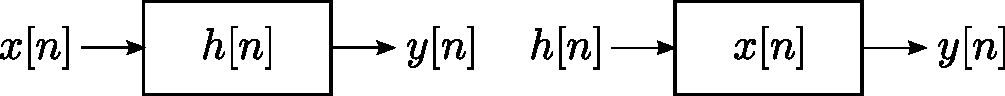
\includegraphics[width=\textwidth]{figuras/lti_properties_conmutative.pdf}
  \end{minipage}\hfill
  \begin{minipage}[c]{0.38\textwidth}
    \caption{
     Propiedad conmutativa de la convolución.
    }\label{fig:lti_properties_conmutative}
  \end{minipage}
\end{figure}
 \item \emph{Distributiva sobre la adición:}
 \[
  x[n]*(h_1[n]+h_2[n])=x[n]*h_1[n]+x[n]*h_2[n].
 \]
 Esto significa que el sistema equivalente a dos sistemas LTI en paralelo con respuestas al impulso \(h_1[n]\) y \(h_2[n]\) es un sistema LTI con respuesta al impulso \(h_1[n]+h_2[n]\), como se muestra en la figura \ref{fig:lti_properties_distributive}.
  \begin{figure}[!htb]
  \begin{minipage}[c]{0.6\textwidth}
    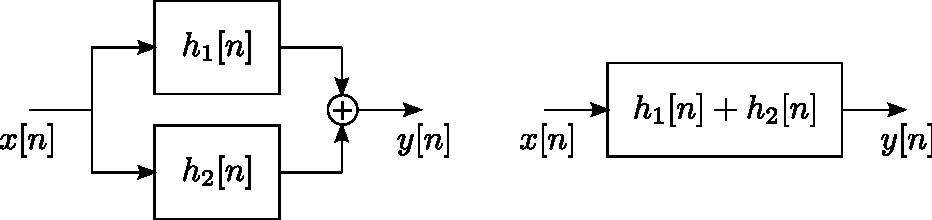
\includegraphics[width=\textwidth]{figuras/lti_properties_distributive.pdf}
  \end{minipage}\hfill
  \begin{minipage}[c]{0.3\textwidth}
    \caption{
     Propiedad conmutativa de la convolución y equivalencia de sistemas en paralelo.
    }\label{fig:lti_properties_distributive}
  \end{minipage}
 \end{figure}
 \item \emph{Asociativa:}
 \[
  y[n]=(x[n]*h_1[n])*h_2[n]=x[n]*(h_1[n])*h_2[n].
 \]
 Esto implica que la respuesta al impulso de dos sistemas LTI en serie es la convolución de sus respuestas al impulso, como se muestra en la figura \ref{fig:lti_properties_asociative}.
 \begin{figure}[!htb]
  \begin{minipage}[c]{0.65\textwidth}
    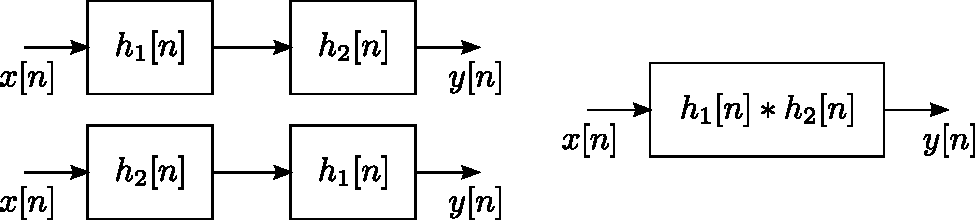
\includegraphics[width=\textwidth]{figuras/lti_properties_asociative.pdf}
  \end{minipage}\hfill
  \begin{minipage}[c]{0.25\textwidth}
    \caption{
     Propiedad asociativa de la convolución y equivalencia de sistemas en serie. 
    }\label{fig:lti_properties_asociative}
  \end{minipage}
 \end{figure}
\end{itemize}

Dos propiedades de los sistemas adicionales a la linealidad y la invarianza temporal son la estabilidad y la causalidad, y es importante poder determinar cuando un sistema LTI es estable y cuando es causal. Como los sistemas LTI están caracterizados por la respuesta al impulso, es posible determinar las propiedades del sistema a partir de las características de la respuesta al impulso.

\subsection{Estabilidad de los sistemas LTI}  
 
Recordar de la sección \ref{sec:seq_and_sys_stable_system} que un sistema es estable si toda entrada acotada produce una salida acotada. Puede mostrarse que un sistema LTI es estable si y solo si su respuesta al impulso es absolutamente sumable, es decir, si
\begin{equation}\label{eq:seq_and_sys_stability_condition}
 B_h=\sum_{k=-\infty}^\infty|h[k]|\leq\infty. 
\end{equation}

Para estudiar la estabilidad de un sistema, alcanza con calcular la respuesta al impulso a partir de la ecuación del sistema imponiendo como entrada \(\delta[n]\) y luego verificar si se cumple la ecuación \ref{eq:seq_and_sys_stability_condition}.

Por ejemplo, la respuesta al impulso de los sistemas media móvil y acumulador, dados respectivamente por las \ref{eq:seq_and_sys_system_moving_average} y \ref{eq:seq_and_sys_system_accumulator} son
\begin{itemize}
 \item \emph{Media móvil:}
 \begin{align}
  h[n]&=\frac{1}{M_1+M_2+1}\sum_{k=-M_1}^{M_2}\delta[n-k]\nonumber\\
   &=\frac{1}{M_1+M_2+1}\left(\delta[n+M_1]+\delta[n+M_1-1]+\cdots+\delta[n]+\cdots+\delta[n-M_2+1]+\delta[n-M_2]\right)\nonumber\\
   &=\left\{
   \begin{array}{ll}
    \dfrac{1}{M_1+M_2+1}, & -M_1\leq n\leq M_2\\
    0, &\textrm{en otro caso}.
   \end{array}
   \right.\nonumber\\
   &=\frac{1}{M_1+M_2+1}(u[n+M_1]-u[n-M_2-1])\label{eq:seq_and_sys_system_moving_average_impulse}
 \end{align}
 Por lo tanto,
 \[
  B_h=\sum_{k=-M_1}^{M_2}\frac{1}{M_1+M_2+1}=1,
 \]
 concluyendo que el sistema media móvil es estable.
 \item \emph{Acumulador:}
 \begin{align*}
  h[n]&=\sum_{k=-\infty}^n\delta[k]\\
   &=\left\{
   \begin{array}{ll}
    1, & n\geq0\\
    0, & n<0
   \end{array}
   \right.\\
   &=u[n].
 \end{align*}
 Por lo tanto,
 \[
  B_h=\sum_{k=-\infty}^\infty u[k]=\sum_{k=0}^\infty 1=\infty,
 \]
 concluyendo que el sistema acumulador no es estable.
\end{itemize}
Además, los sistemas retardo ideal y diferencia progresiva y regresiva, dados por las ecuaciones \ref{eq:seq_and_sys_system_ideal_delay}, \ref{eq:seq_and_sys_system_forward_difference} y \ref{eq:seq_and_sys_system_backward_difference} respectivamente, son estables. En general, un sistema con respuesta al impulso de duración finita (\emph{FIR}, finite-duration impulse response) es siempre estable si las muestras de la respuesta al impulso tienen magnitud finita. Observar que la respuesta al impulso del sistema acumular es de duración infinita (\emph{IIR}, infinite-duration impulse response).

\subsection{Causalidad de los sistemas LTI} 
 
Puede mostrarse a partir de la definición \ref{eq:seq_and_sys_convolution_definition} de la convolución que la condición necesaria y suficiente para que un sistema sea causal es que la respuesta al impulso cumpla que 
\begin{equation}\label{eq:seq_and_sys_causality_condition}
 h[n]=0,
 \qquad\qquad
 n<0. 
\end{equation}
Por este motivo, cualquier secuencia nula en \(n<0\) es referida como \emph{secuencia causal}.

Para estudiar la causalidad de un sistema LTI, hay que calcular la respuesta al impulso y verificar si se cumple la ecuación \ref{eq:seq_and_sys_causality_condition}. Al hacerlo, se comprobarán los resultados discutidos en la sección \ref{sec:seq_and_sys_causal_system} sobre la causalidad de los sistemas empleados como ejemplo.

\section{Ecuaciones en diferencias lineales con coeficientes constantes}\label{sec:seq_and_sys_constant_coefficient_difference_equations} 

Una clase importante de sistemas LTI consiste en los sistemas en los que la entrada \(x[n]\) y la salida \(y[n]\) satisfacen una ecuación en diferencias lineales con coeficientes constantes de orden \(N\) de la forma
\begin{equation}\label{eq:seq_and_sys_difference_equation_general}
 \sum_{k=0}^Na_ky[n-k]=\sum_{m=0}^Mb_mx[n-m]. 
\end{equation}

\paragraph{Ejemplo: representación como ecuación en diferencias del acumulador.} El sistema acumulador se define como (ver la ecuación \ref{eq:seq_and_sys_system_accumulator})
\[
 y[n]=\sum_{k=-\infty}^nx[k]. 
\]
Para mostrar que la entrada y la salida satisfacen una ecuación en diferencias de la forma de la ecuación \ref{eq:seq_and_sys_difference_equation_general}, escríbase la ecuación del acumulador como
\[
 y[n]=x[n]+\sum_{k=-\infty}^{n-1}x[k],
\]
y además como
\[
 y[n-1]=\sum_{k=-\infty}^{n-1}x[k]
\]
se obtiene que 
\begin{equation}\label{eq:seq_and_sys_difference_equation_accumulator}
 y[n]=x[n]+y[n-1] 
\end{equation}
o equivalentemente
\[
 y[n]-y[n-1]=x[n].
\]
La ecuación en diferencias \ref{eq:seq_and_sys_difference_equation_accumulator} sugiere una implementación simple del acumulador: para cada valor de \(n\), se suma el valor actual \(x[n]\) de la entrada a la suma acumulada \(y[n-1]\). Esta interpretación del acumulador se muestra en el diagrama de bloques de la figura \ref{fig:difference_equation_accumulator_blocks}.
 \begin{figure}[!htb]
  \begin{minipage}[c]{0.35\textwidth}
    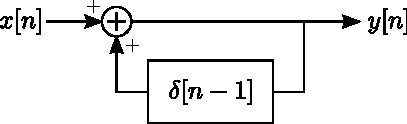
\includegraphics[width=\textwidth]{figuras/difference_equation_accumulator_blocks.pdf}
  \end{minipage}\hfill
  \begin{minipage}[c]{0.55\textwidth}
    \caption{
     Diagrama de bloques de la ecuación en diferencias del acumulador.
    }\label{fig:difference_equation_accumulator_blocks}
  \end{minipage}
\end{figure}

\paragraph{Ejemplo: representación como ecuación en diferencias del sistema de media móvil.} Considérese el sistema de media móvil, dado por la ecuación \ref{eq:seq_and_sys_system_moving_average}, con \(M_1=0\) de forma de que sea causal. En ese caso, la ecuación del sistema es
\begin{equation}\label{eq:seq_and_sys_system_moving_average_causal}
  y[n]=\frac{1}{M_2+1}\sum_{k=0}^{M_2}x[n-k],
\end{equation}
que es una ecuación en diferencias de la forma de la ecuación \ref{eq:seq_and_sys_difference_equation_general}.

Por otro lado, la respuesta al impuso, dada por la ecuación \ref{eq:seq_and_sys_system_moving_average_impulse}, puede escribirse como
\[
 h[n]=\frac{1}{M_2+1}(\delta[n]-\delta[n-M_2-1])*u[n],
\]
que sugiere la representación del sistema media móvil causal puede representarse mediante los sistemas en cascada de la figura \ref{fig:difference_equation_moving_average_blocks}.
\begin{figure}[!htb]
 \begin{center}
 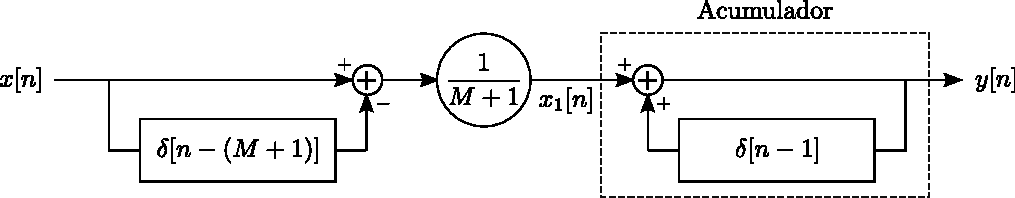
\includegraphics[width=0.88\textwidth]{figuras/difference_equation_moving_average_blocks.pdf}
 \caption{\label{fig:difference_equation_moving_average_blocks} Diagrama de bloques del sistema media móvil.}
 \end{center}
\end{figure}
Para obtener la ecuación en diferencias de este diagrama de bloques, se observa primero que 
\[
 x_1[n]=\frac{1}{M+1}(x[n]-x[n-M_2-1]).
\]
Además, de la ecuación \ref{eq:seq_and_sys_difference_equation_accumulator}, la salida del sistema acumulador cumple la ecuación en diferencias
\[
 y[n]-y[n-1]=x_1[n],
\]
resultando en que 
\begin{align*}\label{eq:seq_and_sys_difference_equation_moving_averge}
 y[n]-y[n-1]=\frac{1}{M+1}(x[n]-x[n-M_2-1]), 
\end{align*}
que es una ecuación en diferencias de la forma \ref{eq:seq_and_sys_difference_equation_general}. En este ejemplo se ve que el sistema media móvil admite mas de una representación en ecuaciones en diferencia, una recursiva y otra no recursiva. Este es un caso muy particular de un sistema recursivo que tiene respuesta al impulso finita.
 
Al igual que en el caso de ecuaciones diferenciales en tiempo continuo, sin restricciones adicionales, una ecuación en diferencias lineal con coeficientes constantes en tiempo discreto no provee una única especificación de la salida dada una entrada. Concretamente, supóngase que para una entrada dada \(x_p[n]\), se determinó de alguna forma que la salida es \(y_p[n]\), tal que se satisface la ecuación \ref{eq:seq_and_sys_difference_equation_general}. Entonces, la misma ecuación con la misma entrada es satisfecha para cualquier salida de la forma 
\[
 y[n]=y_p[n]+y_h[n],
\]
donde \(y_h[n]\) es cualquier solución de la ecuación \ref{eq:seq_and_sys_difference_equation_general} con \(x[n]=0\), es decir, cualquier solución de la ecuación
\begin{equation}\label{eq:seq_and_sys_difference_equation_homogeneous}
 \sum_{k=0}^Na_ky_h[n-k]=0. 
\end{equation}
La ecuación \ref{eq:seq_and_sys_difference_equation_homogeneous} se llama \emph{ecuación en diferencias homogénea} y la solución \(y_h[n]\) se llama \emph{solución homogénea}. La secuencia \(y_h[n]\) es un miembro de la familia de soluciones de la forma
\begin{equation}\label{eq:seq_and_sys_difference_equation_homogeneous_solution}
 y_h[n]=\sum_{m=1}^NA_mz_m^n, 
\end{equation}
donde los coeficientes \(A_m\) pueden elegirse para satisfacer un conjunto de condiciones auxiliares sobre \(y[n]\). Efectivamente, sustituyendo la ecuación \ref{eq:seq_and_sys_difference_equation_homogeneous_solution} en la ecuación \ref{eq:seq_and_sys_difference_equation_homogeneous} se observa que 
\[
 \sum_{k=0}^Na_k\left(\sum_{m=1}^NA_mz_m^{n-k}\right)=0,
\]
y por lo tanto
\[
 \sum_{m=1}^NA_mz_m^n\left(\sum_{k=0}^Na_kz_m^{-k}\right)=0.
\]
Esta ecuación se cumple para cualquier conjunto de valores \(A_m\) cuando los números complejos \(z_m\) con \(m=1,\,2,\,\dots,\,N\) son las raíces del polinomio
\begin{equation}\label{eq:seq_and_sys_difference_equation_homogeneous_solution_Az}
 A(z)=\sum_{k=0}^Na_kz^{-k}. 
\end{equation}

\paragraph{Ejemplo (problema 2.50).} Sea la ecuación en diferencias
\[
 y[n]-\frac{3}{4}y[n-1]+\frac{1}{8}y[n-2]=2x[n-1].
\]
Se determinará la forma general de la solución homogénea. Según la ecuación \ref{eq:seq_and_sys_difference_equation_homogeneous_solution}, en este caso la solución homogénea es de la forma
\[
 y_h[n]=A_1z_1^n+A_2z_2^n,
\]
donde, como indica la ecuación \ref{eq:seq_and_sys_difference_equation_homogeneous_solution_Az}, \(z_1\) y \(z_2\) son las raíces del polinomio 
\[
 A(z)=1-\frac{3}{4}z^{-1}+\frac{1}{8}z^{-2},
\]
que son
\[
 z_{1,\,2}=\dfrac{\dfrac{3}{4}\pm\sqrt{\dfrac{9}{16}-\dfrac{4}{8}}}{2}
  =\dfrac{\dfrac{3}{4}\pm\sqrt{\dfrac{1}{16}}}{2}=\dfrac{\dfrac{3}{4}\pm\dfrac{1}{4}}{2}
\qquad\qquad\Rightarrow\qquad\qquad 
 z_1=\frac{1}{2}
 \qquad\textrm{y}\qquad
 z_2=\frac{1}{4},
\]
resultando en que 
\[
 y_h[n]=A_1\left(\frac{1}{2}\right)^n+A_2\left(\frac{1}{4}\right)^n.
\]
Puede comprobarse que el resultado obtenido es la solución homogénea verificando que cumple la ecuación homogénea para cualquier valor de \(A_1\) y \(A_2\). Efectivamente,
\begin{align*}
 y_h[n]-\frac{3}{4}y_h[n-1]+\frac{1}{8}y_h[n-2]&=A_1\left(\frac{1}{2}\right)^n+A_2\left(\frac{1}{4}\right)^n
  -\frac{3}{4}\left[A_1\left(\frac{1}{2}\right)^{n-1}+A_2\left(\frac{1}{4}\right)^{n-1}\right]\\
  &\qquad+\frac{1}{8}\left[A_1\left(\frac{1}{2}\right)^{n-2}+A_2\left(\frac{1}{4}\right)^{n-2}\right]\\
  &=A_1\left(\frac{1}{2}\right)^n\left(1-\frac{3}{2}+\frac{1}{2}\right)
   +A_2\left(\frac{1}{4}\right)^n\left(1-3+2\right)\\
  &=0.
\end{align*}
Finalmente se determinarán los coeficientes \(A_1\) y \(A_2\) de la solución homogénea si \(y[-1]=1\) y \(y[0]=0\). Con estas condiciones,
\[
 \left\{ 
 \begin{array}{lclclc}
  y[-1] & = & 2A_1+4A_2 & = & 1\\
  y[0] & = & A_1+A_2 & = & 0
 \end{array}
 \right.
 \qquad\qquad\Rightarrow\qquad\qquad
 A_1=-\frac{1}{2}
 \qquad\textrm{y}\qquad
 A_2=\frac{1}{2},
\]
resultando en que 
\[
 y_h[n]=-\frac{1}{2}\left(\frac{1}{2}\right)^n+\frac{1}{2}\left(\frac{1}{4}\right)^n.
\]

La ecuación \ref{eq:seq_and_sys_difference_equation_homogeneous_solution} asume que todas las raíces del polinomio \ref{eq:seq_and_sys_difference_equation_homogeneous_solution_Az} son distintas. Si el polinomio tiene raíces múltiples, la ecuación \ref{eq:seq_and_sys_difference_equation_homogeneous_solution} tiene una forma ligeramente diferente, como se ilustra en el siguiente ejemplo, pero siempre hay \(N\) coeficientes indeterminados.
  
\paragraph{Ejemplo (problema 2.50, continuación).} Sea la ecuación en diferencias
\[
 y[n]-y[n-1]+\frac{1}{4}y[n-2]=2x[n-1].
\]
Se intentará determinar la forma general de la solución homogénea empleando la ecuación \ref{eq:seq_and_sys_difference_equation_homogeneous_solution}. Según esa ecuación, la solución homogénea es de la forma
\[
 y_h[n]=A_1z_1^n+A_2z_2^n,
\]
donde, como indica la ecuación \ref{eq:seq_and_sys_difference_equation_homogeneous_solution_Az}, \(z_1\) y \(z_2\) son las raíces del polinomio 
\[
 A(z)=1-z^{-1}+\frac{1}{4}z^{-2},
\]
que son
\[
 z_{1,\,2}=\dfrac{1\pm\sqrt{1-1}}{2}
  =\frac{1}{2}.
\]
En este caso, el polinomio \(A(z)\) tiene una raíz doble, resultando en que 
\[
 y_h[n]=A_1\left(\frac{1}{2}\right)^n+A_2\left(\frac{1}{2}\right)^n=(A_1+A_2)\left(\frac{1}{2}\right)^n
 =C\left(\frac{1}{2}\right)^n.
\]
Puede mostrarse que el resultado efectivamente satisface la ecuación homogénea para todo valor de \(C\). Sin embargo, como hay solo un coeficiente no pueden imponerse el par de condiciones iniciales, como por ejemplo, \(y[-1]=1\) y \(y[0]=0\). En el caso en que el polinomio \ref{eq:seq_and_sys_difference_equation_homogeneous_solution_Az} tiene una raíz doble, en lugar de la ecuación \ref{eq:seq_and_sys_difference_equation_homogeneous_solution}, la forma general de la solución homogénea es
\[
 y_h[n]=\sum_{m=1}^{N-1}A_mz_m^n+nB_1z_1^n,
\]
donde la raíz duplicada es \(z_1\). De esta ecuación, se obtiene que la solución homogénea general es
\[
 y_h[n]=A_1\left(\frac{1}{2}\right)^n+nB_1\left(\frac{1}{2}\right)^n=(A_1+nB_1)\left(\frac{1}{2}\right)^n.
\]
Puede verificarse que efectivamente es la solución homogénea general, ya que 
\begin{align*}
 y_h[n]-y_h[n-1]+\frac{1}{4}y_h[n-2]&=(A_1+nB_1)\left(\frac{1}{2}\right)^n-[A_1+(n-1)B_1]\left(\frac{1}{2}\right)^{n-1}\\
  &\qquad+\frac{1}{4}[A_1+(n-2)B_1]\left(\frac{1}{2}\right)^{n-2}\\
  &=\left[(A_1+nB_1)-2(A_1+nB_1-B_1)+(A_1+nB_1-2B_1)\right]\left(\frac{1}{2}\right)^n\\
  &=0.
\end{align*}
Si se imponen las condiciones \(y[-1]=1\) y \(y[0]=0\) pueden determinarse los coeficientes \(A_1\) y \(B_1\):
\[
 \left\{ 
 \begin{array}{lclclc}
  y[-1] & = & 2A_1-2B_1 & = & 1\\
  y[0] & = & A_1 & = & 0
 \end{array}
 \right.
 \qquad\qquad\Rightarrow\qquad\qquad
 A_1=0
 \qquad\textrm{y}\qquad
 B_1=-\frac{1}{2},
\]
resultando en que 
\[
 y_h[n]=-\frac{n}{2^{n+1}}.
\]
 
Como \(y_h[n]\) tiene \(N\) coeficientes indeterminados, se necesita un conjunto de \(N\) condiciones auxiliares para la especificación unívoca de \(y[n]\) dado \(x[n]\). Esas condiciones auxiliares pueden consistir en la especificación de los valores de \(y[n]\) para ciertos valores de \(n\), como por ejemplo \(y[-1],\,y[-2],\dots,\,y[-N]\). Los coeficientes se determinan resolviendo el sistema de \(N\) ecuaciones lineales, como se hizo en los ejemplos precedentes.
  
De particular interés son los sistemas lineales e invariantes en el tiempo, y en ese caso, las condiciones auxiliares deben ser consistentes con ese requerimiento. En el capítulo \ref{ch:z_transform}, donde se discute la solución de ecuaciones en diferencias empleando la transformada \(z\), se incorporan implícitamente condiciones de linealidad e invarianza temporal. Como se verá, incluso con las condiciones de linealidad e invarianza temporal, la solución de la ecuación en diferencias no queda unívocamente determinada, y por lo tanto, tampoco el sistema. En particular, en general hay tanto un sistema LTI causal como uno no causal consistente con una ecuación en diferencias dada.

\paragraph{Ejemplo (problema 2.51).} Se considera un sistema con entrada \(x[n]\) y salida \(y[n]\). La relación entre la entrada y la salida está definida por las siguientes dos propiedades:
\begin{enumerate}
 \item \(y[n]-ay[n-1]=x[n]\),
 \item \(y[0]=1\),
\end{enumerate}
y se quiere determinar si el sistema es lineal e invariante en el tiempo.\\
Como \(y[0]=1\) para cualquier entrada, el sistema no es lineal. Por ejemplo, en un sistema lineal, si se duplica la amplitud de la entrada, se duplica la amplitud de la salida, y en este sistema \(y[0]\) tiene un valor fijo.\\
Para estudiar la invarianza temporal, sean las entradas \(x_1[n]=\delta[n]\) y \(x_2[n]=\delta[n-1]\). Como \(x_2[n]=x_1[n-1]\), si el sistema fuera invariante en el tiempo se debería cumplir que \(y_2[n]=y_1[n-1]\). La salida cuando la entrada es \(x_1[n]=\delta[n]\) cuando \(n\leq0\) es
\[
 \begin{array}{lclcl}
  y_1[0]&=&1&&\\
  y_1[1]&=&ay_1[0]+\delta[1]&=&a\\
  y_1[2]&=&ay_1[1]+\delta[2]&=&a^2\\
  &\vdots&&&\\
  y_1[n]&=&a^n,&&
 \end{array}
\]
y la salida cuando la entrada es \(x_2[n]=\delta[n-1]\) cuando \(n\leq0\) es
\[
 \begin{array}{lclcl}
  y_2[0]&=&1&&\\
  y_2[1]&=&ay_2[0]+\delta[0]&=&a+1\\
  y_2[2]&=&ay_2[1]+\delta[1]&=&a^2+a\\
  &\vdots&&&\\
  y_2[n]&=&a^n+a^{n-1}.&&
 \end{array}
\]
Como \(y_2[n]\neq y_1[n-1]\), el sistema no es invariante en el tiempo.\\
Se considera ahora el caso en que la condición inicial es \(y[0]=0\). Para estudiar si el sistema es lineal, se considera primero una entrada arbitraria \(x[n]\). La salida del sistema cuando \(n\geq0\) es 
\begin{align*}
  y[0]&=0\\
  y[1]&=ay[0]+x[1]=x[1]\\
  y[2]&=ay[1]+x[2]=ax[1]+x[2]\\
  y[3]&=ay[2]+x[3]=a^2x[1]+ax[2]+x[3]\\
  &\;\vdots\\
  y[n]&=a^{n-1}x[1]+a^{n-2}x[2]+\cdots+ax[n-1]+x[n],
\end{align*}
es decir,
\[
 y[n]=\sum_{k=0}^{n-1}a^kx[n-k],
 \qquad\qquad\textrm{para }n\geq0.
\]
Para calcular la salida recursivamente para \(n<0\), se escribe la ecuación en diferencias como
\[
 y[n-1]=a^{-1}(y[n]-x[n])
 \qquad\qquad\textrm{con}\qquad\qquad
 y[0]=0.
\]
Luego,
\begin{align*}
  y[-1]&=a^{-1}(y[0]-x[0])=-a^{-1}x[0]\\
  y[-2]&=a^{-1}(y[-1]-x[-1])=-a^{-2}x[0]-a^{-1}x[-1]\\
  y[-3]&=a^{-1}(y[-2]-x[-2])=-a^{-3}x[0]-a^{-2}x[-1]-a^{-1}x[0]\\
  &\;\vdots\\
  y[n]&=-a^{n}x[0]-a^{n+1}x[-1]-\cdots-a^{-2}x[n+2]-a^{-1}x[n+1],
\end{align*}
es decir,
\[
 y[n]=-\sum_{k=-1}^{n}a^kx[n-k],
 \qquad\qquad\textrm{para }n<0.
\] 
Se obtuvo que dada una entrada \(x[n]\), la salida es
\begin{equation}\label{eq:seq_and_sys_exercise_2_51_output}
 y[n]=
 \left\{ 
 \begin{array}{ll}
  \displaystyle\sum_{k=0}^{n-1}a^kx[n-k],&n\geq0\\
  \displaystyle-\sum_{k=-1}^{n}a^kx[n-k],&n<0.
 \end{array}
 \right. 
\end{equation}
Sean \(y_1[n]\) y \(y_2[n]\) las correspondientes salidas cuando las entradas son \(x_1[n]\) y  \(x_2[n]\), y se considera la entrada
\[
 x_3[n]=\alpha x_1[n]+\beta x_2[n].
\]
De la ecuación \ref{eq:seq_and_sys_exercise_2_51_output}, la salida cuando \(n\geq0\) es
\begin{align*}
 y_3[n]&=\sum_{k=0}^{n-1}a^kx_3[n-k]\\
  &=\sum_{k=0}^{n-1}a^k(\alpha x_1[n-k]+\beta x_2[n-k])\\
  &=\alpha\sum_{k=0}^{n-1}a^kx_1[n-k]+\beta\sum_{k=0}^{n-1}a^kx_2[n-k]\\
  &=\alpha y_1[n]+\beta y_2[n].
\end{align*}
De forma análoga, cuando \(n<0\), la salida es
\begin{align*}
 y_3[n]&=-\sum_{k=-1}^{n}a^kx_3[n-k]\\
  &=-\sum_{k=-1}^{n}a^k(\alpha x_1[n-k]+\beta x_2[n-k])\\
  &=\alpha\left(-\sum_{k=-1}^{n}a^kx_1[n-k]\right)+\beta\left(-\sum_{k=-1}^{n}a^kx_2[n-k]\right)\\
  &=\alpha y_1[n]+\beta y_2[n].
\end{align*}
Se concluye que el sistema es lineal.
 
Si un sistema es caracterizado por una ecuación en diferencias lineal con coeficientes constantes y además es restringido a ser lineal, invariante en el tiempo y causal, entonces la solución es única. En este caso, se dice que las condiciones auxiliares son \emph{condiciones iniciales de reposo}. Concretamente, la información auxiliar es que si la entrada \(x[n]\) es nula para \(n\) menor a algún instante \(n_0\), la salida \(y[n]\) se restringe a ser nula para \(n\) menor que \(n_0\). Esto provee condiciones iniciales suficientes para obtener \(y[n]\) unívocamente para \(n\geq n_0\) recursivamente.
 
\paragraph{Ejemplo.} Se considera nuevamente el sistema definido por la ecuación en diferencias
\[
 y[n]-ay[n-1]=x[n]
\]
del ejemplo anterior, y se impone la condición adicional de que si la entrada es nula para \(n\leq n_0\), la salida es nula en \(n\leq n_0\). Se mostrará que con esta imposición, el sistema en invariante en el tiempo. Sea la entrada
\[
 x_1[n]=x[n]u[n],
\]
donde \(x[n]\) es una secuencia arbitraria. Definida de esta forma se cumple que \(x_1[n]=0\) en \(n<0\), y se impone que la salida \(y_1[n]=0\) en \(n<0\). Esto equivale a imponer la condición auxiliar \(y_1[-1]=0\). En ese caso, la salida para \(n\geq0\) es
\begin{align*}
  y_1[0]&=ay_1[-1]+x_1[0]=x[0]\\
  y_1[1]&=ay_1[0]+x_1[1]=ax[0]+x[1]\\
  y_1[2]&=ay_1[1]+x_1[2]=a^2x[0]+ax[1]+x[2]\\
  &\;\vdots\\
  y_1[n]&=a^{n}x[0]+a^{n-1}x[1]+\cdots+ax[n-1]+x[n],
\end{align*}
es decir,
\begin{equation}\label{eq:seq_and_sys_exercise_2_51_ext_output}
 y_1[n]=\sum_{k=0}^{n}a^kx[n-k],
 \qquad\qquad\textrm{para }n\geq0. 
\end{equation}
Para calcular la salida recursivamente para \(n<0\), se escribe la ecuación en diferencias como
\[
 y[n-1]=a^{-1}(y[n]-x[n])
 \qquad\qquad\textrm{con}\qquad\qquad
 y[-1]=0.
\]
Luego,
\begin{align*}
  y_1[-2]&=a^{-1}(y_1[-1]-x_1[-1])=0\\
  y_1[-3]&=a^{-1}(y_1[-2]-x_1[-2])=0\\
  &\;\vdots\\
  y_1[n]&=0,
  \qquad\qquad\textrm{para }n<0.
\end{align*}
Puede verse imponiendo como entrada \(x[n]=\delta[n]\), que la respuesta al impulso del sistema es
\[
 h[n]=a^nu[n],
\]
y por lo tanto, el sistema es causal. Además, la ecuación \ref{eq:seq_and_sys_exercise_2_51_ext_output} se puede escribir como
\[
 y_1[n]=\sum_{k=0}^{n}a^kx[n-k]=\sum_{k=-\infty}^\infty h[k]x_1[n-k]=h[n]*x_1[n].
\]
Se considera ahora la entrada \(x_2[n]=x_1[n-n_0]=x[n-n_0]u[n-n_0]\), donde \(n_0\) es un entero arbitrario. Ahora, \(x_2[n]=0\) en \(n<n_0\), y la restricción de que \(y_2[n]=0\) en \(n<n_0\) corresponde a la condición inicial \(y_2[n_0-1]=0\) de la ecuación en diferencias. Con esta condición inicial, la salida para \(n\geq n_0\) es
\begin{align*}
  y_2[n_0]&=ay_2[n_0-1]+x_2[n_0]=x[0]\\
  y_2[n_0+1]&=ay_2[n_0]+x_2[n_0+1]=ax[0]+x[1]\\
  &\;\vdots\\
  y_2[n_0+m]&=a^{m}x[0]+a^{m-1}x[1]+\cdots+ax[m-1]+x[m],
\end{align*}
es decir,
\[
 y_2[n_0+m]=\sum_{k=0}^{m}a^kx[m-k],
 \qquad\qquad\textrm{para }m\geq0. 
\]
Esto también se puede escribir como
\[
 y_2[n]=\sum_{k=0}^{n-n_0}a^kx[n-n_0-k],
 \qquad\qquad\textrm{para }n\geq n_0.
\]
resolviendo la recursión puede verificarse además que \(y_2[n]=0\) si \(n<n_0\). Por lo tanto, reemplazando \(n\) por \(n-n_0\) en la ecuación \ref{eq:seq_and_sys_exercise_2_51_ext_output}, se deduce que 
\[
 y_2[n]=y_1[n-n_0]
\]
para todo \(n_0\). Considerando que \(x_2[n]=x_1[n-n_0]\), se concluye que el sistema es invariante en el tiempo.
 
\section{Representación de señales y sistemas en el dominio de la frecuencia}\label{sec:seq_and_sys_frequency_domain_representation} 
 
Las secuencias sinusoidales y exponenciales complejas juegan un rol particularmente importante en la representación de señales en tiempo discreto. Esto se debe a que las secuencias exponenciales complejas son funciones propias de los sistemas LTI, y la respuesta de un sistema LTI a una entrada sinusoidal es una secuencia sinusoidal con la misma frecuencia de la entrada pero con amplitud y fase determinadas por el sistema.
 
\subsection{Funciones propias de los sistemas LTI} 

La propiedad de función propia de la exponenciales complejas para los sistemas LTI se obtiene directamente de la definición \ref{eq:seq_and_sys_convolution_definition} de la suma de convolución. Específicamente, si la entrada a un sistema LTI con respuesta al impulso \(h[n]\) es \(x[n]=e^{j\omega n}\) para \(-\infty<n<\infty\), de la ecuación \ref{eq:seq_and_sys_convolution_definition}, la salida es
\begin{align*}
 y[n]&=\sum_{k=-\infty}^{\infty}h[k]e^{j\omega(n-k)}\\
   &=e^{j\omega n}\sum_{k=-\infty}^{\infty}h[k]e^{-j\omega k}.
\end{align*}
Definiendo a la constante compleja
\begin{equation}\label{eq:seq_and_sys_frequency_response_definition}
 H(e^{j\omega})=\sum_{k=-\infty}^{\infty}h[k]e^{-j\omega k}, 
\end{equation}
la salida es
\begin{equation}\label{eq:seq_and_sys_frequency_response_output}
 y[n]=H(e^{j\omega})e^{j\omega n}. 
\end{equation}
En consecuencia, \(e^{j\omega n}\) es una función propia del sistema, y valor propio asociado es \(H(e^{j\omega})\). El valor propio \(H(e^{j\omega})\) se llama \emph{respuesta en frecuencia} del sistema y describe el cambio de la magnitud y la fase de la exponencial compleja de entrada en función de la frecuencia.

En la sección \ref{sec:fourier_transform_representation} se verá que un amplio conjunto de señales se puede representar como la combinación lineal de exponenciales complejas como
\begin{equation}\label{eq:seq_and_sys_complex_exponential_linear_combination}
 x[n]=\sum_k\alpha_k e^{j\omega_kn}. 
\end{equation}
Del principio de superposición, dado por la ecuación \ref{eq:seq_and_sys_sys_properties_superposition}, y la ecuación \ref{eq:seq_and_sys_frequency_response_output}, la correspondiente salida de un sistema LTI es
\[
 y[n]=\sum_k\alpha_kH(e^{j\omega_k})e^{j\omega_kn}.
\]
Por lo tanto, si se puede encontrar una representación de la entrada como superposición de secuencias exponenciales complejas, es posible obtener la salida si se conoce la respuesta en frecuencia del sistema para todas las frecuencias \(\omega\).

\paragraph{Ejemplo: respuesta sinusoidal de los sistemas LTI.} Sea la entrada sinusoidal
\[
 x[n]=A\cos(\omega_0n+\phi)=\underbrace{\frac{A}{2}e^{j\phi}e^{j\omega_0n}}_{\displaystyle x_1[n]}+\underbrace{\frac{A}{2}e^{-j\phi}e^{-j\omega_0n}}_{\displaystyle x_2[n]}.
\]
De la ecuación \ref{eq:seq_and_sys_frequency_response_output}, la respuesta a \(x_1[n]\) es
\[
 y_1[n]=H(e^{j\omega_0})\frac{A}{2}e^{j\phi}e^{j\omega_0n}
\]
y la respuesta a \(x_2[n]\) es
\[
 y_2[n]=H(e^{-j\omega_0})\frac{A}{2}e^{-j\phi}e^{-j\omega_0n}.
\]
Por lo tanto, por el principio de superposición, la respuesta total es
\begin{align*}
 y[n]&=\frac{A}{2}\left[H(e^{j\omega_0})e^{j\phi}e^{j\omega_0n}+H(e^{-j\omega_0})e^{-j\phi}e^{-j\omega_0n}\right]\\
  &\overset{(a)}{=}\frac{A}{2}\left[H(e^{j\omega_0})e^{j\phi}e^{j\omega_0n}+H^*(e^{j\omega_0})e^{-j\phi}e^{-j\omega_0n}\right]\\
  &=A\Re\left[H(e^{j\omega_0})e^{j\phi}e^{j\omega_0n}\right],
\end{align*}
donde en \((a)\) se consideró que si la respuesta al impulso \(h[n]\) del sistema es real, se cumple que \(H(e^{-j\omega_0})=H^*(e^{j\omega_0})\). Expresando la respuesta en frecuencia en \(\omega_0\) como
\[
 H(e^{j\omega_0})=G_0e^{j\theta_0},
 \qquad\qquad\textrm{donde}\qquad\qquad 
 G_0=|H(e^{j\omega_0})|
 \qquad\qquad\textrm{y}\qquad\qquad
 \theta_0=\angle H(e^{j\omega_0}),
\]
resulta en que 
\begin{equation}\label{eq:seq_and_sys_frequency_response_output_sinusoidal}
 y[n]=AG_0\cos(\omega_0n+\phi+\theta_0). 
\end{equation}
\begin{figure}[!htb]
 \begin{center}
 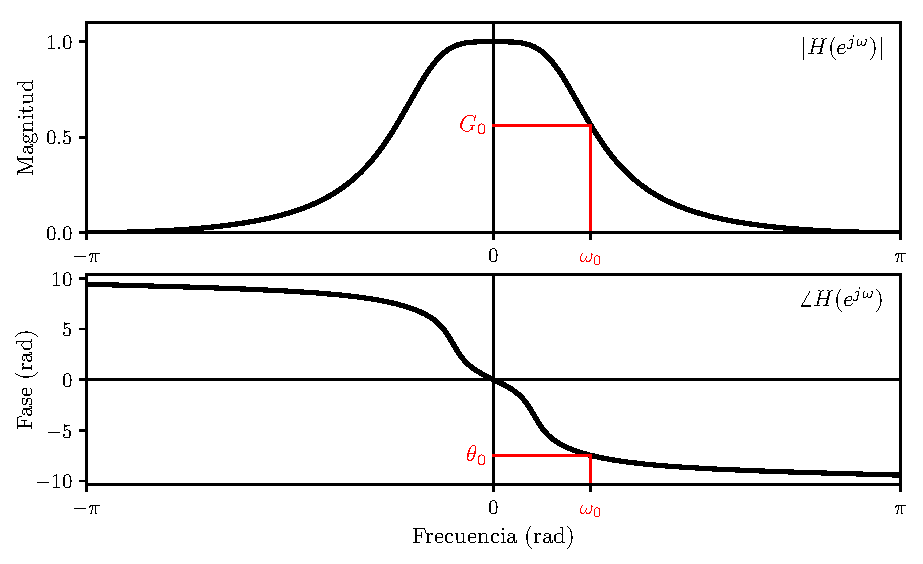
\includegraphics[width=0.90\textwidth]{figuras/seq_and_sys_frequency_response.pdf}
 \caption{\label{fig:seq_and_sys_frequency_response} Respuesta en magnitud \(|H(e^{j\omega})|\) y fase \(\angle H(e^{j\omega})\) de un sistema LTI. Se trata de un filtro pasabajos.}
 \end{center}
\end{figure}
Si la entrada a un sistema LTI es una secuencia sinusoidal de frecuencia \(\omega_0\) y la respuesta en magnitud y fase del sistema en esa frecuencia es respectivamente \(G_0\) y \(\theta_0\), como se muestra en la figura \ref{fig:seq_and_sys_frequency_response}, la ecuación \ref{eq:seq_and_sys_frequency_response_output_sinusoidal} indica que la salida es una secuencia sinusoidal con la misma frecuencia \(\omega_0\) pero con amplitud alterada un factor \(G_0\) y fase desplazada una cantidad \(\theta_0\) radianes. Este sistema se llama \emph{filtro pasabajos}, ya que deja pasar las bajas frecuencias inalteradas e impide pasar las frecuencias altas.

\begin{figure}[!htb]
 \begin{center}
 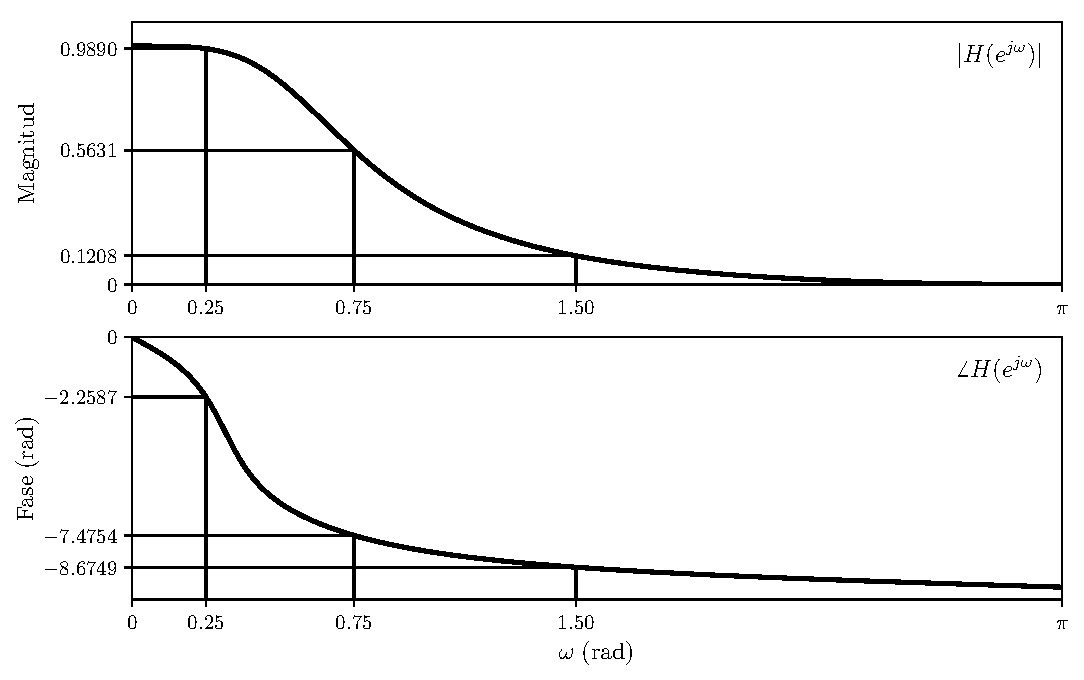
\includegraphics[width=\textwidth]{figuras/seq_and_sys_frequency_response_output_response.pdf}
 \caption{\label{fig:seq_and_sys_frequency_response_output_response} Sistema pasabajos LTI. Se especifica la respuesta en magnitud y en fase en las frecuencias \(0.25\), \(0.75\) y \(1.5\) radianes. Observar que la respuesta en fase está \emph{desdoblada} (\emph{unwrapped}).}
 \end{center}
\end{figure}
A continuación se ilustra el resultado de la ecuación \ref{eq:seq_and_sys_frequency_response_output_sinusoidal} con un ejemplo numérico. Sea el filtro pasabajos LTI cuya respuesta en frecuencia se muestra en la figura \ref{fig:seq_and_sys_frequency_response_output_response}, y se consideran las entradas
\[
 x_i[n]=\sen\omega_in,
 \qquad\qquad\textrm{para}\qquad\qquad i=0,\,1,\,2,
\]
donde \(\omega_0=0.25\), \(\omega_1=0.75\) y \(\omega_2=1.5\) radianes.
Según la ecuación \ref{eq:seq_and_sys_frequency_response_output_sinusoidal}, las correspondientes salidas son
\begin{equation}\label{eq:seq_and_sys_frequency_response_output_sinusoidal_zero_phase}
 y_i[n]=G_i\sen(\omega_in+\theta_i), 
\end{equation}
donde \(G_i\) y \(\theta_i\) son respectivamente la respuesta en magnitud y en fase del sistema en la frecuencia \(\omega_i\), es decir,
\[
 G_i=|H(e^{j\omega_i})|
 \qquad\qquad\textrm{y}\qquad\qquad
 \theta_i=\angle H(e^{j\omega_i}).
\]
En la figura \ref{fig:seq_and_sys_frequency_response_output_response_gain} se muestran las entradas \(x_i[n]\) y las correspondientes salidas \(y_i[n]\). Se observa que, acorde a la ecuación \ref{eq:seq_and_sys_frequency_response_output_sinusoidal_zero_phase}, la salida tiene la misma frecuencia que la entrada, pero con amplitud modificada según la repuesta en magnitud del sistema en la frecuencia \(\omega_i\). 
\begin{figure}[!htb]
 \begin{center}
 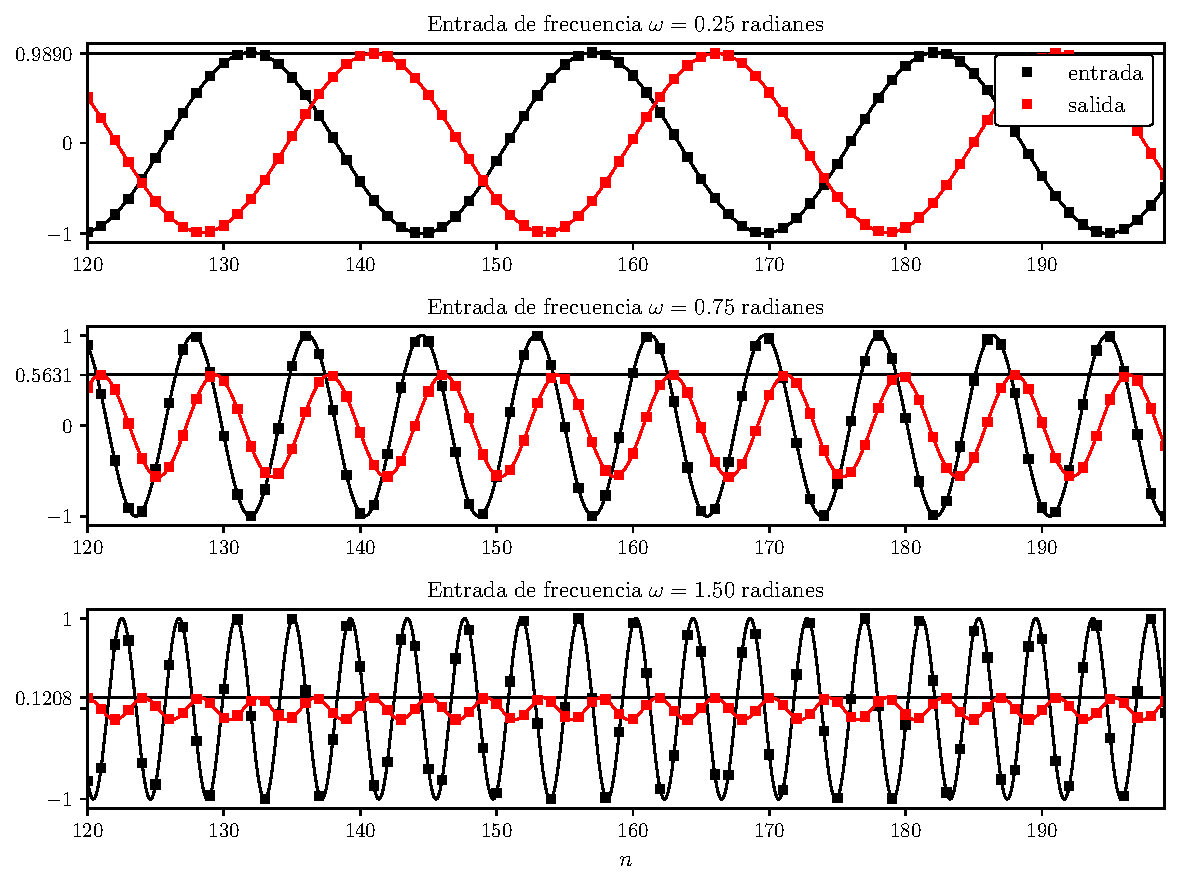
\includegraphics[width=\textwidth]{figuras/seq_and_sys_frequency_response_output_response_gain.pdf}
 \caption{\label{fig:seq_and_sys_frequency_response_output_response_gain} Ilustración de la respuesta en magnitud de un sistema LTI para una señal sinusoidal. La amplitud de la salida es acorde a la repuesta en magnitud del sistema. La línea continua que interpola las muestras es solo para mejor visualización.}
 \end{center}
\end{figure}

Respecto a la fase de la sinusoide de salida, la ecuación \ref{eq:seq_and_sys_frequency_response_output_sinusoidal} indica que a la fase de la entrada se le adiciona la respuesta en fase del sistema en la frecuencia de la sinusoide. La alteración de la fase puede interpretarse como un retardo de la señal. Efectivamente, considerando que la ecuación \ref{eq:seq_and_sys_frequency_response_output_sinusoidal_zero_phase} puede escribirse como 
\[
 y_i[n]=G_i\sen\left\{\omega_i\left[n-\left(-\dfrac{\theta_i}{\omega_i}\right)\right]\right\}, 
\]
la sinusoide de salida está retardada una cantidad de \(-\theta_i/\omega_i\) muestras respecto a la sinusoide de entrada. Esto motiva a la definición del \emph{retardo de fase} de un sistema como
\begin{equation}\label{eq:seq_and_sys_phase_delay_definition}
 \tau_\phi(\omega)=-\frac{\angle H(e^{j\omega})}{\omega}.
\end{equation}
\begin{figure}[!htb]
 \begin{center}
 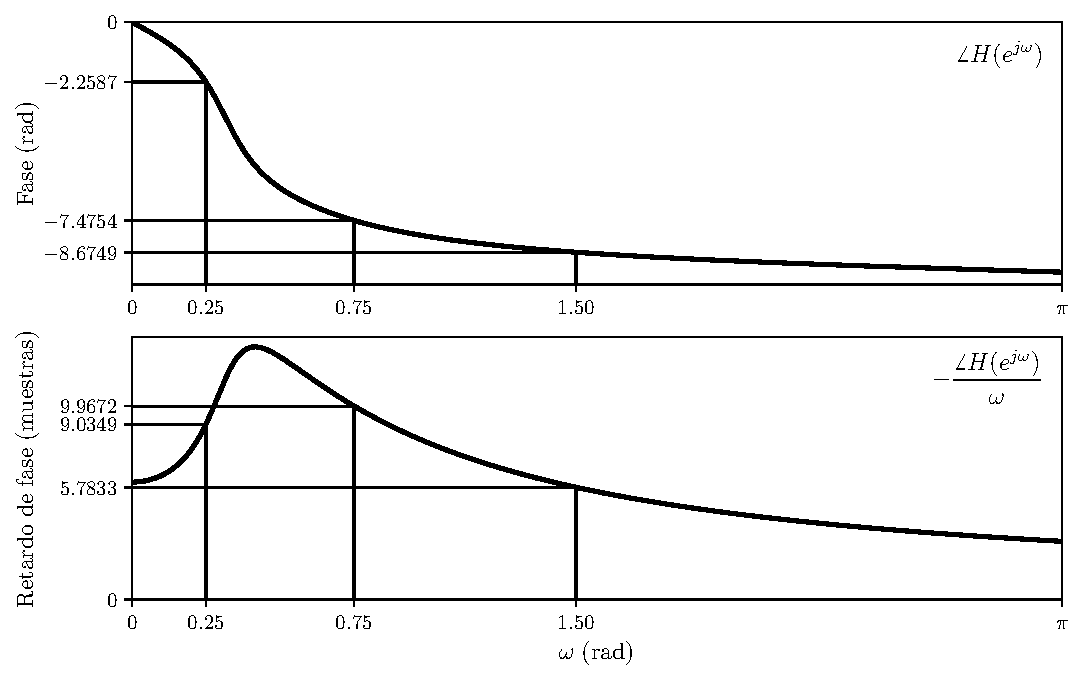
\includegraphics[width=\textwidth]{figuras/seq_and_sys_frequency_response_output_phase_response.pdf}
 \caption{\label{fig:seq_and_sys_frequency_response_output_phase_response} Respuesta en fase y retardo de fase del sistema. El retardo de fase se interpreta como la cantidad de muestras que el sistema retarda a una sinusoide de entrada.}
 \end{center}
\end{figure}
En la figura \ref{fig:seq_and_sys_frequency_response_output_phase_response} se muestra la respuesta en fase y el retardo de fase para el sistema del ejemplo, y se especifica la fase y el retardo de fase en las frecuencias de las sinusoides de entrada.
\begin{figure}[!htb]
 \begin{center}
 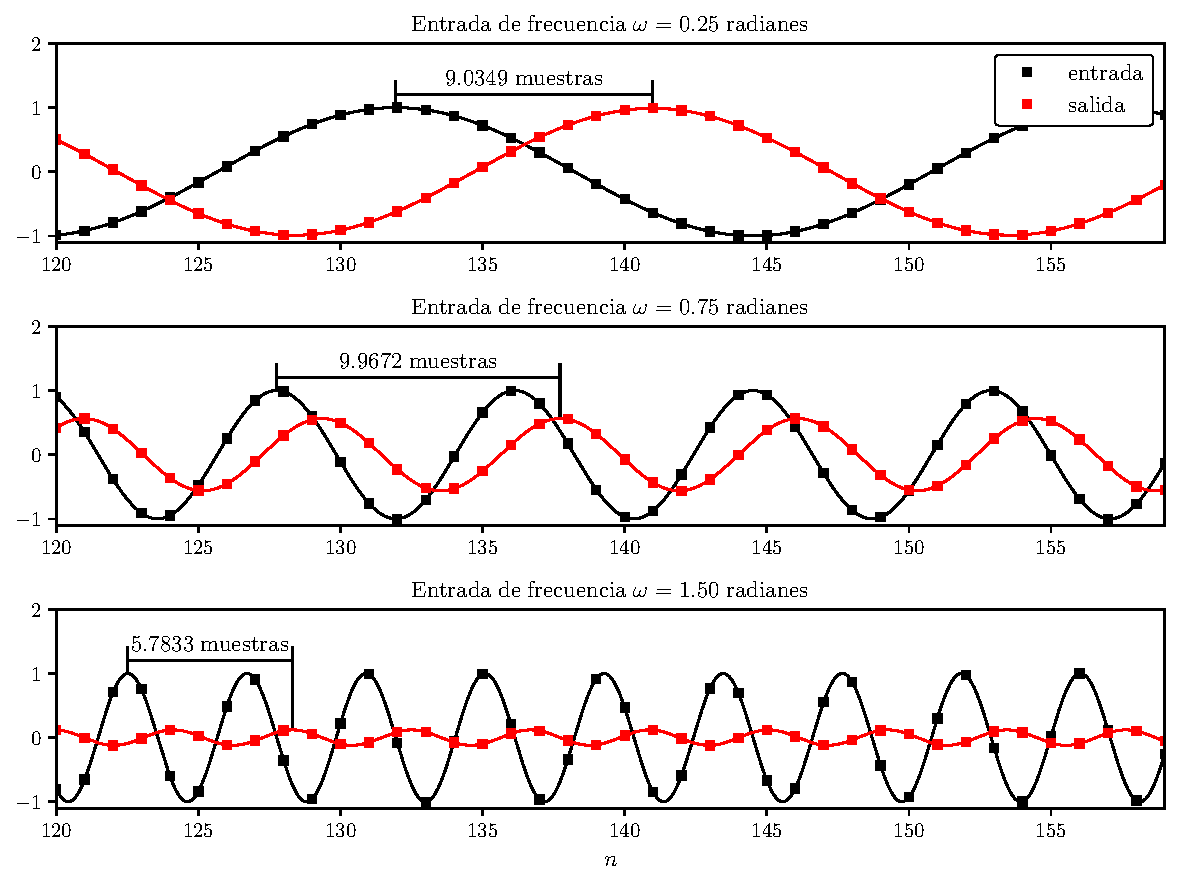
\includegraphics[width=\textwidth]{figuras/seq_and_sys_frequency_response_output_response_phase.pdf}
 \caption{\label{fig:seq_and_sys_frequency_response_output_response_phase} Ilustración del retardo de fase de un sistema. Se interpreta como el retardo en muestras de la señal sinusoidal de tiempo continuo subyacente a la señal sinusoidal de tiempo discreto. Por supuesto que los instantes de muestreo no cambian.}
 \end{center}
\end{figure}
En la figura \ref{fig:seq_and_sys_frequency_response_output_response_phase} se muestran las entradas y las salidas y se ilustra la interpretación del retardo de fase. Observar que el retardo de fase, que no necesariamente es un número entero, es el retardo temporal de la sinusoide de tiempo continuo subyacente a la sinusoide en tiempo discreto. En el caso de las señales de entrada de este ejemplo, las señales en tiempo continuo subyacentes son
\[
 x_i(t)=\sen\omega_it,
\]
donde las unidades de \(t\) son segundos y en los instantes de muestreo \(t=n\) segundos, y el valor \(\omega_i\) es el mismo que el de la señal en tiempo discreto pero las unidades son radianes/segundo en lugar de radianes o radianes/muestra. En la figura \ref{fig:seq_and_sys_frequency_response_output_response_phase} la señal continua subyacente en cada caso está representada con trazo continuo. La señal equivalente en tiempo continuo de las salidas es
\[
 y_i(t)=G_i\sen\left\{\omega_i\left[t-\tau_\phi(\omega_i)\right]\right\},
\]
donde el retardo de fase \(\tau_\phi(\omega_i)\) tiene el mismo valor que en el caso discreto pero las unidades son segundos en lugar de adimensionado o muestras. En la sección 4.5 de \cite{oppenheim2009discrete} se da una interpretación de un retardo no entero. 

\paragraph{Ejemplo: respuesta en frecuencia del sistema de media móvil} La respuesta al impulso del sistema de media móvil está dado por la ecuación \ref{eq:seq_and_sys_system_moving_average} es (ver la ecuación \ref{eq:seq_and_sys_system_moving_average_impulse})
\[
 h[n]=
 \left\{ 
 \begin{array}{ll}
  \dfrac{1}{M_1+M_2+1}, & -M_1\leq n\leq M_2,\\
  0, & \textrm{en otro caso.}
 \end{array}
 \right.
\]
Por lo tanto, la respuesta en frecuencia es
\[
 H(e^{j\omega})=\frac{1}{M_1+M_2+1}\sum_{n=-M_1}^{M_2}e^{-j\omega n}.
\]
Para el sistema causal, \(M_1=0\) y la respuesta en frecuencia queda
\[
 H(e^{j\omega})=\frac{1}{M_2+1}\sum_{n=0}^{M_2}e^{-j\omega n},
\]
y empleando el resultado de la suma de los primeros \(M_2+1\) términos de una serie geométrica, se puede escribir como
\begin{align*}
 H(e^{j\omega})&=\frac{1}{M_2+1}\left(\frac{1-e^{-j\omega M_2+1}}{1-e^{-j\omega}}\right)\\
  &=\frac{1}{M_2+1}\frac{\left[e^{j\omega(M_2+1)/2}-e^{-j\omega(M_2+1)/2}\right]e^{-j\omega(M_2+1)/2}}{\left(e^{j\omega/2}-e^{-j\omega/2}\right)e^{j\omega/2}}\\
\end{align*}
resultando en
\begin{equation}\label{eq:seq_and_sys_system_moving_average_causal_freq_response}
 H(e^{j\omega})=\frac{1}{M_2+1}\,\frac{\sen\left[\omega(M_2+1)/2\right]}{\sen\omega/2}e^{-j\omega M_2/2}. 
\end{equation}
La magnitud y la fase de \(H(e^{j\omega})\) para este caso con \(M_2=4\) se muestra en la figura \ref{fig:example_02_16_moving_average_freq_response}.
\begin{figure}[!htb]
 \begin{center}
 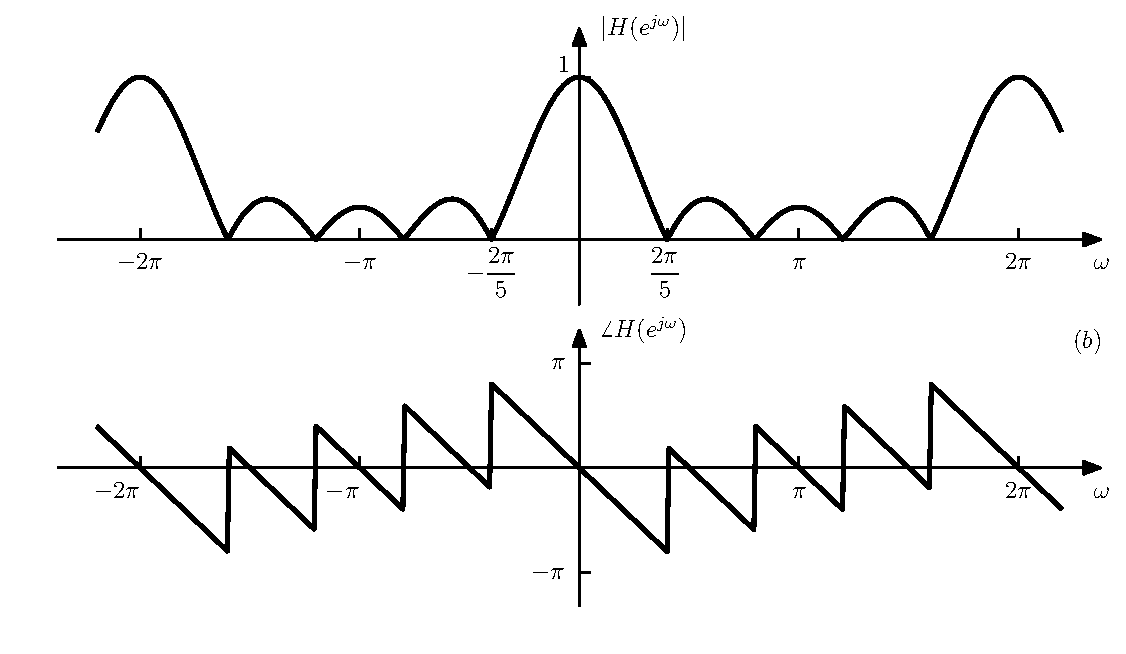
\includegraphics[width=0.98\textwidth]{figuras/example_02_16_moving_average_freq_response.pdf}
 \caption{\label{fig:example_02_16_moving_average_freq_response} Magnitud y fase de la respuesta en frecuencia del sistema de media móvil causal con \(M_2=4\).}
 \end{center}
\end{figure}

\section{Representación de secuencias mediante transformadas de Fourier}\label{sec:fourier_transform_representation}

Una ventaja de la representación en frecuencias de los sistemas LTI es que a menudo la interpretación del comportamiento del sistema se observa inmediatamente en el dominio de las frecuencias, como es el caso de los filtros selectores de frecuencias. En esta sección se estudia como encontrar representaciones de señales de la forma de la ecuación \ref{eq:seq_and_sys_complex_exponential_linear_combination}.

Muchas secuencias pueden representarse mediante una integral de Fourier como
\begin{equation}\label{eq:seq_and_sys_dtft_inverse_definition}
 x[n]=\frac{1}{2\pi}\int_{-\pi}^\pi X(e^{j\omega})e^{j\omega n}\,d\omega,
\end{equation}
donde 
\begin{equation}\label{eq:seq_and_sys_dtft_definition}
 X(e^{j\omega})=\sum_{n=-\infty}^\infty x[n]e^{-j\omega n}.
\end{equation}
Las ecuaciones \ref{eq:seq_and_sys_dtft_inverse_definition} y \ref{eq:seq_and_sys_dtft_definition} son la representación de Fourier de la secuencia. La ecuación \ref{eq:seq_and_sys_dtft_inverse_definition}, la \emph{transformada de Fourier inversa}, es una ecuación de síntesis. Representa a \(x[n]\) como una superposición de sinusoidales complejas infinitesimalmente pequeñas de la forma
\[
 \frac{1}{2\pi}X(e^{j\omega})e^{j\omega n}\,d\omega,
\]
con \(\omega\) variando en un intervalo de largo \(2\pi\) y donde \(X(e^{j\omega})\) determina el peso relativo de cada componente sinusoidal complejo. La ecuación \ref{eq:seq_and_sys_dtft_definition}, la \emph{transformada de Fourier}, es una expresión para calcular \(X(e^{j\omega})\), es decir, para analizar la secuencia \(x[n]\) para determinar cuanto de cada componente de frecuencia se necesita para sintetizar \(x[n]\) mediante la ecuación \ref{eq:seq_and_sys_dtft_inverse_definition}. La ecuación \ref{eq:seq_and_sys_dtft_definition} es referida explícitamente como la \emph{transformada de Fourier en tiempo discreto} (\emph{DTFT}, Discrete-Time Fourier Transform).

En general la transformada de Fourier es una función compleja de \(\omega\), y se puede representar en forma rectangular como
\[
 X(e^{j\omega})=X_R(e^{j\omega})+jX_I(e^{j\omega})
\]
o en forma polar como
\[
 X(e^{j\omega})=|X(e^{j\omega})|e^{j\angle X(e^{j\omega})},
\]
donde \(|X(e^{j\omega})|\) representa la magnitud y \(\angle X(e^{j\omega})\) la fase. Observar que la fase \(\angle X(e^{j\omega})\) no está unívocamente especificada, ya que puede sumarse cualquier múltiplo de \(2\pi\) a cualquier valor de frecuencia \(\omega\) sin alterar el resultado de la exponencial compleja. Cuando se hace referencia al valor principal, es decir, cuando \(\angle X(e^{j\omega})\) se restringe al rango de valores entre \(-\pi\) y \(\pi\), se denota como \(\ARG[X(e^{j\omega})]\). Cuando se hace referencia a una función de fase que es continua en \(\omega\) para \(0<\omega<\pi\) se emplea la notación \(\arg[X(e^{j\omega})]\).
 
Comparando las ecuaciones \ref{eq:seq_and_sys_frequency_response_definition} y \ref{eq:seq_and_sys_dtft_definition}, es claro que la respuesta en frecuencia de un sistema LTI es la transformada de Fourier de la respuesta al impulso. La respuesta al impulso puede obtenerse a partir de la respuesta en frecuencia mediante la transformada de Fourier inversa como
\[
 h[n]=\frac{1}{2\pi}\int_{-\pi}^\pi H(e^{j\omega})e^{j\omega n}\,d\omega.
\]

La transformada de Fourier es una función periódica de período \(2\pi\). Para representar funciones periódicas puede emplearse la serie de Fourier, y efectivamente la ecuación \ref{eq:seq_and_sys_dtft_definition} es de la forma de la representación en series de Fourier de la función periódica \(X(e^{j\omega})\), y la ecuación \ref{eq:seq_and_sys_dtft_inverse_definition} es de la forma de la integral empleada para obtener los coeficientes de la serie de Fourier.

La clase de señales que pueden representarse mediante la ecuación \ref{eq:seq_and_sys_dtft_inverse_definition} son aquellas para las que la suma infinita de la ecuación \ref{eq:seq_and_sys_dtft_definition} converge. Una condición suficiente para la convergencia de dicha suma es que la secuencia \(x[n]\) sea absolutamente sumable. En ese caso, puede mostrarse que la serie converge uniformemente a una función continua de \(\omega\). Como una secuencia estable es absolutamente sumable, todas las secuencias estables tienen transformada de Fourier. Equivalentemente, todo sistema estable tiene respuesta en frecuencia finita y continua. Las secuencias de largo finito y los sistemas FIR también tienen transformada de Fourier.
 
Algunas secuencias no son absolutamente sumables pero son cuadráticamente sumables, es decir, tienen energía finita
\[
 E_x=\sum_{n=-\infty}^\infty |x[n]|^2<\infty,
\]
que es una condición mas débil que la de sumabilidad absoluta. Estas secuencias pueden representarse mediante una transformada de Fourier pero relajando la condición de convergencia uniforme de la suma que define a \(X(e^{j\omega})\). En este caso, la convergencia es en media cuadrática, es decir,
\[
 \lim_{M\to\infty}\int_{-\pi}^\pi|X(e^{j\omega})-X_M(e^{j\omega})|^2\,d\omega=0,
\]
donde 
\[
 X_M(e^{j\omega})=\sum_{n=-M}^Mx[n]e^{-j\omega n}.
\]
El error \(|X(e^{j\omega})-X_M(e^{j\omega})|\) puede no tender a cero para cada valor de \(\omega\) cuando \(M\to\infty\) pero si lo hace la energía total del error. Un ejemplo de este caso es el pasabajos ideal.
 
\paragraph{Ejemplo: transformada de Fourier de secuencias exponenciales complejas} Se considera la secuencia \(x[n]\) cuya transformada de Fourier es el tren de impulsos periódico
\begin{equation}\label{eq:seq_and_sys_complex_exponential_dtft}
 X(e^{j\omega})=\sum_{r=-\infty}^\infty2\pi\delta(\omega-\omega_0+2\pi r), 
\end{equation}
donde \(-\pi<\omega_0<\pi\). Para determinar \(x[n]\) puede aplicarse la ecuación \ref{eq:seq_and_sys_dtft_inverse_definition} de transformada inversa de Fourier a \(X(e^{j\omega})\). Como el intervalo de integración en la ecuación \ref{eq:seq_and_sys_dtft_inverse_definition} se extiende sobre \(-\pi<\omega<\pi\) solo el impulso con \(r=0\) pertenece a dicho intervalo, y por lo tanto,
\[
 x[n]=\frac{1}{2\pi}\int_{-\pi}^\pi2\pi\delta(\omega-\omega_0)e^{j\omega n}\,d\omega=e^{j\omega_0n}.
\]
Se obtuvo que 
\begin{equation}\label{eq:seq_and_sys_complex_exponential_dtft_pair}
 x[n]=e^{j\omega_0n}\;\overset{\mathcal{F}}{\longleftrightarrow}\;X(e^{j\omega})=\sum_{r=-\infty}^\infty2\pi\delta(\omega-\omega_0+2\pi r). 
\end{equation}
En este caso, \(x[n]\) no es absolutamente ni cuadráticamente sumable, y \(|X(e^{j\omega})|\) no es finita para todo \(\omega\). La igualdad matemática  
\[
 \sum_{n=-\infty}e^{j\omega n}e^{-j\omega_0}=\sum_{r=-\infty}^\infty2\pi\delta(\omega-\omega_0+2\pi r),
\]
que proviene de sustituir \(x[n]=e^{j\omega_0n}\) en la ecuación \ref{eq:seq_and_sys_dtft_definition} e igualar el resultado con la ecuación \ref{eq:seq_and_sys_complex_exponential_dtft}, debe interpretarse en el sentido de las funciones generalizadas. Con \(\omega_0=0\) se obtiene el par de transformadas
\begin{equation}\label{eq:seq_and_sys_constant_dtft_pair}
 x[n]=1\overset{\mathcal{F}}{\longleftrightarrow}X(e^{j\omega})=\sum_{r=-\infty}^\infty2\pi\delta(\omega+2\pi r). 
\end{equation} 
Además, considerando que 
\[
 \cos\omega_0n=\frac{1}{2}e^{j\omega_0n}+\frac{1}{2}e^{-j\omega_0n}
  \qquad\qquad\textrm{y}\qquad\qquad
 \sin\omega_0n=\frac{1}{2j}e^{j\omega_0n}-\frac{1}{2j}e^{-j\omega_0n},
\]
y empleando la propiedad de linealidad de la transformada de Fourier, de \ref{eq:seq_and_sys_complex_exponential_dtft_pair} se deduce inmediatamente que
\begin{equation}\label{eq:seq_and_sys_sin_cos_dtft_pair}
\begin{array}{ccc}
 \cos\omega_0n&\overset{\mathcal{F}}{\longleftrightarrow}&\pi\delta(\omega-\omega_0)+\pi\delta(\omega+\omega_0)\\[\medskipamount]
 \sin\omega_0n&\overset{\mathcal{F}}{\longleftrightarrow}&\dfrac{\pi}{j}\delta(\omega-\omega_0)-\dfrac{\pi}{j}\delta(\omega+\omega_0)
\end{array}
\qquad\qquad\textrm{en}\qquad\qquad
 -\pi<\omega<\pi.
\end{equation}
 
\section{Propiedades de simetría de la transformada de Fourier}\label{sec:seq_and_sys_dtft_symmetry_properties} 
 
Las propiedades de simetría de la transformada de Fourier son útiles para simplificar el cálculo de transformadas. Previo a la enumeración de algunas propiedades, se brindan algunas definiciones. 

Una \emph{secuencia simétrica conjugada} \(x_e[n]\) es una secuencia que cumple que \(x_e[n]=x_e^*[-n]\). También suele llamarse secuencia hermítica. Una \emph{secuencia antisimétrica conjugada} es una secuencia que cumple que \(x_o[n]=-x_o^*[-n]\). Puede mostrarse que cualquier secuencia \(x[n]\) puede expresarse como la suma de una secuencia simétrica conjugada y una secuencia antisimétrica conjugada,
\[
 x[n]=x_e[n]+x_o[n],
\]
donde
\[
 x_e[n]=\frac{1}{2}(x[n]+x^*[-n])=x_e^*[-n]
 \qquad\qquad\textrm{y}\qquad\qquad
 x_o[n]=\frac{1}{2}(x[n]-x^*[-n])=-x_o^*[-n].
\]
Una secuencia real que cumple que \(x_e[n]=x_e[-n]\) se llama \emph{secuencia par} y una secuencia real que cumple que \(x_o[n]=-x_o[-n]\) se llama \emph{secuencia impar}. De forma analoga, la transformada de Fourier puede descomponerse en la suma de una función simétrica conjugada y una función antisimétrica como
\[
 X(e^{j\omega})=X_e(e^{j\omega})+X_o(e^{j\omega}),
\]
donde
\[
 X_e(e^{j\omega})=\frac{1}{2}[X_e(e^{j\omega})+X_e^*(e^{-j\omega})]=X_e^*(e^{-j\omega})
 \quad\textrm{y}\quad
 X_o(e^{j\omega})=\frac{1}{2}[X_o(e^{j\omega})-X_o^*(e^{-j\omega})]=-X_o^*(e^{-j\omega}).
\]

A continuación se incluyen algunas propiedades de simetría de la transformada de Fourier. Si
\[
 x[n]\overset{\mathcal{F}}{\longleftrightarrow}X(e^{j\omega}).
\]
se cumple que:
\[
 \begin{array}{cp{1.0cm}cp{1.0cm}c}
  x^*[n]\overset{\mathcal{F}}{\longleftrightarrow}X^*(e^{-j\omega})&& \Re(x[n])\overset{\mathcal{F}}{\longleftrightarrow}X_e(e^{j\omega})&&x_e[n]\overset{\mathcal{F}}{\longleftrightarrow}X_R(e^{j\omega})=\Re[X(e^{j\omega})]\\[\medskipamount]
  x^*[-n]\overset{\mathcal{F}}{\longleftrightarrow}X^*(e^{j\omega})&&j\Im(x[n])\overset{\mathcal{F}}{\longleftrightarrow}X_o(e^{j\omega})&&x_o[n]\overset{\mathcal{F}}{\longleftrightarrow}jX_I(e^{j\omega})=j\Im[X(e^{j\omega})]
 \end{array}
\]
Además, si \(x[n]\) es real se cumple que:
\begin{itemize}
 \item La transformada de Fourier es simétrica conjugada:
   \[
     X(e^{j\omega})=X^*(e^{-j\omega}).
   \]
 \item La magnitud es una función par:
   \[
    |X(e^{j\omega})|=|X(e^{-j\omega})|.
   \]
 \item La fase es una función impar:
   \[
    \angle X(e^{j\omega})=-\angle X(e^{-j\omega}).
   \] 
 \item La parte real es par:   
  \[
   X_R(e^{j\omega})=X_R(e^{-j\omega}).
  \]
 \item La parte imaginaria es impar:
  \[
    X_I(e^{j\omega})=-X_I(e^{-j\omega}).
  \] 
\end{itemize}

\section{Teoremas de la transformada de Fourier}\label{sec:fourier_transform_theorems}

\subsection{Linealidad de la transformada de Fourier}

Si
\[
  x_1[n]\overset{\mathcal{F}}{\longleftrightarrow}X_1(e^{j\omega})
  \qquad\qquad\textrm{y}\qquad\qquad
  x_2[n]\overset{\mathcal{F}}{\longleftrightarrow}X_2(e^{j\omega})
\]
se cumple que
\[
 ax_1[n]+bx_2[n]\overset{\mathcal{F}}{\longleftrightarrow}aX_1(e^{j\omega})+bX_2(e^{j\omega}).
\]

\subsection{Desplazamiento temporal y desplazamiento en frecuencia}\label{sec:seq_and_sys_dtft_temporal_and freq_shift}

Si 
\[
 x[n]\overset{\mathcal{F}}{\longleftrightarrow}X(e^{j\omega})
\]
se cumple que
\[
 x[n-n_d]\overset{\mathcal{F}}{\longleftrightarrow}e^{-j\omega n_d}X(e^{j\omega})
\]
y
\[
 e^{j\omega_0n}x[n]\overset{\mathcal{F}}{\longleftrightarrow}X(e^{j(\omega-\omega_0)}).
\]

\subsection{Inversión temporal}

Si 
\[
 x[n]\overset{\mathcal{F}}{\longleftrightarrow}X(e^{j\omega}),
\]
la transformada de la secuencia invertida temporalmente es
\[
 x[-n]\overset{\mathcal{F}}{\longleftrightarrow}X(e^{-j\omega}).
\]
Si \(x[n]\) es real, el teorema se convierte en
\[
 x[-n]\overset{\mathcal{F}}{\longleftrightarrow}X^*(e^{j\omega}).
\]

\subsection{Diferenciación en frecuencia}

Si 
\[
x[n]\overset{\mathcal{F}}{\longleftrightarrow}X(e^{j\omega}),
\] 
diferenciando la transformada de Fourier, se deduce que
\[
 nx[n]\overset{\mathcal{F}}{\longleftrightarrow}j\frac{dX(e^{j\omega})}{d\omega}.
\]

\subsection{Teorema de la convolución}\label{sec:seq_and_sys_convolution_theorem}

Si
\[
 x[n]\overset{\mathcal{F}}{\longleftrightarrow}X(e^{j\omega})
  \qquad\qquad\textrm{y}\qquad\qquad 
 h[n]\overset{\mathcal{F}}{\longleftrightarrow}H(e^{j\omega})
\]
y además
\[
 y[n]=\sum_{k=-\infty}^{\infty}x[k]h[n-k]=x[n]*h[n]
\]
se cumple que
\[
 Y(e^{j\omega})=X(e^{j\omega})H(e^{j\omega}).
\]
Este teorema indica que la transformada de Fourier transforma la operación de convolución en el tiempo en la operación de producto en la frecuencia.

Para la prueba, se parte aplicando la transformada de Fourier a \(y[n]\), obteniendo que
\[
 Y(e^{j\omega})=\sum_{n=-\infty}^{\infty}\left(\sum_{k=-\infty}^{\infty}x[k]h[n-k]\right)e^{-j\omega n}.
\]
Intercambiando el orden de las sumas y observando que \(x[k]\) no depende de \(n\), se obtiene que
\begin{align*}
 Y(e^{j\omega})&=\sum_{k=-\infty}^{\infty}x[k]\left(\sum_{n=-\infty}^{\infty}h[n-k]e^{-j\omega n}\right)\\
  &=\sum_{k=-\infty}^{\infty}x[k]\mathcal{F}\{h[n-k]\}\\
  &=\sum_{k=-\infty}^{\infty}x[k]H(e^{j\omega})e^{-j\omega k}\\
  &=H(e^{j\omega})\sum_{k=-\infty}^{\infty}x[k]e^{-j\omega k}\\
  &=H(e^{j\omega})X(e^{j\omega}),
\end{align*}
que es lo que se quería probar.
	   
\subsection{Teorema de enventanado o modulación}

Si
\[
 x[n]\overset{\mathcal{F}}{\longleftrightarrow}X(e^{j\omega})
 \qquad\qquad\textrm{y}\qquad\qquad
 w[n]\overset{\mathcal{F}}{\longleftrightarrow}W(e^{j\omega})
\]
y además
\[
 y[n]=x[n]w[n]
\]
se cumple que
\[
 Y(e^{j\omega})=\frac{1}{2\pi}\int_{-\pi}^{\pi}X(e^{j\theta})W(e^{j(\omega-\theta)})d\theta
\]
\(Y(e^{j\omega})\) es la convolución periódica entre \(X(e^{j\omega})\) y \(W(e^{j\omega})\). Este teorema indica que la transformada de Fourier convierte la operación de multiplicación en el tiempo en la operación de convolución periódica en la frecuencia.

Para la prueba, puede aplicarse la transformada de Fourier a \(y[n]\),
\begin{align*}
 Y(e^{j\omega})&=\sum_{n=-\infty}^\infty x[n]w[n]e^{-j\omega n}\\
   &=\sum_{n=-\infty}^\infty\left(\frac{1}{2\pi}\int_{-\pi}^\pi X(e^{j\omega})e^{j\theta n}\,d\theta\right)w[n]e^{-j\omega n}\\
   &=\frac{1}{2\pi}\int_{-\pi}^\pi X(e^{j\omega})\left(\sum_{n=-\infty}^\infty w[n]e^{-j(\omega-\theta)n}\right)\,d\theta\\
   &=\frac{1}{2\pi}\int_{-\pi}^\pi X(e^{j\omega})W(e^{j(\omega-\theta)})\,d\theta,
\end{align*}
que es lo que se quería probar. Esta prueba es la incluida en la sección 4.4.2 de \cite{proakis06digital}.

\subsection{Teorema de Parseval}

Si
\[
x[n]\overset{\mathcal{F}}{\longleftrightarrow}X(e^{j\omega}),
\]
se cumple que
\[
 E_x=\sum_{n=-\infty}^{\infty}|x[n]|^2=\frac{1}{2\pi}\int_{-\pi}^{\pi}|X(e^{j\omega})|^2\,d\omega.
\]
La función \(|X(e^{j\omega})|^2\) se llama \emph{densidad espectral de potencia}, ya que determina como se distribuye la energía en el dominio de la frecuencia. Una forma mas general del teorema de Parseval es
\begin{equation}\label{eq:seq_and_sys_parseval_theorem}
 \sum_{n=-\infty}^{\infty}x[n]y^*[n]=\frac{1}{2\pi}\int_{-\pi}^{\pi}X(e^{j\omega})Y^*(e^{j\omega})\,d\omega. 
\end{equation}

La siguiente prueba del teorema de Parseval es la dada en la sección 4.4.2 de \cite{proakis06digital}. Se parte reemplazando \(X(e^{j\omega})\) por su definición en el lado derecho de la ecuación \ref{eq:seq_and_sys_parseval_theorem},
\begin{align*}
 \frac{1}{2\pi}\int_{-\pi}^{\pi}X(e^{j\omega})Y^*(e^{j\omega})\,d\omega&=\frac{1}{2\pi}\int_{-\pi}^{\pi}\left(\sum_{n=-\infty}^\infty x[n]e^{-j\omega n}\right)Y^*(e^{j\omega})\,d\omega\\
  &=\sum_{n=-\infty}^\infty x[n]\left(\frac{1}{2\pi}\int_{-\pi}^{\pi}Y^*(e^{j\omega})e^{-j\omega n}\,d\omega\right)\\
  &=\sum_{n=-\infty}^\infty x[n]\left(\frac{1}{2\pi}\int_{-\pi}^{\pi}Y(e^{j\omega})e^{j\omega n}\,d\omega\right)^*\\
  &=\sum_{n=-\infty}^\infty x[n]y^*[n].
\end{align*}

Otra forma de probar el teorema de Parseval es empleando el teorema de la convolución presentado en la sección \ref{sec:seq_and_sys_convolution_theorem}. Teniendo en cuenta que \(y^*[-n]\overset{\mathcal{F}}{\longleftrightarrow}Y^*(e^{j\omega})\) (ver la sección \ref{sec:seq_and_sys_dtft_symmetry_properties}), por el teorema de la convolución,
\[
 x[n]*y^*[-n]=\sum_{k=-\infty}^{\infty}x[k]y^*[-(n-k)]\overset{\mathcal{F}}{\longleftrightarrow}X(e^{j\omega})Y^*(e^{j\omega}).
\]
Aplicando la transformada inversa de Fourier resulta en que
\[
 \sum_{k=-\infty}^{\infty}x[k]y^*[-(n-k)]=\frac{1}{2\pi}\int_{-\pi}^{\pi}X(e^{j\omega})Y^*(e^{j\omega})e^{j\omega n}\,d\omega.
\]
Finalmente, evaluando en \(n=0\) se concluye que
\[
 \sum_{k=-\infty}^{\infty}x[k]y^*[k]=\frac{1}{2\pi}\int_{-\pi}^{\pi}X(e^{j\omega})Y^*(e^{j\omega})\,d\omega.
\]

\paragraph{Ejemplo: transformada de Fourier de la secuencia escalón} Se calculará la transformada de Fourier de la secuencia escalón unidad  \(u[n]\), dada por la ecuación \ref{eq:seq_and_sys_unit_step}, para ilustrar el uso de algunas propiedades. Observar que la secuencia escalón no es absolutamente sumable y por lo tanto, la suma \ref{eq:seq_and_sys_dtft_definition} de la transformada de Fourier puede no converger para todo \(\omega\), como se explicó en la sección \ref{sec:seq_and_sys_frequency_domain_representation}. Para el cálculo de la transformada se expresará la secuencia escalón como la suma de una secuencia par y una secuencia impar (ver la sección \ref{sec:seq_and_sys_dtft_symmetry_properties}),
\[
 u[n]=u_e[n]+u_o[n],
\]
donde
\[
 u_e[n]=\frac{1}{2}(u[n]+u[-n])=\frac{1}{2}+\frac{1}{2}\delta[n]
 \qquad\textrm{y}\qquad
 u_o[n]=\frac{1}{2}(u[n]-u[-n])=u[n]-\frac{1}{2}-\frac{1}{2}\delta[n],
\]
como se muestra en la figura \ref{fig:seq_and_sys_step_dtft_computation}.
\begin{figure}[!htb]
 \begin{center}
 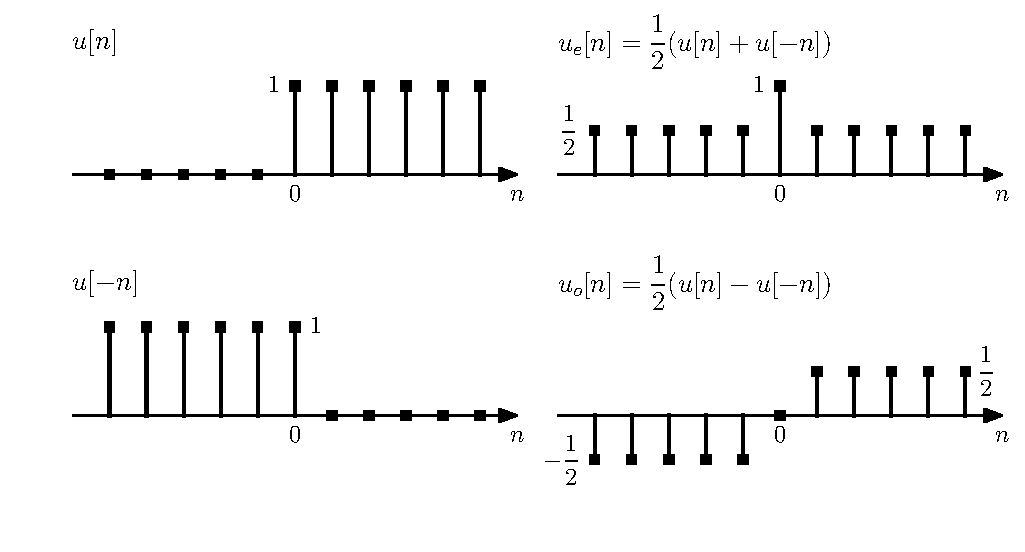
\includegraphics[width=0.85\textwidth]{figuras/seq_and_sys_step_dtft_computation.pdf}
 \caption{\label{fig:seq_and_sys_step_dtft_computation} Representación de la función escalón \(u[n]\) como la suma de la función par \(u_e[n]\) y la función impar \(u_o[n]\).}
 \end{center}
\end{figure} 
Por la propiedad de linealidad de la transformada de Fourier, se cumple que 
\begin{equation}\label{eq:seq_and_sys_dtft_step_even_odd_sum_example}
 U(e^{j\omega})=U_e(e^{j\omega})+U_o(e^{j\omega}), 
\end{equation}
donde 
\[
 u[n]\overset{\mathcal{F}}{\longleftrightarrow}U(e^{j\omega}),
 \qquad\qquad 
 u_e[n]\overset{\mathcal{F}}{\longleftrightarrow}U_e(e^{j\omega}),
 \qquad\qquad
 u_o[n]\overset{\mathcal{F}}{\longleftrightarrow}U_o(e^{j\omega}).
\]
Por un lado, del par de transformadas de una constante dada por la ecuación \ref{eq:seq_and_sys_constant_dtft_pair}, la transformada de Fourier de \(u_e[n]\) es
\begin{equation}\label{eq:seq_and_sys_dtft_step_even_example}
 U_e(e^{j\omega})=\pi\delta(\omega)+\frac{1}{2}
 \qquad\qquad\textrm{para}\qquad\qquad 
 -\pi<\omega<\pi.
\end{equation}
Para calcular la transformada de Fourier de \(u_o[n]\) se observa primero que 
\[
 u_o[n-1]=u[n-1]-\frac{1}{2}-\frac{1}{2}\delta[n-1],
\]
y por lo tanto,
\[
 u_o[n]-u_o[n-1]=\underbrace{u[n]-u[n-1]}_{\displaystyle\delta[n]}-\frac{1}{2}(\delta[n]-\delta[n-1])=
 \frac{1}{2}(\delta[n]+\delta[n-1]).
\]
Aplicando la transformada de Fourier en ambos lados de esta igualdad, considerando la propiedad de desplazamiento temporal de la DTFT en la sección \ref{sec:seq_and_sys_dtft_temporal_and freq_shift}, se deduce que 
\[
 U_o(e^{j\omega})-U_o(e^{j\omega})e^{-j\omega}=\frac{1+e^{-j\omega}}{2},
\]
es decir, 
\begin{equation}\label{eq:seq_and_sys_dtft_step_odd_example}
 U_o(e^{j\omega})=\frac{1+e^{-j\omega}}{2(1-e^{-j\omega})}. 
\end{equation}
Combinando los resultados de las ecuaciones \ref{eq:seq_and_sys_dtft_step_even_odd_sum_example}, \ref{eq:seq_and_sys_dtft_step_even_example} y \ref{eq:seq_and_sys_dtft_step_odd_example} resulta en que 
\[
 U(e^{j\omega})=\pi\delta(\omega)+\frac{1}{2}\left(1+\frac{1+e^{-j\omega}}{1-e^{-j\omega}}\right)
  =\pi\delta(\omega)+\frac{1}{1-e^{-j\omega}}.
\]
Se concluye que 
\begin{equation}\label{eq:seq_and_sys_step_dtft}
 u[n]\overset{\mathcal{F}}{\longleftrightarrow}\pi\delta(\omega)+\frac{1}{1-e^{-j\omega}}
 \qquad\qquad\textrm{para}\qquad\qquad 
 -\pi<\omega<\pi.
\end{equation}

\section{Señales aleatorias en tiempo discreto} 
 
Esta sección consiste en un resumen de conceptos básicos sobre señales aleatorias en tiempo discreto.
 
Una señal aleatoria se considera como un miembro de un conjunto de señales en tiempo discreto caracterizado por un conjunto de funciones de densidad de probabilidad. Cada muestra individual \(x[n]\) de una señal particular se asume ser la realización de una variable aleatoria \(\x_n\) subyacente. La señal completa es representada por una colección de dichas variables aleatorias, una por cada muestra \(-\infty<n<\infty\). Esta colección de variables aleatorias es referida como \emph{proceso aleatorio}, y se asume que una secuencia de muestras particular \(x[n]\) para \(-\infty<n<\infty\) h sido generada por el proceso aleatorio subyacente a la señal. Para describir completamente al proceso aleatorio se necesita especificar la distribuciones de probabilidad individuales y conjuntas de todas las variables aleatorias.

Considérese un sistema LTI estable con respuesta al impulso \(h[n]\) real, y sea \(x[n]\) la realización de un proceso aleatorio en tiempo discreto estacionario en sentido amplio. 
La salida del sistema lineal también es la realización de un proceso aleatorio vinculado a la salida mediante la transformación
\[
 y[n]=\sum_{k=-\infty}^\infty h[n-k]x[k]=\sum_{k=-\infty}^\infty h[k]x[n-k].
\]

La media de los procesos de entrada y salida son respectivamente
\[
 m_x[n]=E\{x[n]\}
 \qquad\qquad\textrm{y}\qquad\qquad
 m_y[n]=E\{y[n]\}.
\]
Como \(x[n]\) es estacionario,\footnote{De aquí en mas un proceso estacionario en sentido amplio será referido simplemente como estacionario.} \(m_x[n]\) es independiente de \(n\) y será denotado como \(m_x\). La media de la salida es
\[
 m_y[n]=E\{y[n]\}=\sum_{k=-\infty}^\infty h[k]E\{x[n-k]\}=m_x\sum_{k=-\infty}^\infty h[k],
\]
también constante. Observar que la media del proceso de salida puede expresarse en función de la respuesta en frecuencia del sistema como
\[
 m_y=H(e^{j0})m_x.
\]

La función de autocorrelación de la salida es
\begin{align*}
 \phi_{yy}[n,\,n+m]&=E\{y[n]y[n+m]\}\\
   &=E\left\{\sum_{k=-\infty}^\infty h[k]x[n-k]\sum_{r=-\infty}^\infty h[r]x[n+m-r]\right\}\\
   &=\sum_{k=-\infty}^\infty h[k]\sum_{r=-\infty}^\infty h[r]E\{x[n-k]x[n+m-r]\}.
\end{align*}
Considerando que como \(x[n]\) es estacionario, se cumple que \(E\{x[n-k]x[n+m-r]\}=\phi_{xx}[m+k-r]\) depende solo de la diferencia temporal \(m+k-r\), y por o tanto
\begin{equation}\label{eq:seq_and_sys_random_lti_output_autocorrelation}
 \phi_{yy}[n,\,n+m]=\sum_{k=-\infty}^\infty h[k]\sum_{r=-\infty}^\infty h[r]\phi_{xx}[m+k-r]=\phi_{yy}[m], 
\end{equation}
es decir, la autocorrelación de la salida también depende solo de la diferencia temporal \(m\). Se concluye que la salida de un sistema LTI cuando la entrada es un proceso estacionario en sentido amplio es también un proceso estacionario en sentido amplio.
 
Realizando la sustitución \(l=r-k\), la ecuación \ref{eq:seq_and_sys_random_lti_output_autocorrelation} puede escribirse como
\begin{align}
 \phi_{yy}[m]&=\sum_{k=-\infty}^\infty h[k]\sum_{l=-\infty}^\infty h[l+k]\phi_{xx}[m-l]\nonumber\\
   &=\sum_{l=-\infty}^\infty\phi_{xx}[m-l]\sum_{k=-\infty}^\infty h[k]h[l+k]\nonumber\\
   &=\sum_{l=-\infty}^\infty\phi_{xx}[m-l]c_{hh}[l],\label{eq:seq_and_sys_random_lti_output_autocorrelation_convolution}
\end{align}
donde se definió
\begin{equation}\label{eq:seq_and_sys_random_lti_deterministic_autocorrelation}
 c_{hh}[l]=\sum_{k=-\infty}^\infty h[k]h[l+k]\overset{(a)}{=}\sum_{m=-\infty}^\infty h[m-l]h[m]=h[l]*h[-l], 
\end{equation}
donde en \((a)\) se realizó el cambio de variable \(m=l+k\). La secuencia \(c_{hh}[l]\) es referida como \emph{secuencia de autocorrelación determinística} de \(h[n]\). La ecuación \ref{eq:seq_and_sys_random_lti_output_autocorrelation_convolution} indica que la autocorrelación de la salida de un sistema lineal es la convolución entre la autocorrelación de la entrada y la autocorrelación determinística de la respuesta al impulso del sistema.
 
Si \(\Phi_{xx}(e^{j\omega})\), \(\Phi_{yy}(e^{j\omega})\) y \(C_{hh}(e^{j\omega})\) son las transformadas de Fourier de \(\phi_{xx}[m]\), \(\phi_{yy}[m]\) y \(c_{hh}[l]\) respectivamente, al tomar la transformada de Fourier de la ecuación \ref{eq:seq_and_sys_random_lti_output_autocorrelation_convolution}, se obtiene que 
\[
 \Phi_{yy}(e^{j\omega})=C_{hh}(e^{j\omega})\Phi_{xx}(e^{j\omega}),
\]
y al tomar la transformada de Fourier en la ecuación \ref{eq:seq_and_sys_random_lti_deterministic_autocorrelation}, resulta en que 
\[
 C_{hh}(e^{j\omega})=H(e^{j\omega})H^*(e^{j\omega})=|H(e^{j\omega})|^2,
\]
y por lo tanto,
\[
 \Phi_{yy}(e^{j\omega})=|H(e^{j\omega})|^2\Phi_{xx}(e^{j\omega}),
\]
Esta ecuación brinda la motivación del término \emph{densidad espectral de potencia}. Específicamente,
\[
 E\{y^2[n]\}=\phi_{yy}[0]=\frac{1}{2\pi}\int_{-\pi}^\pi\Phi_{yy}(e^{j\omega})\,d\omega, 
\]
que es la potencia promedio de la salida. Puede probarse que la función densidad espectral de potencia de una señal real es una función par, real y no negativa.

Otro resultado importante es sobre la correlación cruzada entre la entrada y la salida de un sistema LTI,
\begin{align*}
 \phi_{yx}[m]&=E\{x[n]y[n+m]\}\\
   &=E\left\{x[n]\sum_{k=-\infty}^\infty h[k]x[n+m-k]\right\}\\
   &=\sum_{k=-\infty}^\infty h[k]E\left\{x[n]x[n+m-k]\right\}\\
   &=\sum_{k=-\infty}^\infty h[k]\phi_{xx}[m-k].
\end{align*}
Se observa que la correlación cruzada entre la entrada y la salida es la convolución entre la respuesta al impulso y la autocorrelación de la entrada. Aplicando la transformada de Fourier se obtiene que 
\[
 \Phi_{yx}(e^{j\omega})=H(e^{j\omega})\Phi_{xx}(e^{j\omega}).
\]

\chapter{La transformada \texorpdfstring{\(z\)}{z}}\label{ch:z_transform}

\section{La transformada \texorpdfstring{\(z\)}{z}}

La transformada \(z\) de una secuencia \(x[n]\) se define como
\begin{equation}\label{eq:z_transform_definition}
 X(z)=\sum_{n=-\infty}^\infty x[n]z^{-n}. 
\end{equation}
Comparando esta definición con la definición \ref{eq:seq_and_sys_dtft_definition} de la transformada de Fourier es evidente que hay una relación cercana entre ambas transformadas. En particular, si se reemplaza la variable compleja \(z\) en la ecuación \ref{eq:z_transform_definition} por el valor complejo \(e^{j\omega}\), la transformada \(z\) se reduce a la transformada de Fourier. De hecho, esa es la motivación para la notación \(X(e^{j\omega})\) de la transformada de Fourier. Mas en general, expresando \(z\) en coordenadas polares como
\[
 z=re^{j\omega},
\]
la ecuación \ref{eq:z_transform_definition} queda
\[
 X(re^{j\omega})=\sum_{n=-\infty}^\infty x[n](re^{-j\omega})^{-n},
\]
o
\begin{equation}\label{eq:z_transform_definition_polar}
 X(re^{j\omega})=\sum_{n=-\infty}^\infty(x[n]r^{-n})e^{-j\omega n}, 
\end{equation}
que es la transformada de Fourier de la secuencia \(x[n]r^{-n}\). Con \(r=1\), la ecuación \ref{eq:z_transform_definition_polar} se reduce a la transformada de Fourier de \(x[n]\). En el plano complejo \(z\), el contorno \(z=e^{j\omega}\) o \(|z|=1\) es una circunferencia de radio unidad y es referida como \emph{circunferencia unidad}. La transformada \(z\) evaluada en la circunferencia unidad corresponde a la transformada de Fourier.

Como se discutió en la capítulo \ref{ch:signals_and_systems}, la representación en series de potencias de la transformada de Fourier no converge para todas las secuencias. De forma similar, la transformada \(z\) no converge para todas las secuencias o para todos los valores de \(z\). Para una secuencia dada, el conjunto de valores de \(z\) para los cuales la serie de potencias de la transformada \(z\) converge se llama \emph{región de convergencia} (\emph{ROC}, region of convergence) de la transformada \(z\). Como se estableció en la sección \ref{sec:fourier_transform_representation}, si la secuencia es absolutamente sumable, la transformada de Fourier converge a una función continua de \(\omega\). Este criterio aplicado en la ecuación \ref{eq:z_transform_definition_polar} conduce a la condición
\[
 |X(re^{j\omega})|\leq\sum_{n=-\infty}^\infty|x[n]r^{-n}|<\infty 
\]
para la convergencia de la transformada \(z\). Debido a la multiplicación de la secuencia por la exponencial real \(r^{-n}\), es posible que la transformada \(z\) converja incluso aunque la transformada de Fourier (\(r=1\)) no lo haga. Por ejemplo, la secuencia \(u[n]\) no es absolutamente sumable y por lo tanto, la tranformada de Fourier no converge absolutamente (ver el ejemplo al final de la sección \ref{sec:fourier_transform_theorems}). Sin embargo, la secuencia \(u[n]r^{-n}\) es absolutamente sumable si \(r>1\), lo que significa que la transformada \(z\) existe con ROC \(r=|z|>1\).

La convergencia de la serie de potencias \ref{eq:z_transform_definition} depende únicamente de \(|z|\), ya que \(|X(z)|<\infty\) si
\[
 \sum_{n=-\infty}^\infty|x[n]||z|^{-n}<\infty,
\]
es decir, la ROC consiste en todos los valores de \(z\) en donde esta ecuación se cumple. Por lo tanto, si cierto valor \(z_1\) pertenece a la ROC, todos los valores de \(z\) definidos en el círculo \(|z|=|z_1|\) pertenecen a la ROC. Una consecuencia de esto es que la ROC consiste en un anillo en el plano \(z\) centrado en el origen. Su frontera exterior será un círculo o puede extenderse por el exterior hasta el infinito, y su frontera interior será un círculo o puede extenderse hacia el interior hasta contener el origen. Si la ROC incluye la circunferencia unidad, es decir, si la transformada \(z\) converge para \(|z|=1\), la transformada de Fourier de la secuencia converge. Por el contrario, si la ROC no incluye la cirunferencia unidad, la transformada de Fourier de la secuencia no converge absolutamente.

Una serie de potencias de la forma de la ecuación \ref{eq:z_transform_definition} es una serie de Laurent. Por lo tanto, existen una cantidad de teoremas elegantes y poderosos de la teoría de funciones de variable compleja que pueden emplearse en el estudio de la transformada \(z\) (ver \cite{brown2013complex}, por ejemplo). Por ejemplo, una serie de Laurent, y por lo tanto una transformada \(z\), representa una función analítica en cada punto de la ROC. En consecuencia, la transformada \(z\) y todas sus derivadas deben ser funciones continuas en \(z\) dentro de la ROC. Esto implica que si la ROC incluye la circunferencia unidad, la transformada de Fourier y todas sus derivadas respecto a \(\omega\) deben ser funciones continuas de \(\omega\). Además, de la discusión de la sección \ref{sec:fourier_transform_representation}, la secuencia debe ser absolutamente sumable o estable.

La transformada \(z\) es especialmente útil cuando la suma infinita puede expresarse de forma cerrada. Entre las transformadas \(z\) más importantes y útiles están las que \(X(z)\) es una función racional dentro de la ROC, es decir,
\[
 X(z)=\frac{P(z)}{Q(z)},
\]
donde \(P(z)\) y \(Q(z)\) son polinomios en \(z\). En general, los valores de \(z\) para los cuales \(X(z)=0\) son los \emph{ceros} de \(X(z)\) y los valores de \(z\) para los cuales \(X(z)\) es infinito son los \emph{polos} de \(z\). En el caso de las funciones racionales, los ceros son las raíces del polinomio del numerador y los polos son las raíces del polinomio del denominador. Para transformadas \(z\) racionales existe una relación importante entre la ubicación de los polos de \(X(z)\) y la ROC de la transformada \(z\).

\paragraph{Ejemplo: secuencia exponencial de largo finito} Se considera la señal
\[
 x[n]=
 \left\{
 \begin{array}{ll}
  a^n, & 0\leq n\leq N-1\\
  0, & \textrm{en otro caso.}
 \end{array}
 \right.
\]
La transformada \(z\) es
\[
 X(z)=\sum_{n=0}^{N-1}a^nz^{-n}=\sum_{n=0}^{N-1}(az^{-1})^n=\frac{1-(az^{-1})^N}{1-az^{-1}}
  =\frac{1}{z^{N-1}}\,\frac{z^N-a^N}{z-a}.
\]
La ROC está determinada por los valores de \(z\) para los cuales
\[
 \sum_{n=0}^{N-1}|az^{-1}|^n<\infty
\]
Como la cantidad de sumandos es finita, la suma es finita siempre que \(az^{-1}\) sea finito. Asumiendo que \(a\) es finito, \(az^{-1}\) es finito salvo en \(z=0\). Por lo tanto, la ROC consiste en el plano complejo completo excepto el origen \(z=0\). Para encontrar los ceros y polos de la transformada \(z\) se observa que las raíces del numerador son
\[
 z^N-a^N=0
 \qquad\Rightarrow\qquad
 z^N=a^Ne^{j2\pi k}
 \qquad\Rightarrow\qquad
 z_k=ae^{j2\pi k/N},\qquad 
 k=0,\,1,\,\dots,\,N-1.
\]
El cero en \(z=a\) correspondiente a \(k=0\) se cancela con el polo en \(z=a\). En consecuencia, los únicos polos son los \(N-1\) en el origen y los \(N-1\) ceros están en
\[
 z_k=ae^{j2\pi k/N},\qquad 
 k=1,\,\dots,\,N-1.
\]
En la figura \ref{fig:example_3_6_zero_pole_plot} se muestra el diagrama de polos y ceros de este ejemplo para el caso en que \(N=16\) y \(0<a<1\) real.
\begin{figure}[!htb]
  \begin{minipage}[c]{0.42\textwidth}
    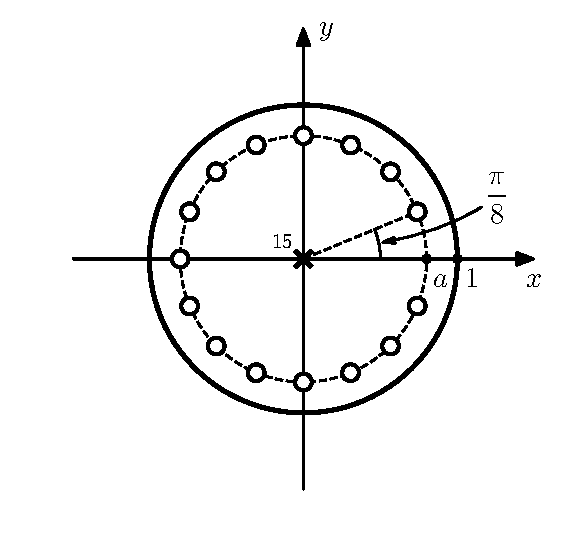
\includegraphics[width=\textwidth]{figuras/example_3_6_zero_pole_plot.pdf}
  \end{minipage}\hfill
  \begin{minipage}[c]{0.48\textwidth}
    \caption{
      Diagrama de polos y ceros en el plano complejo \(z=x+iy\) para \(N=16\) y \(0<a<1\) real. La ROC consiste en todo el plano complejo excepto \(z=0\).
    }\label{fig:example_3_6_zero_pole_plot}
  \end{minipage}
\end{figure}

\section{Propiedades de la ROC de la transformada \texorpdfstring{\(z\)}{z}}

En esta sección se resumen las propiedades de la transformada \(z\).
\begin{enumerate}
 \item La ROC es un anillo o un disco centrado en el origen, es decir,
\[
  0\leq r_R \leq |z| \leq r_L \leq \infty.
\]
\item La transformada de Fourier converge absolutamente si y solo si la ROC incluye la circunferencia unidad.
\item La ROC no puede contener ningún polo.
\item Si \(x[n]\) es una \emph{secuencia de duración finita} la ROC es todo el plano complejo excepto tal vez \(z=0\) o \(z=\infty\).
\item Si \(x[n]\) es una \emph{secuencia hacia adelante}, la ROC se extiende desde el polo de mayor magnitud hasta infinito.
\item Si \(x[n]\) es una \emph{secuencia hacia atrás}, la ROC se extiende desde el polo de menor magnitud hasta el origen del plano complejo.
\item Si \(x[n]\) es una \emph{secuencia hacia ambos lados}, la ROC consiste en un anillo, cuyas fronteras interior y exterior están acotadas por polos.
\item La ROC debe ser una región conexa.
\end{enumerate}

Para especificar completamente a la transformada \(z\) de una secuencia no alcanza únicamente con la expresión algebraica o el diagrama de polos y ceros, se necesita además especificar la ROC. Las propiedades consideradas en esta sección limitan las posibles ROC asociadas a determinado patrón de polos y ceros. Para ilustrar esto, considérese el diagrama de polos y ceros mostrado en la figura \ref{fig:z_transform_roc_posibilities}. De las propiedades 1, 3 y 8, se deduce que hay solo cuatro posibilidades de ROC, las cuales se muestran en la figura. Si se asume que la circunferencia unidad está entre los polos en \(z=b\) y \(z=c\), es decir, \(b<1<c\), la secuencia correspondiente a la ROC que consiste en el anillo \(b<|z|<c\) es la única cuya transformada de Fourier converge.
\begin{figure}[!htb]
 \begin{center}
 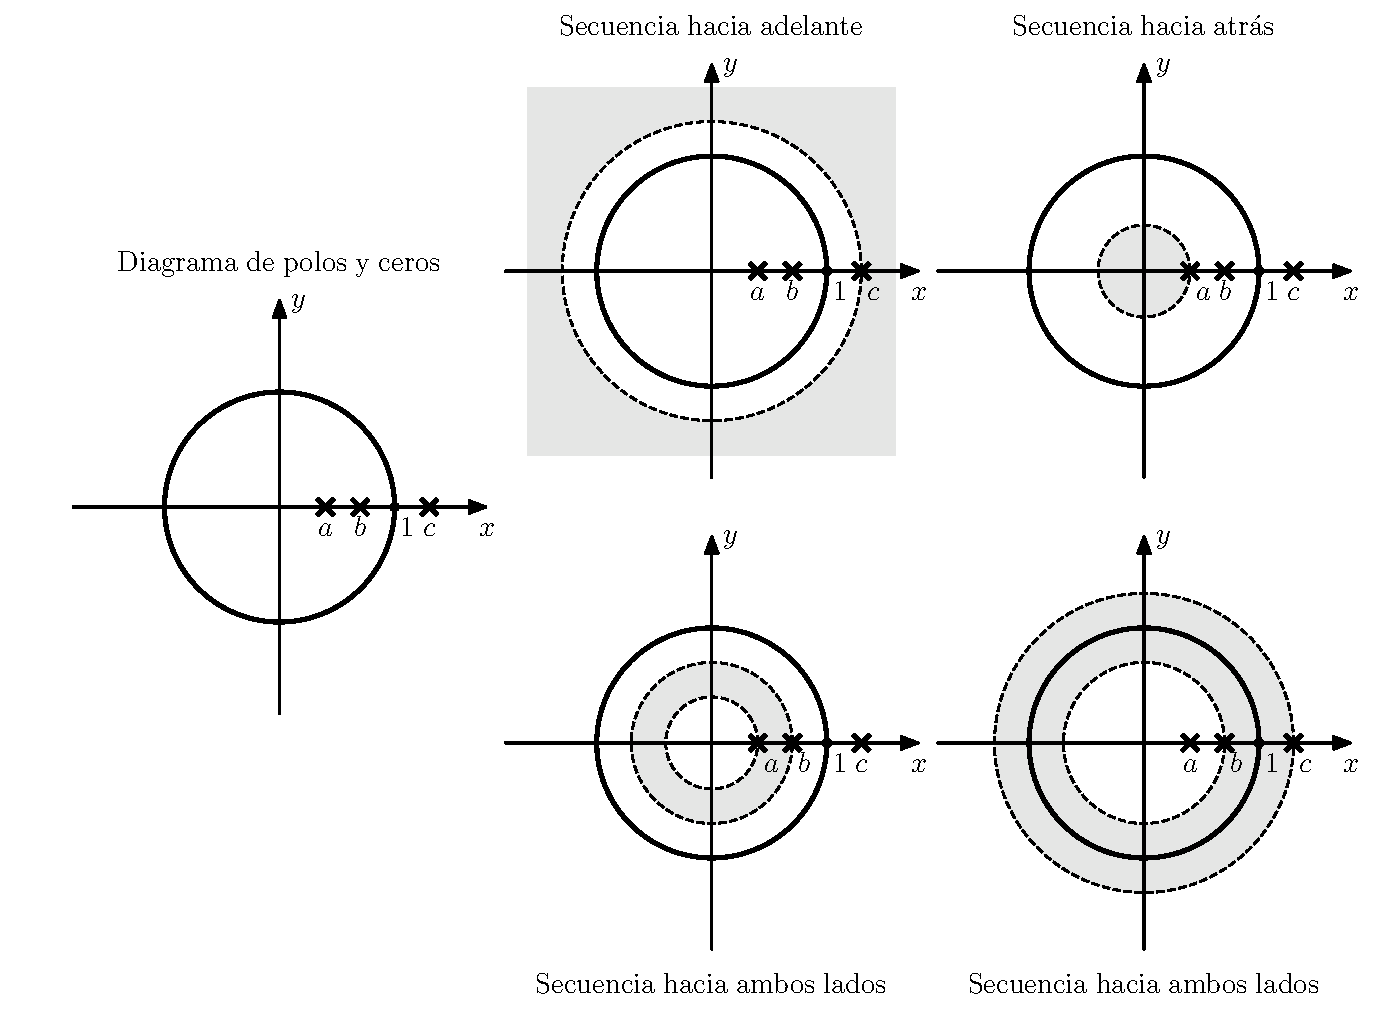
\includegraphics[width=1\textwidth]{figuras/z_transform_roc_posibilities.pdf}
 \caption{\label{fig:z_transform_roc_posibilities} Diagrama de polos y ceros de una transformada \(z\) y las posibles ROC. Una corresponde a una secuencia hacia adelante, otra a una secuencia hacia atrás y dos a secuencias hacia ambos lados distintas.}
 \end{center}
\end{figure}

\section{La transformada \texorpdfstring{\(z\)}{z} inversa} 
 
En el empleo de la transformada \(z\) para el análisis de secuencias en tiempo discreto debe ser posible el pasaje entre las representaciones en el dominio del tiempo y en el dominio \(z\). A menudo, este análisis implica calcular la transformada \(z\) y luego de algo de manipulación de las expresiones algebraicas, calcular la transformada \(z\) inversa. La transformada \(z\) inversa es la integral de contorno
\begin{equation}\label{eq:z_transform_inverse_computation}
 x[n]=\frac{1}{2\pi j}\oint_C X(z)z^{n-1}, 
\end{equation}
donde \(C\) es un contorno cerrado orientado en sentido antihorario dentro de la ROC que encierra al origen. Esta expresión se deriva del teorema integral de Cauchy de la teoría de funciones de variable compleja. Específicamente, \(x[n]\) son los coeficientes de la representación en series de Laurent de la función \(X(z)\) (ver la sección 66 de \cite{brown2013complex} sobre la representación en series de Laurent de una función de variable compleja, y también el ejercicio 8 de la sección 68). Sin embargo, para el tipo de secuencias y transformadas \(z\) encontradas en el análisis de sistemas LTI, procedimientos menos formales son suficientes y preferibles para la evaluación de la ecuación  \ref{eq:z_transform_inverse_computation}. En las secciones siguientes se consideran dichos procedimientos, en particular, el método de inspección, la expansión en fracciones simples y la expansión en series de potencia.

\subsection{Método de inspección}

El método de inspección consiste reconocer mediante inspección pares de transformadas mediante el uso de una tabla de pares de transformadas básicos, como la que se muestra en el cuadro \ref{tab:z_transform_pairs}.
\begin{table}[ht!]
\begin{center}
\begin{tabular}{ccc}\hline
Secuencia, \(x[n]\) & Transformada \(Z\), \(X(z)\) & ROC \\ \hline
\(\delta[n]\)  &  1  & \(\forall z\) \\[\bigskipamount]
\(\delta[n-n_0]\) & 	\(z^{-n_0}\) & \(z \neq 0\textrm{ o }z\neq\infty\)\\[\bigskipamount]
\(a^n u[n]\)   &  \(\dfrac{1}{1-a z^{-1}}\) & \(|z| > |a|\)\\[\bigskipamount]
\(-a^n u[-n-1]\)  &  \(\dfrac{1}{1-a z^{-1}}\)   & \(|z| < |a|\)\\[\bigskipamount]
\(n u[n]\)  & \(\dfrac{z^{-1}}{( 1-z^{-1} )^2}\)  &  \(|z| > 1\)\\[\bigskipamount]
\(- n u[-n-1]\)  &  \(\dfrac{z^{-1} }{ (1 - z^{-1})^2 }\)  & \(|z| < 1\)\\[\bigskipamount]
\(n^2 u[n]\)  & \(\dfrac{ z^{-1} (1 + z^{-1} )}{(1 - z^{-1})^3}\) &  \(|z| > 1\)\\[\bigskipamount]
\(-n^2 u[-n - 1]\)  &  \(\dfrac{ z^{-1} (1 + z^{-1} )}{(1 - z^{-1})^3}\) & \(|z| < 1\)\\[\bigskipamount]
\(\cos(\omega_0 n) u[n]\)  & \(\dfrac{ 1-z^{-1} \cos(\omega_0)}{ 1-2z^{-1}\cos(\omega_0)+ z^{-2}}\) & \(|z| >1\)\\[\bigskipamount]
\(\sin(\omega_0 n) u[n]\) & \(\dfrac{ z^{-1} \sin(\omega_0)}{ 1-2z^{-1}\cos(\omega_0)+ z^{-2}}\) & \(|z| >1\)\\[\bigskipamount]
\(a^n \cos(\omega_0 n) u[n]\)  & \(\dfrac{1-a z^{-1} \cos( \omega_0)}{1-2az^{-1}\cos(\omega_0)+ a^2 z^{-2}}\)  & \(|z|>|a|\)\\[\bigskipamount]
\(a^n \sin(\omega_0 n) u[n]\) & \(\dfrac{ az^{-1} \sin(\omega_0) }{ 1-2az^{-1}\cos(\omega_0)+ a^2 z^{-2}}\) & \(|z|>|a|\)
\end{tabular}
\end{center}\caption{Pares de transformadas \(z\) básicos.}\label{tab:z_transform_pairs}
\end{table}
Por ejemplo, si se necesita encontrar la transformada \(z\) inversa de 
\[
 X(z)=\frac{1}{1-\frac{1}{2}z^{-1}},
 \qquad
 |z|>\frac{1}{2},
\]
del cuadro se observa que 
\[
 a^nu[n]\;\overset{\mathcal{Z}}{\longleftrightarrow}\;\frac{1}{1-az^{-1}},
 \qquad
 |z|>a,
\]
y por lo tanto,
\[
 x[n]=\left(\frac{1}{2}\right)^nu[n].
\]

Si una transformada \(z\) dada puede expresarse como suma de términos que se encuentran en una tabla de transformadas, su transformada inversa puede encontrarse solo empleando la tabla. Esto está vinculado la método de fracciones simples descripto en la siguiente sección. 
 
\subsection{Método de fracciones simples} 
 
Como se describió, las transformadas \(z\) pueden encontrarse mediante inspección si la expresión de la transformada \(z\) está tabulada. A veces, \(X(z)\) no se encuentra explícitamente en una tabla, pero puede descomponerse como la suma de términos mas simples, cada uno de los cuales están tabulados. Este es el caso de las funciones racionales, que pueden expandirse en fracciones simples en términos que están tabulados. 

Para ver como se obtiene la expansión en fracciones simples se asume que \(X(z)\) se puede expresar como un cociente de polinomios en \(z^{-1}\) de la siguiente forma:
\begin{equation}\label{eq:z_transform_rational_function_generic}
 X(z)=\dfrac{\sum\limits_{k=0}^Mb_kz^{-k}}{\sum\limits_{k=0}^Na_kz^{-k}}. 
\end{equation}
Una expresión equivalente como cociente de polinomios en \(z\) es
\[
 X(z)=\dfrac{z^N\sum\limits_{k=0}^Mb_kz^{M-k}}{z^M\sum\limits_{k=0}^Na_kz^{N-k}}.
\]
Esta expresión muestra que hay explícitamente \(M\) ceros y \(N\) polos distintos de cero asumiendo que \(a_0\), \(b_0\), \(a_N\) y \(b_M\) son no nulos. Además hay \(M-N\) polos en \(z=0\) si \(M>N\) o \(N-M\) ceros en \(z=0\) si \(N>M\). Esto indica que en cualquier caso, las transformadas \(z\) de la forma de la ecuación \ref{eq:z_transform_rational_function_generic} tienen la misma cantidad de polos y ceros en el plano complejo finito, y no hay polos o ceros en \(z=\infty\). Para obtener la expansión en fracciones simples de \(X(z)\) de la ecuación \ref{eq:z_transform_rational_function_generic}, es mas conveniente factorizar el numerador y el denominador en monomios,
\begin{equation}\label{eq:z_transform_rational_function_factorized}
 X(z)=\frac{b_0\prod\limits_{k=1}^M(1-c_kz^{-1})}{a_0\prod\limits_{k=1}^N(1-d_kz^{-1})}, 
\end{equation}
donde \(c_k\) y \(d_k\) son las raíces de numerador y denominador respectivamente. Se distinguen tres casos:
\begin{enumerate}
 \item \(M<N\) y todos los polos son de primer orden. En este caso, \(X(z)\) puede expresarse como
 \begin{equation}\label{eq:z_transform_rational_function_simple_fractions_1}
  X(z)=\sum_{k=1}^N\frac{A_k}{1-d_kz^{-1}}.  
 \end{equation}
 Observar que el numerador que resulta al sumar los términos es a lo sumo de grado \(N-1\) en \(z^{-1}\).
 Los parámetros \(A_k\) pueden calcularse sacando denominador común en los sumandos del lado derecho de la igualdad y luego igualando los coeficientes de los polinomios del numerados en ambos lados de la igualdad. Esto conduce a un sistema de \(N\) ecuaciones donde los parámetros \(A_k\) son las \(N\) incógnitas. Una forma mas directa de obtener los parámetros \(A_k\) es multiplicando ambos lados de la ecuación \ref{eq:z_transform_rational_function_simple_fractions_1} por \((1-d_kz^{-1})\) y luego evaluando en \(z=d_k\), es decir,
 \begin{equation}\label{eq:z_transform_rational_function_simple_fractions_A_k}
  A_k=(1-d_kz^{-1})X(z)\big|_{z=d_k}.  
 \end{equation}
 \item \(M\geq N\) y todos los polos son de primer orden. En este caso debe sumarse un polinomio de grado \(M-N\) en el lado derecho de la ecuación \ref{eq:z_transform_rational_function_simple_fractions_1},
 \begin{equation}\label{eq:z_transform_rational_function_simple_fractions_2}
  X(z)=\sum_{r=0}^{M-N}B_rz^{-r}+\sum_{k=1}^N\frac{A_k}{1-d_kz^{-1}}.  
 \end{equation}
 Los coeficientes \(B_r\) pueden obtenerse mediante división larga del numerador entre el denominador, donde el proceso de división finaliza cuando el resto es de menor grado que el denominador. Los coeficientes \(A_k\) pueden obtenerse igual que antes mediante la ecuación \ref{eq:z_transform_rational_function_simple_fractions_A_k}.
 \item \(M\geq N\) y existen polos de orden múltiple. Si \(X(z)\) tiene un polo de orden \(s\) en \(z=d_i\) y el resto de los polos son de primer orden, la ecuación \ref{eq:z_transform_rational_function_simple_fractions_2} se convierte en
 \begin{equation}\label{eq:z_transform_rational_function_simple_fractions_3}
  X(z)=\sum_{r=0}^{M-N}B_rz^{-r}+\sum_{k=1,\,k\neq i}^N\frac{A_k}{1-d_kz^{-1}}+\sum_{m=1}^s\frac{C_m}{(1-d_iz^{-1})^m}.  
 \end{equation}
 Los coeficientes \(A_k\) y \(B_r\) se obtienen como antes. Los coeficientes \(C_m\) se obtienen de la ecuación
 \[
  C_m=\frac{1}{(s-m)!(-d_i)^{s-m}}\left\{\frac{d^{s-m}}{dw^{s-m}}\left[(1-d_iw)^sX(w^{-1})\right]\right\}_{w=d_i^{-1}}.
 \]
\end{enumerate}

La ecuación \ref{eq:z_transform_rational_function_simple_fractions_3} es la forma mas general de la expansión en funciones simples de una transformada \(z\) racional expresada como función de \(z^{-1}\) para el caso en que \(M\geq N\) y \(d_i\) es un polo múltiple de orden \(s\). Si hay mas de un polo múltiple, la ecuación \ref{eq:z_transform_rational_function_simple_fractions_3} tendrá un término como el tercer sumando por cada polo múltiple. Si el grado \(M\) del numerador es menor al grado \(N\) del denominador, el término polinómico en la ecuación \ref{eq:z_transform_rational_function_simple_fractions_3} desaparece.
 
\subsection{Expansión en series de potencias} 
 
La expresión de la definición de la transformada \(z\) es una serie de Laurent donde los valores \(x[n]\) de la secuencia son los coeficientes de \(z^{-n}\). Por lo tanto, si la transformada \(z\) está dada como una serie de potencias de la forma
\begin{equation}\label{eq:z_transform_definition_2}
 \begin{aligned}
  X(z)&=\sum_{n=-\infty}^\infty x[n]z^{-n}\\
  &=\cdots+x[-2]z^2+x[-1]z+x[0]+x[1]z^{-1}+x[2]z^{-2}+\cdots,
 \end{aligned}
\end{equation}
se puede determinar cualquier valor de la secuencia encontrando el coeficiente de la serie de Laurent de la potencia apropiada de \(z^{-1}\) (ver el capítulo 5 de \cite{brown2013complex}). Este enfoque ya se empleó en encontrar la  parte polinómica de la expansión en fracciones simples cuando \(M\geq N\).

\paragraph{Ejemplo: transformada inversa mediante expansión en series de potencias} Se considera la transformada \(z\) 
\[
 X(z)=\log(1+az^{-1})
 \qquad\qquad\textrm{cuando}\qquad\qquad
 |z|>|a|.
\]
Empleando la expansión en series de Taylor conocida
\[
 \log z=\sum_{n=1}^\infty\frac{(-1)^{n+1}}{n}(z-1)^n
 \qquad\qquad\textrm{cuando}\qquad\qquad
 |z-1|<1,
\]
(ver el ejercicio 6 de la sección 72 de \cite{brown2013complex}), al reemplazar \(z\) por \(1+az^{-1}\) en esta expresión se obtiene la representación en series de Laurent
\[
 \log(1+az^{-1})=\sum_{n=1}^\infty\frac{(-1)^{n+1}}{n}a^nz^{-n}
 \qquad\qquad\textrm{cuando}\qquad\qquad
 |az^{-1}|<1
 \qquad\qquad\textrm{o}\qquad\qquad
 |z|>|a|.
\]
Comparando esta expresión con la definición \ref{eq:z_transform_definition_2} de la transformada \(z\), se deduce que la antitransformada \(z\) es 
\[
 x[n]=
 \left\{
 \begin{array}{ll}
  (-1)^{n+1}\dfrac{a^n}{n}, & n\geq1\\[\medskipamount]
  0, & n\leq0.
 \end{array}
 \right.
\]

\paragraph{Ejemplo: antitransformada \(z\) correspondiente a la secuencia exponencial}

Sea la transformada \(z\)
\[
 X(z)=\frac{1}{1-az^{-1}},
\]
que tiene un polo en \(z=a\). Se quiere encontrar las secuencias correspondientes a las regiones de convergencia
\(|z|>|a|\) y \(|z|<|a|\). Para hacerlo se calculará la expansión en series de Laurent de \(X(z)\). Un resultado conocido de la teoría de análisis complejo es que la siguiente expansión en series de Laurent:
\begin{equation}\label{eq:z_transform_exponential_z_transform}
 \frac{1}{1-z}=\sum_{n=0}^\infty z^n=1+z+z^2+\cdots
 \qquad\qquad\textrm{cuando}\qquad\qquad
 |z|<1, 
\end{equation}
identidad mostrada en el ejemplo de la sección 61 y en el ejemplo 1 de la sección 64 de \cite{brown2013complex}. Reemplazando \(z\) por \(az^{-1}\) en esta identidad conduce a la expansión en series de Laurent
\[
 \frac{1}{1-az^{-1}}=\sum_{n=0}^\infty a^nz^{-n}
 \qquad\qquad\textrm{cuando}\qquad\qquad
 |az^{-1}|<1
 \qquad\qquad\textrm{o}\qquad\qquad
 |z|>|a|.
\]
Comparando este resultado con la ecuación \ref{eq:z_transform_definition_2}, se deduce que la antitransformada \(z\) cuando \(|z|>|a|\) es
\[
 x[n]=a^nu[n].
\]
Por otro lado, se tiene que
\begin{equation}\label{eq:z_transform_exponential_anticausal}
 X(z)=\frac{1}{1-az^{-1}}=\frac{a^{-1}z}{a^{-1}z(1-az^{-1})}=-a^{-1}z\left(\frac{1}{1-a^{-1}z}\right). 
\end{equation}
Además, reemplazando \(z\) por \(a^{-1}z\) en la series de potencias \ref{eq:z_transform_exponential_z_transform} se obtiene la expansión en series de potencias
\[
 \frac{1}{1-a^{-1}z}=\sum_{n=0}^\infty a^{-n}z^n
 \qquad\qquad\textrm{cuando}\qquad\qquad
 |a^{-1}z|<1
 \qquad\qquad\textrm{o}\qquad\qquad
 |z|<|a|.
\]
Combinando ambos resultados, se obtiene la expansión en series de Laurent
\[
 \frac{1}{1-az^{-1}}=-a^{-1}z\sum_{n=0}^\infty a^{-n}z^n=-\sum_{n=0}^\infty a^{-(n+1)}z^{n+1}
  \overset{(a)}{=}-\sum_{m=-\infty}^{-1} a^mz^{-m}
  \quad\qquad\textrm{cuando}\quad\qquad
  |z|<|a|,
\]
donde en \((a)\) se realizó el cambio de variable \(m=-(n+1)\). Comparando este resultado con la ecuación \ref{eq:z_transform_definition_2}, se obtiene que la antitransformada \(z\) cuando \(|z|<|a|\) es
\[
 x[n]=-a^nu[-n-1].
\]
Observar que la expansión en series de potencias puede obtenerse mediante división larga (ver la sección 73 de \cite{brown2013complex}). Efectivamente, con 
\[
 X(z)=\frac{1}{1-az^{-1}}
 \qquad\qquad\textrm{cuando}\qquad\qquad
 |z|>|a|,
\]
la división larga conduce a  
\[
%\setlength\arraycolsep{0pt} 
\setlength\extrarowheight{10pt}
\begin{array}[t]{ccccc}
                       & 1 & +az^{-1} & +a^2z^{-2} & +\cdots\\[\medskipamount]
\cline{2-5}
1-az^{-1} 
                \bigg) & 1  &   &  &\\
                       & 1  & -az^{-1} &  & \\[\medskipamount]
\cline{2-5}
                       &    & az^{-1} &   & \\
                       &    & az^{-1} &  -a^2z^{-2} & \\[\medskipamount]
\cline{3-5}
                       &    &         &  a^2z^{-2} & \\
                       &    &         &  a^2z^{-2} & -a^3z^{-3} \\[\medskipamount]
\cline{4-5}
                       &    &                  &   & a^3z^{-3}\\
                       &    &                  &   & \vdots\\
\end{array}
\] 
es decir,
\[
 \frac{1}{1-az^{-1}}=\sum_{n=0}^\infty a^nz^{-n}
 \qquad\qquad\textrm{cuando}\qquad\qquad
 |z|>|a|.
\]
Dividiendo la mayor potencia de \(z^{-1}\) en el denominador entre la mayor potencia de \(z^{-1}\) en el numerador, se obtiene una expansión en series de potencias en \(z^{-1}\). Para el caso en que la ROC es \(|z|<|a|\) hay que expresar los polinomios del numerador y el denominador en potencias de \(z\), como en la ecuación \ref{eq:z_transform_exponential_anticausal}, y luego dividir. De esta forma se obtiene una expresión en series de potencias en \(z\) correspondiente a una secuencia hacia la izquierda.

\section{Propiedades de la transformada \texorpdfstring{\(z\)}{z}}\label{sec:z_transform_properties}
 
En la siguiente discusión, \(X(z)\) denota la transformada \(z\) de \(x[n]\) y \(R_x\) denota la ROC de \(X(z)\).

\subsection{Linealidad} 
 
La propiedad de linealidad establece que 
\[
 ax_1[n]+bx_2[n]\;\overset{\mathcal{Z}}{\longleftrightarrow}\;aX_1(z)+bX_2(z),
 \qquad\qquad\textrm{ROC contiene }R_{x_1}\cap R_{x_2}.
\]
Para el caso de secuencias con transformada \(z\) racional, si \(aX_1(z)+bX_2(z)\) tiene todos los polos de \(X_1(z)\) y \(X_2(z)\), es decir, no hay cancelación de polos y ceros, la ROC es la intersección de las ROCs individuales. Si en la combinación lineal se introducen ceros que se cancelan con polos, la ROC puede ser mayor.
 
\subsection{Desplazamiento en el tiempo} 
 
La propiedad de desplazamiento en el tiempo indica que 
\[
 x[n-n_0]\;\overset{\mathcal{Z}}{\longleftrightarrow}\;z^{-n_0}X(z),
 \qquad\qquad\textrm{ROC}=R_x
  \textrm{ excepto por la adición o el borrado de }z=0\textrm{ o }z=\infty. 
\]
 
\subsection{Multiplicación por una secuencia exponencial}  

Esta propiedad indica que 
\[
 z_0^nx[n]\;\overset{\mathcal{Z}}{\longleftrightarrow}\;X(z/z_0),
 \qquad\qquad\textrm{ROC}=|z_0|R_x.
\]
La notación \(\textrm{ROC}=|z_0|R_x\) significa que la ROC está escalada por el valor \(|z_0|\), es decir, si \(R_x\) es el conjunto de valores \(r_R<|z|<r_L\), \(|z_0|R_x\) es el conjunto de valores \(|z_0|r_R<|z|<|z_0|r_L\). Como si \(X(z)\) tiene un cero o un polo en \(z=z_1\), \(X(z/z_0)\) tiene un cero o un polo en \(z=z_0z_1\), todas las posiciones de los polos y ceros están escaladas un factor \(z_0\). Si \(z_0\) es real, el escalamiento puede interpretarse como un encogimiento o expansión del plano complejo. Si \(z_0\) es un número complejo \(z_0=e^{j\omega_0}\) de magnitud unidad, el escalamiento es a una rotación del plano complejo un ángulo \(\omega_0\) y corresponde a la propiedad de desplazamiento en frecuencia de la transformada de Fourier indicada en la sección \ref{sec:seq_and_sys_dtft_temporal_and freq_shift}.

\subsection{Diferenciación de \texorpdfstring{\(X(z)\)}{X(z)}}

La propiedad establece que 
\[
 nx[n]\;\overset{\mathcal{Z}}{\longleftrightarrow}\;-z\frac{dX(z)}{dz},
 \qquad\qquad\textrm{ROC}=R_x.
\]

\subsection{Conjugación de una secuencia compleja}

Se cumple que 
\[
 x^*[n]\;\overset{\mathcal{Z}}{\longleftrightarrow}\;X^*(z^*),
 \qquad\qquad\textrm{ROC}=R_x.
\]
Una consecuencia de esta propiedad es que si \(x[n]\) es real, se cumple que \(x[n]=x^*[n]\) y por lo tanto, \(X(z)=X^*(z^*)\). En palabras, la transformada \(z\) en el semiplano inferior es la conjugada del semiplano superior. Se concluye que la transformada \(z\) de una secuencia real tiene polos y ceros reales y pares de polos y ceros complejos conjugados.

\subsection{Inversión temporal}

La propiedad de inversión temporal indica que 
\[
 x^*[-n]\;\overset{\mathcal{Z}}{\longleftrightarrow}\;X^*(1/z^*),
 \qquad\qquad\textrm{ROC}=\frac{1}{R_x}.
\]
La notación \(\textrm{ROC}=1/R_x\) indica que si \(R_x\) es el conjunto de valores \(r_R<|z|<r_L\), \(1/R_x\) es el conjunto de valores \(1/r_L<|z|<1/r_R\).

\subsection{Convolución de secuencias}

La propiedad de convolución indica que
\[
 x_1[n]*x_2[n]\overset{\mathcal{Z}}{\longleftrightarrow}X_1(z)X_2(z),\qquad\textrm{ROC contiene }R_{x_1}\cap R_{x_2}
\]
Para la prueba, sea 
\[
 y[n]=x_1[n]*x_2[n]=\sum_{k=-\infty}^{\infty}x_1[k]x_2[n-k].
\]
Por lo tanto,
\begin{align*}
 Y(z)&=\sum_{n=-\infty}^{\infty}y[n]z^{-n}\\
  &=\sum_{n=-\infty}^{\infty}\left\lbrace\sum_{k=-\infty}^{\infty}x_1[k]x_2[n-k]\right\rbrace z^{-n}\\
  &\overset{(a)}{=}\sum_{k=-\infty}^{\infty}x_1[k]\sum_{n=-\infty}^{\infty}x_2[n-k] z^{-n}\\
  &\overset{(b)}{=}\sum_{k=-\infty}^{\infty}x_1[k]\sum_{m=-\infty}^{\infty}x_2[m] z^{-(m+k)}\\
  &=\sum_{k=-\infty}^{\infty}x_1[k] z^{-k}\sum_{m=-\infty}^{\infty}x_2[m] z^{-m}\\
  &=X_1(z)X_2(z),
\end{align*}
donde en \((a)\) se intercambió el orden de las sumatorias, que es posible para los valores \(z\) en la ROC, y en \((b)\) se realizó el cambio de variable \(m=n-k\). La ROC incluye la intersección de las ROCs de \(X_1(z)\) y \(X_2(z)\), pero si un polo en la frontera de la ROC de una de las transformadas \(z\) es cancelado por un cero de la otra, la ROC puede ser mayor.

\subsection{Teorema del valor inicial} 

Sea \(x[n]\) una secuencia causal, es decir, \(x[n]=0\) para \(n<0\). Entonces se cumple que 
\[
 \lim_{z\to\infty}X(z)=x[0].
\]
Para la prueba (ver el problema 3.57 de \cite{oppenheim2009discrete} o la sección 3.2 de \cite{proakis06digital}), se observa que como la secuencia es causal,
\[
 X(z)=\sum_{n=0}^\infty x[n]z^{-n}.
\]
Por  lo tanto,
\[
 \lim_{z\to\infty}X(z)=\lim_{z\to\infty}\sum_{n=0}^\infty x[n]z^{-n}=x[0]+\lim_{z\to\infty}\sum_{n=1}^\infty x[n]z^{-n}=x[0].
\]
Este resultado se llama \emph{teorema del valor inicial}.

En el caso en que la secuencia es anticausal, es decir, \(x[n]=0\) para \(n>0\), el resultado equivalente es
\[
 \lim_{z\to0}X(z)=x[0].
\]
Efectivamente,
\[
 \lim_{z\to0}X(z)=\lim_{z\to0}\sum_{n=-\infty}^0 x[n]z^{-n}=x[0]+\lim_{z\to0}\sum_{n=1}^\infty x[-n]z^{n}=x[0].
\]


\chapter{Análisis en el dominio transformado de sistemas lineales e invariantes en el tiempo}

\section{Introducción}

En este capítulo se desarrolla con mayor detalle la representación y el análisis de sistemas LTI empleando la transformada de Fourier y la transformada \(z\).

Como se discutió en el capítulo \ref{ch:signals_and_systems}, un sistema LTI queda completamente caracterizado en el dominio del tiempo por al respuesta al impulso \(h[n]\), quedando la salida \(y[n]\) correspondiente a una entrada \(x[n]\) especificada por la suma de convolución
\[
 y[n]=\sum_{k=-\infty}^\infty x[k]h[n-k].
\]
Alternativamente, como la respuesta en frecuencia está directamente vinculada a la respuesta al impulso mediante la transformada de Fourier, la respuesta en frecuencia, si existe, provee igualmente una caracterización completa de los sistemas LTI. Además, la transformada \(z\) de la salida de un sistema LTI se relaciona con la transformada \(z\) de la entrada y la respuesta al impulso como
\begin{equation}\label{eq:transform_analysis_input_output_system_function_lti}
 Y(z)=H(z)X(z), 
\end{equation}
donde \(Y(z)\), \(X(z)\) y \(H(z)\) son las transformadas \(z\) de \(y[n]\), \(x[n]\) y \(h[n]\) respectivamente, con las regiones de convergencia apropiadas. \(H(z)\) es referida usualmente como la \emph{función del sistema} o \emph{función de transferencia}. Como una secuencia y su transformada \(z\) consisten en un par único, cualquier sistema LTI queda completamente caracterizado por la función del sistema, nuevamente asumiendo convergencia.

\section{La respuesta en frecuencia de sistemas LTI}\label{sec:transform_analysis_frequency_response_lti}

\subsection{Respuesta en fase y retardo de grupo}

La respuesta en frecuencia es en general un número complejo en cada frecuencia. Con la respuesta en frecuencia expresada en forma polar, la magnitud y la fase de las transformadas de Fourier de la entrada y la salida se relacionan como
\begin{align}
 |Y(e^{j\omega})|&=|H(e^{j\omega})||X(e^{j\omega})|,\label{eq:transform_analysis_system_magnitude_relation}\\
 \angle Y(e^{j\omega})&=\angle H(e^{j\omega})+\angle Y(e^{j\omega}),\label{eq:transform_analysis_system_phase_relation}
\end{align}
donde \(|H(e^{j\omega})|\) es la \emph{respuesta en magnitud} o la \emph{ganancia} del sistema y \(\angle H(e^{j\omega})\) es la \emph{respuesta en fase} o \emph{desplazamiento de fase} del sistema.

La transformación en magnitud y fase representada por las ecuaciones  \ref{eq:transform_analysis_system_magnitude_relation} y \ref{eq:transform_analysis_system_phase_relation} puede ser tanto deseable, si la señal de entrada es modificada de forma útil, o indeseable, si la señal de entrada es modificada de forma perjudicial. En este último caso, el efecto del sistema LTI correspondiente a las ecuaciones  \ref{eq:transform_analysis_system_magnitude_relation} y \ref{eq:transform_analysis_system_phase_relation} sobre la señal de entrada se llama \emph{distorsión de magnitud} y \emph{distorsión de fase} respectivamente.

El ángulo de la fase de un número complejo no está unívocamente definido, ya que la suma de cualquier múltiplo entero de \(2\pi\) no cambia al número complejo. Al calcular la fase de forma numérica, típicamente se obtiene el valor principal. El valor principal de la fase de \(H(e^{j\omega})\) se denotará como \(\ARG[H(e^{j\omega})]\), con 
\[
 -\pi<\ARG[H(e^{j\omega})\leq\pi.
\]
Cualquier otro ángulo que de el valor complejo correcto de \(H(e^{j\omega})\) puede ser representado en términos del valor principal como
\[
 \angle H(e^{j\omega})=\ARG[H(e^{j\omega})]+2\pi r(\omega),
\]
donde \(r(\omega)\) es un entero positivo o negativo que puede ser diferente para cada valor de \(\omega\). 

En general, la respuesta en frecuencia de un sistema LTI es una función continua de la frecuencia. Un ejemplo de una respuesta en frecuencia \(H(e^{j\omega})\) en el plano complejo se muestra en figura \ref{fig:transform_analysis_phase_unwrap_z_plane}.
\begin{figure}[!htb]
 \begin{center}
 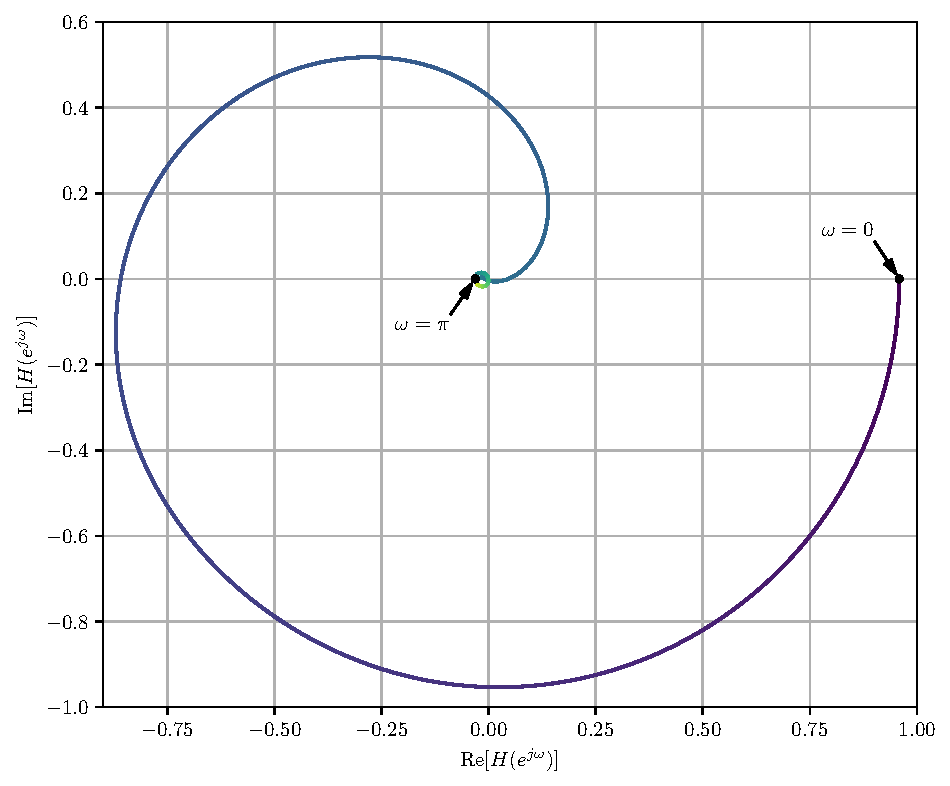
\includegraphics[width=0.95\textwidth]{figuras/transform_analysis_phase_unwrap_z_plane.pdf}
 \caption{\label{fig:transform_analysis_phase_unwrap_z_plane} Respuesta en frecuencia de un filtro FIR pasabajos en el plano complejo.}
 \end{center}
\end{figure}
El sistema de la figura corresponde a un filtro pasabajos, ya que tiene ganancia cercana a la unidad en \(\omega=0\) y ganancia cercana a cero en \(\omega=\pi\). Sin embargo, el valor principal de la fase en función de la frecuencia exhibe discontinuidades de \(2\pi\) radianes. Esto se ilustra en la figura \ref{fig:transform_analysis_phase_unwrap}, donde se muestra el valor principal de la fase \(\ARG[H(e^{j\omega})]\) del filtro pasabajos en el rango de frecuencias \(0\leq\omega\leq\pi\). Es común referirse a \(\ARG[H(e^{j\omega})]\) como la fase \emph{enrollada}. En la representación en magnitud y fase, suele ser útil \emph{desenrollar} la fase para obtener una función de fase continua con \(\omega\). Esto se logra sumando a la fase enrollada el múltiplo entero de \(2\pi\) apropiado \(r(\omega)\), como se muestra en la figura \ref{fig:transform_analysis_phase_unwrap}. La fase continua desenrollada se denotará como \(\arg[H(e^{j\omega})]\). Observar que es común que la fase, tanto enrollada como desenrollada, tenga saltos de \(\pi\) radianes. Esto ocurre en las frecuencias en donde la magnitud se anula, ya que en un entorno de esas frecuencias el número complejo \(H(e^{j\omega})\) puede pasar de un valor a su opuesto, lo que corresponde a un cambio de fase de \(\pi\) radianes.
\begin{figure}[!htb]
 \begin{center}
 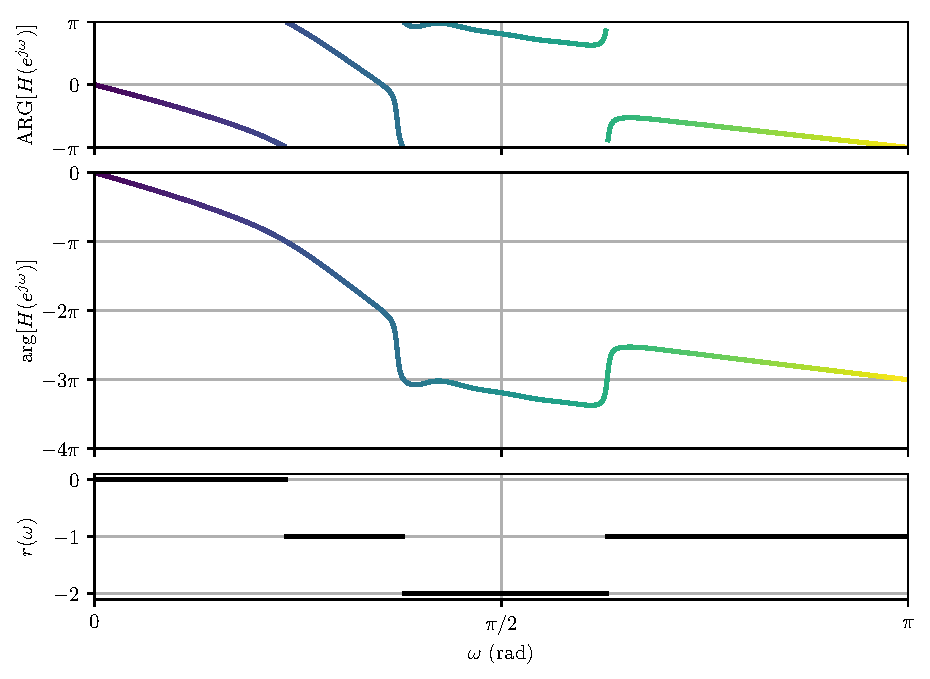
\includegraphics[width=0.95\textwidth]{figuras/transform_analysis_phase_unwrap.pdf}
 \caption{\label{fig:transform_analysis_phase_unwrap} Desenrollamiento del valor principal de la fase mediante la suma del múltiplo entero \(r(\omega)\) de \(2\pi\) apropiado. El color de las líneas de la respuesta en fase para cada frecuencia corresponde al mismo color en la misma frecuencia que la línea de \(H(e^{j\omega})\) en la figura \ref{fig:transform_analysis_phase_unwrap_z_plane}. }
 \end{center}
\end{figure}

Otra representación particularmente útil de la fase es el retardo de grupo \(\tau(\omega)\), definido como
\begin{equation}\label{eq:transform_analysis_group_delay_definition}
 \tau(\omega)=\grd[H(e^{j\omega})]=-\frac{d}{d\omega}\{\arg[H(e^{j\omega})]\}. 
\end{equation}
Para entender el efecto de la fase y específicamente del retardo de grupo, se considera primero el sistema retardo ideal. La respuesta al impulso es 
\[
 h_\textrm{id}[n]=\delta[n-n_d],
\]
y la respuesta en frecuencia es
\[
 H_\textrm{id}(e^{j\omega})=e^{-j\omega n_d},
\]
o
\begin{align*}
 |H_{id}(e^{j\omega})|&=1,\\
 \angle H_\textrm{id}(e^{j\omega})&=-\omega n_d,
 \qquad\qquad|\omega|<\pi,
\end{align*}
donde se asume periodicidad de \(2\pi\) en \(\omega\). Observar que el retardo temporal (o adelanto temporal si \(n_d<0\)) está asociado a una fase que varía linealmente con la frecuencia. En muchas aplicaciones, la distorsión de retardo se considera una forma moderada de distorsión de fase, ya que su efecto es solo desplazar a la señal en el tiempo.

El retardo de grupo definido por la ecuación \ref{eq:transform_analysis_group_delay_definition}, provee una medida apropiada de la linealidad de la fase. Específicamente, considérese la salida de un sistema con repuesta en frecuencia \(H(e^{j\omega})\) correspondiente a una entrada de banda angosta de la forma \(x[n]=s[n]\cos(\omega_0n)\). Como se asume que \(X(e^{j\omega})\) es únicamente no nula en torno a \(\omega=\omega_0\), el efecto de la fase del sistema en la banda de la señal puede aproximarse de forma lineal en torno a \(\omega=\omega_0\) como
\[
 \arg[H(e^{j\omega})]\approx-\phi_0-\omega n_d,
\]
donde \(n_d\) es el retardo de grupo. En el siguiente ejemplo se muestra que con esta aproximación, la respuesta \(y[n]\) a \(x[n]=s[n]\cos(\omega_0n)\) es aproximadamente \(y[n]=|H(e^{j\omega})|s[n-n_0]\cos(\omega_0n-\phi_0-\omega_0n_d)\). En consecuencia, el retardo temporal de la envolvente \(s[n]\) de la señal de banda angosta \(x[n]\) con transformada de Fourier centrada en \(\omega_0\) está dado por el retardo de grupo del sistema en \(\omega_0\). En general, una señal de banda ancha se puede considerar como la superposición de señales de banda angosta centradas en distinta frecuencia. Si el retardo de grupo es constante con la frecuencia, cada componente de banda angosta sufrirá una retardo idéntico. Si el retardo de grupo no es constante, el retardo de cada componente da banda angosta será distinto, resultando en la dispersión temporal de la energía de la señal. Por lo tanto, una respuesta en fase no lineal, o equivalentemente, un retardo de grupo no constante produce dispersión temporal.

\paragraph{Ejemplo: estudio del efecto del retardo de grupo en una señal de banda angosta} Este ejemplo es el problema 5.63 de \cite{oppenheim2009discrete}. Sea un sistema con respuesta en frecuencia \(H(e^{j\omega})\) con entrada de la forma \(x[n]=s[n]\cos(\omega_0n)\), donde \(s[n]\) es una señal banda base de banda relativamente angosta, es decir, \(S(e^{j\omega})=0\) en \(|\omega|>\Delta\), con \(\Delta\ll\omega_0\), de forma de que \(X(e^{j\omega})\) es de banda angosta en torno a \(\omega=\pm\omega_0\). Del teorema del desplazamiento en frecuencia (ver la sección \ref{sec:fourier_transform_theorems}) de la transformada de Fourier, la transformada de \(x[n]\) en términos de la transformada de \(s[n]\) es
\[
 X(e^{j\omega})=\frac{1}{2}\left[S(e^{j(\omega-\omega_0)})+S(e^{j(\omega+\omega_0)})\right].
\]
\begin{figure}[!htb]
 \begin{center}
 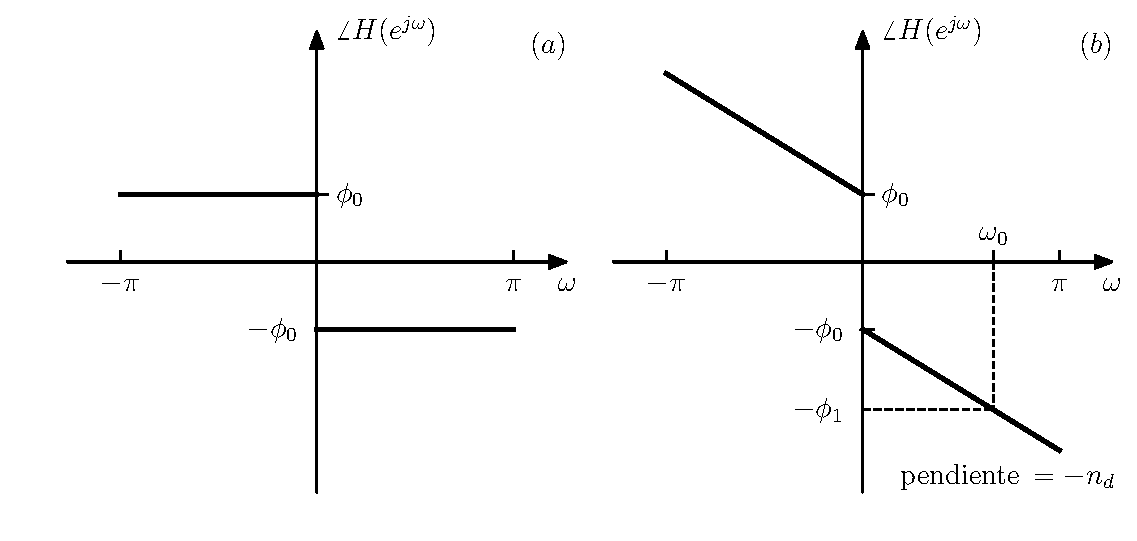
\includegraphics[width=0.87\textwidth]{figuras/problem_5_63_phase_responses.pdf}
 \caption{\label{fig:problem_5_63_phase_responses} Respuesta en fase del sistema de los casos \((a)\) y \((b)\) del ejemplo.}
 \end{center}
\end{figure}
Se asume que la respuesta en magnitud del sistema es \(|H(e^{j\omega})|=1\), y para la respuesta en fase se consideran los siguientes casos:
\begin{enumerate}
 \item[\((a)\)] \(\angle H(e^{j\omega})\) es como se muestra en la gráfica \((a)\) de la figura \ref{fig:problem_5_63_phase_responses}. La transformada de Fourier de la salida del sistema es
 \begin{align*}
  Y(e^{j\omega})&=H(e^{j\omega})X(e^{j\omega})\\
   &=\frac{1}{2}\left[S(e^{j(\omega-\omega_0)})e^{-j\phi_0}+S(e^{j(\omega+\omega_0)})e^{j\phi_0}\right],
 \end{align*}
donde se consideró que como \(S(e^{j\omega})\) es de banda angosta, los componentes \(S(e^{j(\omega-\omega_0)})\) y \(S(e^{j(\omega+\omega_0)})\) no se interfieren, y el primero solo es no nulo en las frecuencias positivas en torno a \(\omega_0\) y el segundo solo es no nulo en las frecuencias negativas en torno a \(-\omega_0\). Luego, considerando nuevamente el teorema del desplazamiento en frecuencia y la linealidad de la transformada de Fourier, la salida en el dominio del tiempo es
\begin{align*}
 y[n]&=\frac{1}{2}\left(s[n]e^{j\omega_0n}e^{-j\phi_0}+s[n]e^{-j\omega_0n}e^{j\phi_0}\right)\\
  &=s[n]\frac{e^{j(\omega_0n-\phi_0)}+e^{-j(\omega_0n-\phi_0)}}{2},
\end{align*}
resultando en que 
\[
 y[n]=s[n]\cos(\omega_0n-\phi_0).
\]
 \item[\((b)\)] Ahora, \(\angle H(e^{j\omega})\) es como se muestra en la gráfica \((b)\) de la figura \ref{fig:problem_5_63_phase_responses}, es decir,
\[
 \angle H(e^{j\omega})=
 \left\{ 
 \begin{array}{ll}
  \phi_0-\omega n_d & -\pi<\omega<0\\
  -\phi_0-\omega n_d & 0<\omega<\pi
 \end{array}
 \right.
\]
con periodicidad \(2\pi\). La transformada de Fourier de la salida es
\begin{align}
  Y(e^{j\omega})&=H(e^{j\omega})X(e^{j\omega})\nonumber\\
   &=\frac{1}{2}\left[S(e^{j(\omega-\omega_0)})e^{j(-\phi_0-\omega n_d)}+S(e^{j(\omega+\omega_0)})e^{j(\phi_0-\omega n_d)}\right]\nonumber\\
    &=\frac{1}{2}\left[S(e^{j(\omega-\omega_0)})e^{-j\omega n_d}e^{-j\phi_0}+S(e^{j(\omega+\omega_0)})e^{-j\omega n_d}e^{j\phi_0}\right]\label{eq:transform_analysis_exercise_5_63_b_output_dtft}
\end{align}
donde se consideró el mismo argumento que antes. Luego, teniendo en cuenta que 
\[
 s[n]e^{j\omega_0n}\;\overset{\mathcal{F}}{\longleftrightarrow}\;S(e^j(\omega-\omega_0))
 \qquad\qquad\textrm{y}\qquad\qquad
 \delta[n-n_d]\;\overset{\mathcal{F}}{\longleftrightarrow}\;e^{-j\omega n_d},
\]
donde se asumió que \(n_d\) es un número entero, se cumple que 
\[
 s[n]e^{j\omega_0n}*\delta[n-n_d]\;\overset{\mathcal{F}}{\longleftrightarrow}\;S(e^{j(\omega-\omega_0)})e^{-j\omega n_d},
\]
es decir,
\[
 s[n-n_d]e^{j\omega_0(n-n_d)}\;\overset{\mathcal{F}}{\longleftrightarrow}\;S(e^{j(\omega-\omega_0)})e^{-j\omega n_d}.
\]
Realizando el mismo razonamiento para el segundo sumando de la ecuación \ref{eq:transform_analysis_exercise_5_63_b_output_dtft}, se cumple que 
\[
 s[n-n_d]e^{-j\omega_0(n-n_d)}\;\overset{\mathcal{F}}{\longleftrightarrow}\;S(e^{j(\omega+\omega_0)})e^{-j\omega n_d},
\]
por lo que que la salida en el dominio del tiempo es 
\begin{align*}
 y[n]&=\frac{1}{2}\left\{s[n-n_d]e^{j\omega_0(n-n_d)}e^{-j\phi_0}+s[n-n_d]e^{-j\omega_0(n-n_d)}e^{j\phi_0}\right\}\\
  &=s[n-n_d]\frac{e^{j[\omega_0(n-n_d)-\phi_0]}+e^{-j[\omega_0(n-n_d)-\phi_0]}}{2}\\
  &=s[n-n_d]\cos[\omega_0(n-n_d)-\phi_0],
\end{align*}
o
\begin{equation}\label{eq:transform_analysis_exercise_5_63_b_output}
 y[n]=s[n-n_d]\cos[\omega_0n-\phi_0-\omega_0n_d]. 
\end{equation}
Si la fase en \(\omega_0\) es \(\phi_1\), como se muestra en la figura \ref{fig:problem_5_63_phase_responses}, es decir,
\[
 -\phi_0-\omega_0n_d=-\phi_1,
\]
resulta en que
\[
 y[n]=s[n-n_d]\cos[\omega_0n-\phi_1].
\]
 \item[\((c)\)] Ahora la fase es una función arbitraria con retardo de grupo y retardo de fase en \(\omega_0\) los números enteros \(\tau_\textrm{gr}(\omega_0)\) y \(\tau_\textrm{ph}(\omega_0)\) respectivamente (ver las ecuaciones \ref{eq:transform_analysis_group_delay_definition} y \ref{eq:seq_and_sys_phase_delay_definition}). Como la transformada de Fourier de la entrada es
 \[
  X(e^{j\omega})=\frac{1}{2}\left[S(e^{j(\omega-\omega_0)})+S(e^{j(\omega+\omega_0)})\right],
 \]
 y \(S(e^{j(\omega-\omega_0)})\) es de banda angosta en torno a \(\omega_0\), la respuesta en fase del sistema se puede aproximar por una recta en al ancho de banda de la señal, como se muestra en la figura \ref{fig:transform_analysis_group_delay_input_and_linealization}. Realizando un desarrollo de Taylor de primer orden de la función de fase en torno al punto \(\omega=\omega_0\), se cumple que
 \[
  \arg{H(e^{j\omega})}\approx\arg H(e^{j\omega_0})+\frac{d}{d\omega}\left[\arg H(e^{j\omega})\right]\bigg|_{\omega=\omega_0}(\omega-\omega_0)
 \]
 en \(\omega\approx\omega_0\). 
 \begin{figure}[!htb]
 \begin{center}
 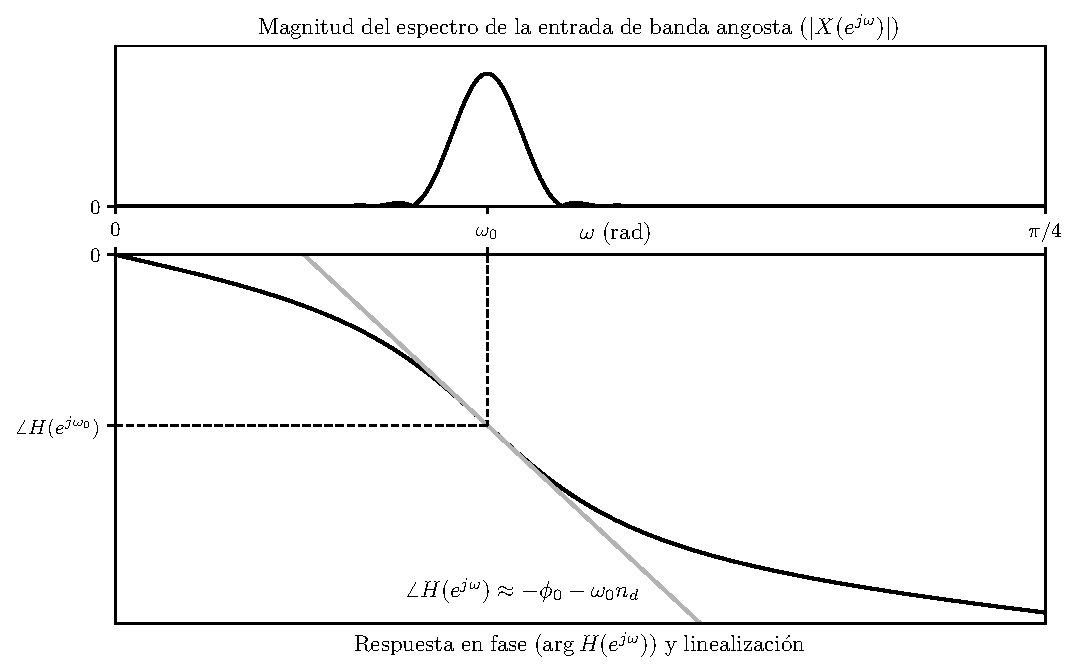
\includegraphics[width=\textwidth]{figuras/transform_analysis_group_delay_input_and_linealization.pdf}
 \caption{\label{fig:transform_analysis_group_delay_input_and_linealization} Magnitud de la entrada \(|X(e^{j\omega})|\) y respuesta en fase del sistema \(\arg H(e^{j\omega})\). Como la entrada es de banda angosta, la fase se puede aproximar como una función lineal en la banda de la entrada.}
 \end{center}
\end{figure}
 Como por definición,
 \[
  \tau_\textrm{gr}(\omega_0)=-\frac{d}{d\omega}\left[\arg H(e^{j\omega})\right]\bigg|_{\omega=\omega_0}
  \qquad\qquad\textrm{y}\qquad\qquad
  \tau_\textrm{gr}(\omega_0)=-\frac{\arg H(e^{j\omega_0})}{\omega_0},
 \]
 la aproximación lineal de la fase puede expresarse en términos del retardo de grupo y el retardo de fase como
 \begin{align*}
  \arg{H(e^{j\omega})}&\approx-\tau_\textrm{ph}(\omega_0)\omega_0-\tau_\textrm{gr}(\omega_0)(\omega-\omega_0)\\
   &\approx-\omega_0[\tau_\textrm{ph}(\omega_0)-\tau_\textrm{gr}(\omega_0)]-\omega\tau_\textrm{gr}(\omega_0).
 \end{align*}
 Por lo tanto, los parámetros \(\phi_0\) y \(n_d\) correspondientes al corte por cero y a la pendiente de la linealización de la fase en la parte \((b)\) son respectivamente
 \[
  \phi_0=\omega_0[\tau_\textrm{ph}(\omega_0)-\tau_\textrm{gr}(\omega_0)]
  \qquad\qquad\textrm{y}\qquad\qquad
  n_d=\tau_\textrm{gr}(\omega_0).
 \]
 Sustituyendo estos parámetros en la ecuación \ref{eq:transform_analysis_exercise_5_63_b_output}, la salida queda
 \[
  y[n]\approx s[n-\tau_\textrm{gr}(\omega_0)]\cos\left\{\omega_0n-\omega_0[\tau_\textrm{ph}(\omega_0)-\tau_\textrm{gr}(\omega_0)]-\omega_0\tau_\textrm{gr}(\omega_0)\right\}
 \]
 resultando en 
 \begin{equation}\label{eq:transform_analysis_exercise_5_63_c_output}
  y[n]\approx s[n-\tau_\textrm{gr}(\omega_0)]\cos\left\{\omega_0[n-\tau_\textrm{ph}(\omega_0)]\right\}.  
 \end{equation}
 Esta ecuación indica que para una señal de banda angosta \(x[n]\), el efecto de la fase \(\angle H(e^{j\omega})\) del filtro es aplicar un retardo \(\tau_\textrm{gr}(\omega_0)\) a la envolvente \(s[n]\) y un retardo \(\tau_\textrm{ph}(\omega_0)\) a la portadora \(\cos\omega_0n\).
 
 Observar que la ecuación \ref{eq:transform_analysis_exercise_5_63_c_output} es válida solo si \(n_d=\tau_\textrm{gr}(\omega_0)\) es un número entero, ya que la transformada inversa de \(e^{-j\omega n_d}\) es \(\delta[n-n_d]\) si \(n_d\) es un número entero, hecho que se empleó para obtener la ecuación \ref{eq:transform_analysis_exercise_5_63_b_output}. Si \(n_d=\Delta\) no es entero, aplicando la transformada Fourier inversa, se puede mostrar que 
 \[
  \frac{\sen\pi(n-\Delta)}{\pi(n-\Delta)}\;\overset{\mathcal{F}}{\longleftrightarrow}\;e^{-j\omega\Delta}.
 \]
 De todas formas, si \(\tau_\textrm{gr}(\omega_0)\) o \(\tau_\textrm{ph}(\omega_0)\) o ambos no son enteros, el efecto sobre la envolvente y la portadora es el mismo, con la interpretación de un retardo no entero explicada en la sección 4.5 de \cite{oppenheim2009discrete}, que consiste en convertir la señal de tiempo discreto a tiempo continuo (ver la sección 4.3 de \cite{oppenheim2009discrete}), aplicar un retardo arbitrario en tiempo continuo y muestrear la señal resultante para obtener una señal en tiempo discreto.
 
Como ilustración del efecto del retardo de fase y el retardo de grupo, considérese el sistema con repuesta en fase que se muestra en la figura \ref{fig:transform_analysis_group_delay_phase_and_group_delay}. 
\begin{figure}[!htb]
 \begin{center}
 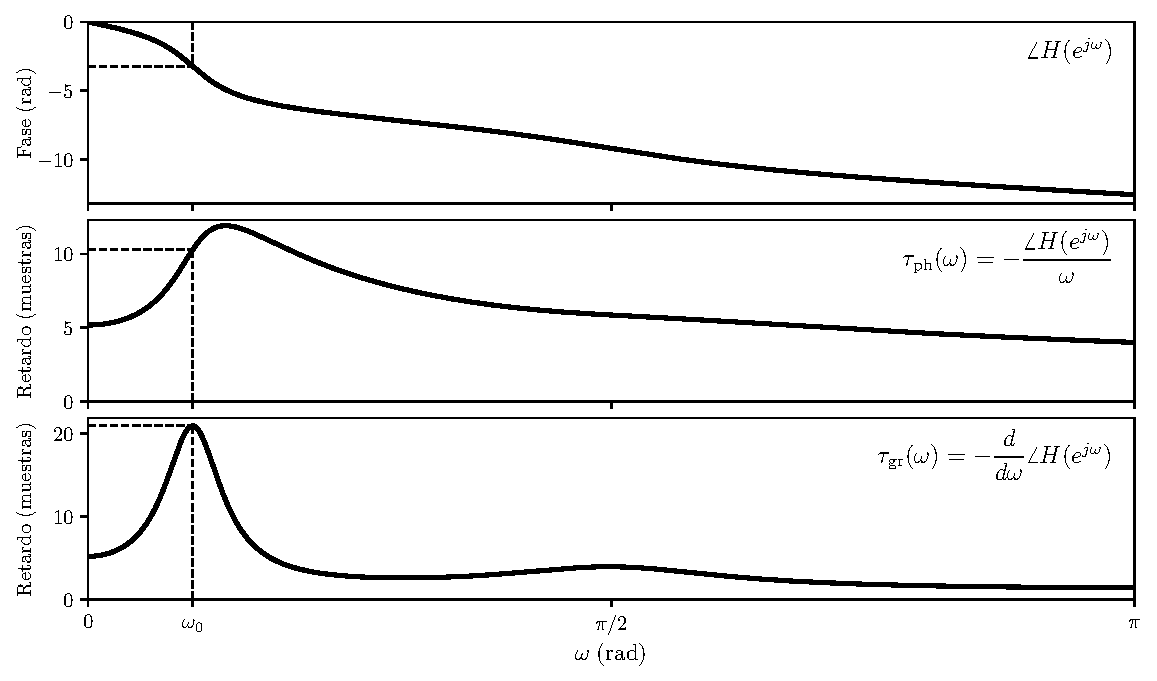
\includegraphics[width=\textwidth]{figuras/transform_analysis_group_delay_phase_and_group_delay.pdf}
 \caption{\label{fig:transform_analysis_group_delay_phase_and_group_delay} Respuesta en fase, retardo de fase y retardo de grupo. En la frecuencia \(\omega_0\) el retardo de fase es aproximadamente 10.3 muestras y el retardo de grupo es aproximadamente 20.9 muestras.}
 \end{center}
\end{figure}
En la figura se muestra además el correspondiente retardo de grupo \(\tau_\textrm{gr}(\omega)\) y retardo de fase \(\tau_\textrm{ph}(\omega)\). Sea la entrada de banda angosta \(x[n]=s[n]\cos\omega_0n\) con espectro como el que se muestra en la figura \ref{fig:transform_analysis_group_delay_input_and_linealization}. La respuesta en magnitud del sistema es la unidad en la frecuencia \(\omega_0\) de la portadora. Como se observa en la figura \ref{fig:transform_analysis_group_delay_phase_and_group_delay}, en la frecuencia \(\omega_0\), el retardo de fase es \(\tau_\textrm{ph}(\omega_0)\approx10.3\) muestras y el retardo de grupo es \(\tau_\textrm{gr}(\omega_0)\approx20.9\) muestras. En la figura \ref{fig:transform_analysis_group_delay_input_output} se muestra la entrada y la correspondiente salida. Se observa que el retardo de la portadora, por ejemplo midiendo la distancia entre un máximo de la sinusoide de entrada y el correspondiente máximo de la sinusoide de salida, es el retardo de fase \(\tau_\textrm{ph}(\omega_0)\), mientras que el retardo de la envolvente, que se puede obtener midiendo la distancia entre los máximos de la envolvente de la entrada y de la salida, es el retardo de grupo \(\tau_\textrm{gr}(\omega_0)\), acorde con el resultado de la ecuación \ref{eq:transform_analysis_exercise_5_63_c_output}. 
\begin{figure}[!htb]
 \begin{center}
 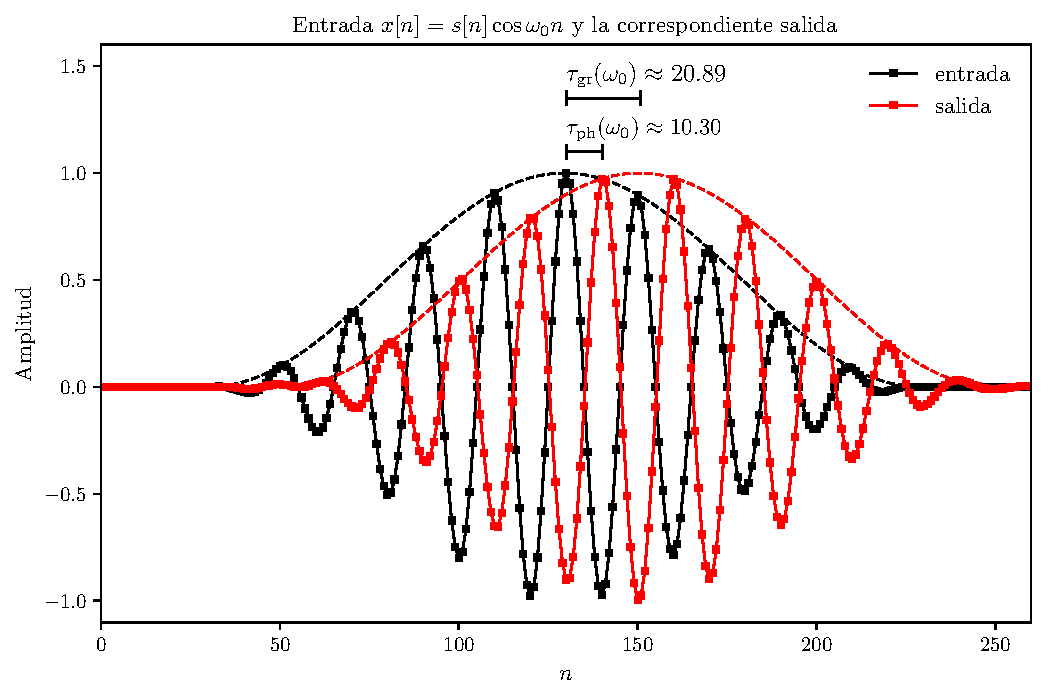
\includegraphics[width=\textwidth]{figuras/transform_analysis_group_delay_input_output.pdf}
 \caption{\label{fig:transform_analysis_group_delay_input_output} Señal de entrada y señal de salida. El retardo de la portadora es \(\tau_\textrm{ph}(\omega_0)\approx10.3\) muestras y el retardo de la envolvente es \(\tau_\textrm{gr}(\omega_0)\approx20.9\) muestras.}
 \end{center}
\end{figure} 
\end{enumerate}

\paragraph{Ejemplo: otra ilustración del efecto del retardo de grupo en una señal de banda angosta} Este ejemplo es una variación del ejemplo de la sección 5.1.2 de \cite{oppenheim2009discrete}. Se considera ahora el sistema con función de transferencia
\begin{equation}\label{eq:transform_analysis_example_5_1_2_system_function}
 H(z)=\prod_{k=1}^4\left[\frac{(c^*_k-z^{-1})(c_k-z^{-1})}{(1-c_kz^{-1})(1-c^*_kz^{-1})}\right]^2, 
\end{equation}
donde \(c_k=0.95e^{j(0.15\pi+0.02\pi k)}\) para \(k=1,\,2,\,3,\,4\). Este sistema tiene polos dobles en \(z=c_k=0.95e^{j(0.15\pi+0.02\pi k)}\) y en \(z=c^*_k=0.95e^{-j(0.15\pi+0.02\pi k)}\) y ceros dobles en \(z=1/c_k=0.95e^{-j(0.15\pi+0.02\pi k)}\) y en \(z=1/c^*_k=0.95e^{j(0.15\pi+0.02\pi k)}\). Como se verá mas adelante en la sección \ref{}, \(H(z)\) es un sistema pasa todo, es decir, \(|H(e^{j\omega})|=1\) para todo \(\omega\). Como se ilustrará, este sistema introduce un retardo de grupo grande sobre una banda angosta de frecuencias.
 \begin{figure}[!htb]
  \begin{minipage}[c]{0.53\textwidth}
    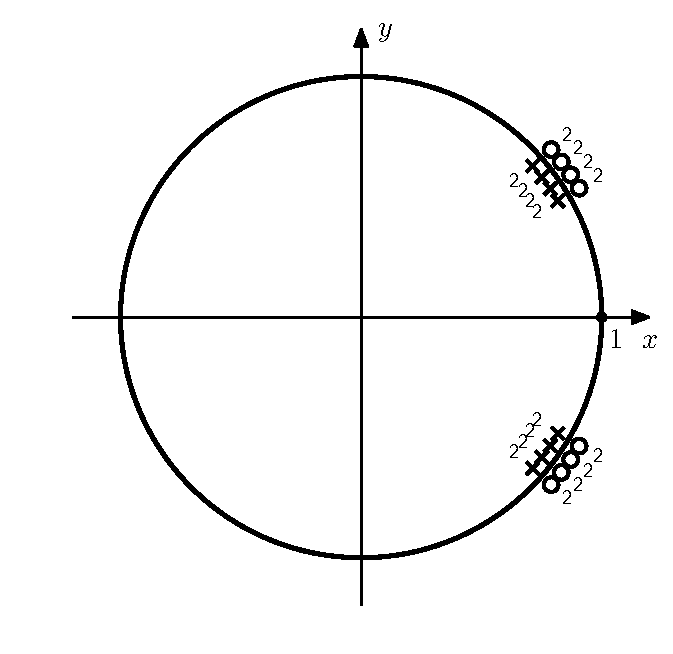
\includegraphics[width=\textwidth]{figuras/transform_analysis_example_5_1_2_group_delay_poles_zeros_plot.pdf}
  \end{minipage}\hfill
  \begin{minipage}[c]{0.38\textwidth}
    \caption{
     Diagrama de polos y ceros del sistema \(H(z)\).
    }\label{fig:transform_analysis_example_5_1_2_group_delay_poles_zeros_plot}
  \end{minipage}
\end{figure}
\\
En la figura \ref{fig:transform_analysis_example_5_1_2_group_delay_frequency_response} se muestra la respuesta en frecuencia del sistema. Como ya se mencionó, se observa que la respuesta en magnitud es unitaria en todas las frecuencias, como corresponde a un sistema pasa todo. Además, el valor principal de la fase tiene exhibe múltiples discontinuidades de tamaño \(2\pi\) en torno a la frecuencia \(\omega=0.2\pi\) radianes. Esta frecuencia corresponde la fase central del grupo de polos y ceros del sistema, cuyas fases son \(\pm0.17\pi\), \(\pm0.19\pi\), \(\pm0.21\pi\) y \(\pm0.23\pi\) radianes, tanto para los ceros como para los polos.
\begin{figure}[!htb]
 \begin{center}
 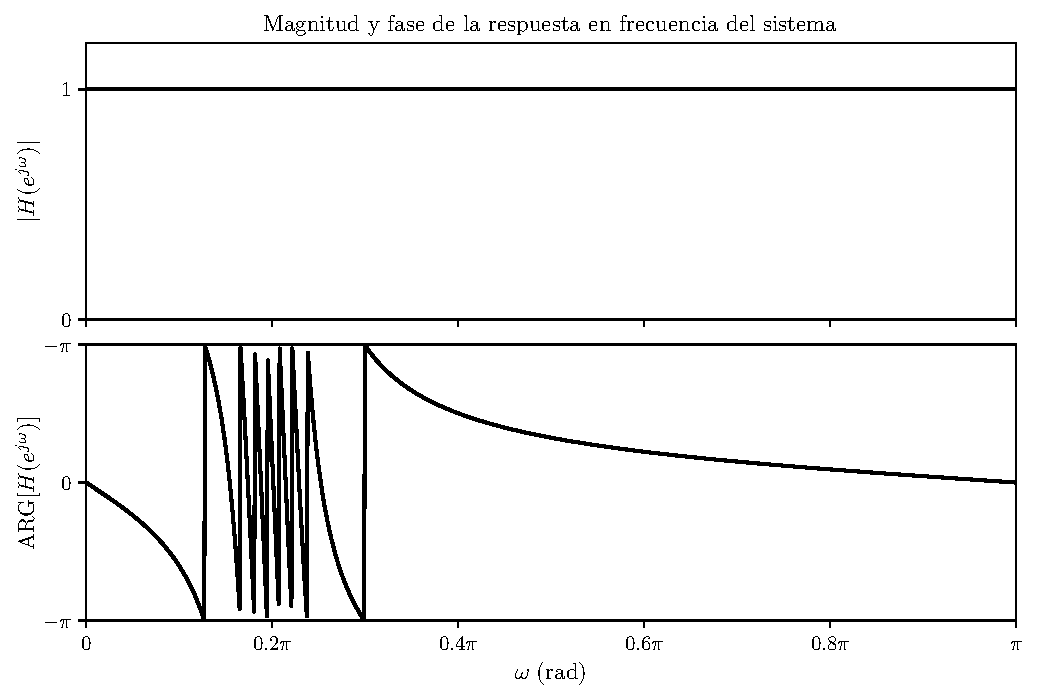
\includegraphics[width=\textwidth]{figuras/transform_analysis_example_5_1_2_group_delay_frequency_response.pdf}
 \caption{\label{fig:transform_analysis_example_5_1_2_group_delay_frequency_response} Respuesta en magnitud y respuesta en fase del sistema \(H(z)\).}
 \end{center}
\end{figure} 
\\
En la figura \ref{fig:transform_analysis_example_5_1_2_group_delay} se muestra la respuesta en fase desenrollada y el retardo de grupo del sistema. Se observa que, como la fase es monótonamente decreciente, el retardo de grupo es positivo. Además se ve que el retardo de grupo tiene un pico positivo grande en una banda de frecuencia en torno a \(0.2\pi\) radianes,  que corresponde a la ubicación angular del grupo de polos y ceros mostrados en la figura \ref{fig:transform_analysis_example_5_1_2_group_delay_poles_zeros_plot}.
\begin{figure}[!htb]
 \begin{center}
 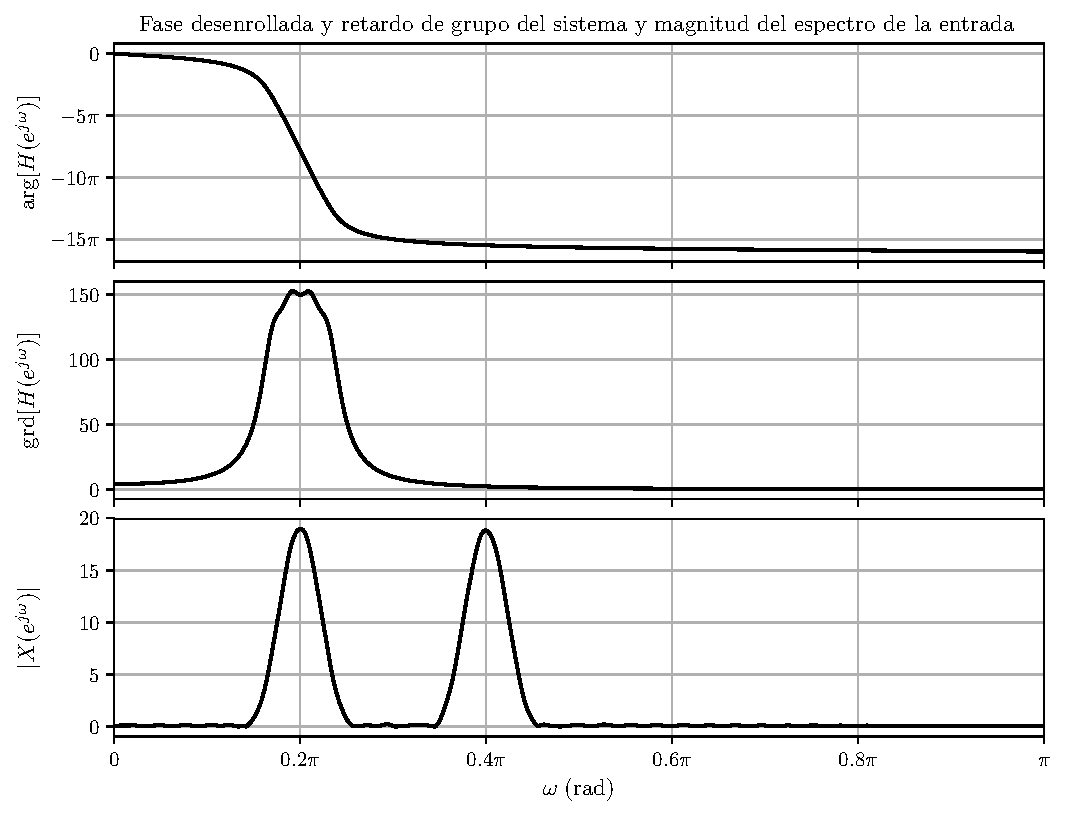
\includegraphics[width=\textwidth]{figuras/transform_analysis_example_5_1_2_group_delay.pdf}
 \caption{\label{fig:transform_analysis_example_5_1_2_group_delay} Fase desenrollada y retardo de grupo del sistema. También se muestra la magnitud del espectro de la señal de entrada. Se observa que la sinusoide de entrada de frecuencia \(\omega_1=0.2\pi\) se ve afectada por un retardo de grupo de alrededor de 150 muestras mientras que la sinusoide de frecuencia \(\omega_1=0.4\pi\) se ve afectada por un retardo de grupo pequeño (2.5 muestras aproximadamente).}
 \end{center}
\end{figure} 
\\
Como entrada al sistema se considera una señal que consiste en dos pulsos de banda angosta separados en el tiempo. Los pulsos son
\[
 x_1[n]=w[n]\cos(0.2\pi n)
 \qquad\qquad\textrm{y}\qquad\qquad
 x_2[n]=w[n]\cos(0.4\pi n-\pi/2),
\]
donde la envolvente \(w[n]\) de cada sinusoide es un ventana de Hamming de 71 muestras,
\[
 w[n]=\left\{ 
 \begin{array}{ll}
  0.54-0.46\cos(2\pi n/M) & 0\leq n\leq M\\
  0 &\textrm{en otro caso},
 \end{array}
 \right.
\]
donde \(M=70\). La secuencia completa de entrada es
\[
 x[n]=x_1[n]+x_2[n-M-1],
\]
es decir, la sinusoide de menor frecuencia viene primero seguida de la sinusoide de mayor frecuencia. En la figura \ref{fig:transform_analysis_example_5_1_2_group_delay} se muestra la magnitud del espectro de la señal de entrada. Como es de esperar por el teorema de modulación (ver la sección \ref{sec:fourier_transform_theorems}), la señal tiene alta energía en torno a las frecuencias de las sinusoides \(\omega_1=0.2\pi\) y \(\omega_2=0.4\pi\). La forma de los pulsos de alta energía son la transformada de Fourier de la ventana temporal.
\\
Cuando se emplea \(x[n]\) como entrada al sistema \(H(z)\), cada banda de frecuencia asociado a cada una de las sinusoides será afectada por la repuesta en magnitud y el retardo de grupo del sistema en cada banda de frecuencia. Como el sistema es un filtro pasa todo, no afecta la magnitud de las sinusoides. Examinando el retardo de grupo en la figura \ref{fig:transform_analysis_example_5_1_2_group_delay} se ve que el retardo de grupo en torno a la frecuencia \(\omega=\omega_1=0.2\pi\) es significativamente mayor que el correspondiente a la frecuencia \(\omega=\omega_2=0.4\pi\), y en consecuencia, la sinusoide de menor frecuencia experimentará un mayor retardo.
\\
La entrada \(x[n]\) y la correspondiente salida \(y[n]\) son mostradas en la figura \ref{fig:transform_analysis_example_5_1_2_group_delay_input_output}. El pulso sinusoidal de frecuencia \(\omega_1=0.2\pi\) es retardado unas 150 muestras, mientras que el pulso sinusoidal de frecuencia \(\omega_2=0.4\pi\) es retardado unas 2 muestras. De hecho, como la sinusoide de baja frecuencia es retardada unas 147 muestras mas que la sinusoide de alta frecuencia y el largo de los pulsos sinusoidales es de 71 muestras, los pulsos son intercambiados de orden temporal en la salida, como se ve en la figura.
\begin{figure}[!htb]
 \begin{center}
 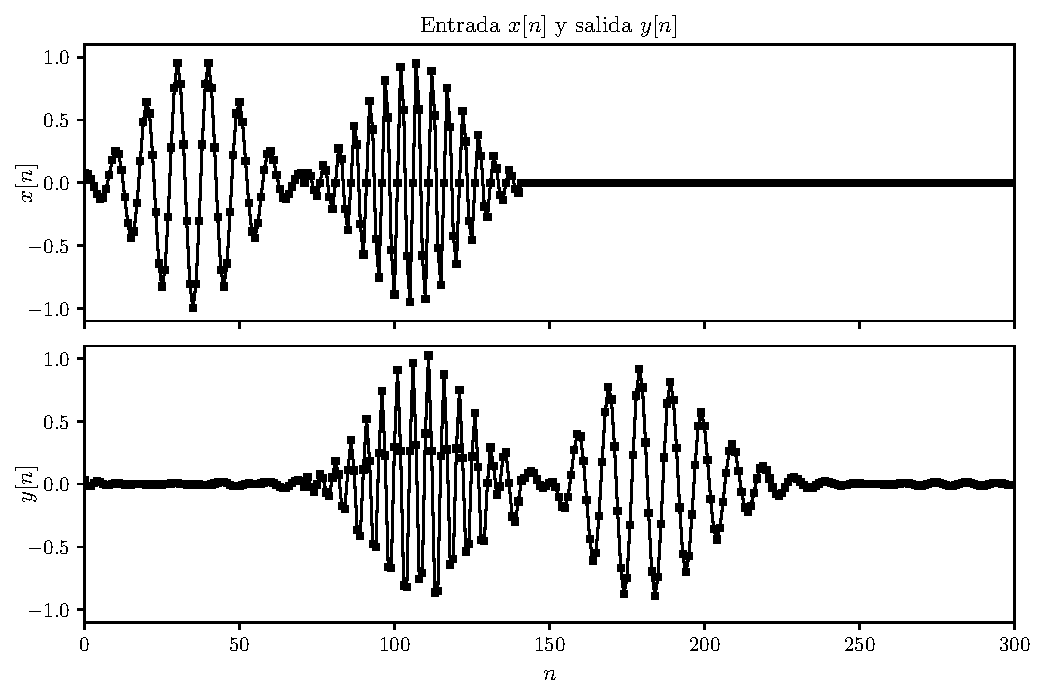
\includegraphics[width=\textwidth]{figuras/transform_analysis_example_5_1_2_group_delay_input_output.pdf}
 \caption{\label{fig:transform_analysis_example_5_1_2_group_delay_input_output} Entrada y salida del sistema. Debido al alto retardo de grupo que afecta al pulso sinusoidal de menor frecuencia, el orden de ambos pulsos es intercambiado en la salida.}
 \end{center}
\end{figure}
\\
Finalmente, se realizan algunas consideraciones sobre la implementación del filtro en el lenguaje de programación Python. Cuando la función de transferencia es racional, como es el caso de \(H(z)\) dado por la ecuación \ref{eq:transform_analysis_example_5_1_2_system_function} del presente ejemplo, el sistema en el dominio del tiempo está dado por una ecuación en diferencias de la forma \ref{eq:seq_and_sys_difference_equation_general}, y hay una relación directa entre los coeficientes de la ecuación en diferencias y los coeficientes de los polinomios del numerador y denominador de la función de transferencia. Concretamente, la función de transferencia del sistema dado por \ref{eq:seq_and_sys_difference_equation_general} es
\begin{equation}\label{eq:transform_analysis_system_function_ba}
 H(z)=\frac{Y(z)}{X(z)}=\frac{\displaystyle\sum_{k=0}^Mb_kz^{-k}}{\displaystyle\sum_{k=0}^Na_kz^{-k}}. 
\end{equation}
En el caso de este ejemplo, la función del sistema está dada por los polos y ceros del sistema, es decir, por las raíces de los polinomios del numerador y denominador. Una forma de obtener los coeficientes de los polinomios a partir de las raíces de los polinomios es mediante la función \texttt{zpk2tf} de la biblioteca SciPy \cite{2020SciPy-NMeth}. Dicha función asume que la función de transferencia racional está factorizada como
\begin{equation}\label{eq:transform_analysis_system_function_zpk}
 H(z)=k\frac{\displaystyle\prod_{k=1}^M(z-c_k)}{\displaystyle\prod_{k=1}^N(z-d_k)} 
\end{equation}
y recibe como parámetros los vectores \(\z\) y \(\mathbf{p}\) conteniendo respectivamente los ceros \(c_k\) y los polos \(d_k\), además del valor \(k\) de la ganancia de la función del sistema \ref{eq:transform_analysis_system_function_zpk} y calcula y devuelve los vectores \(\mathbf{b}\) y \(\mathbf{a}\) conteniendo respectivamente los coeficientes \(b_k\) y \(a_k\) de la representación \ref{eq:transform_analysis_system_function_ba}, que como se mencionó, son los mismos que los de la ecuación en diferencias \ref{eq:seq_and_sys_difference_equation_general}. Para expresar la función del sistema \ref{eq:transform_analysis_example_5_1_2_system_function} de este ejemplo de la forma \ref{eq:transform_analysis_system_function_zpk} para emplear la función \texttt{zpk2tf}, se observa que cada término pasa todo en \ref{eq:transform_analysis_example_5_1_2_system_function}, puede expresarse como
\[
 \frac{c^*_k-z^{-1}}{1-c_kz^{-1}}=\frac{zc^*_k-1}{z-c_k}=c^*_k\frac{z-1/c^*_k}{z-c_k},
\]
y por lo tanto, dicha ecuación puede expresarse como
\begin{align*}
 H(z)&=\prod_{k=1}^4\left[c_kc^*_k\frac{(z-1/c^*_k)(z-1/c_k)}{(z-c_k)(z-c^*_k)}\right]^2\\
  &=\prod_{k=1}^4\left[|c_k|^2\frac{(z-1/c^*_k)(z-1/c_k)}{(z-c_k)(z-c^*_k)}\right]^2\\
  &=\prod_{k=1}^4|c_k|^4\prod_{k=1}^4\left[\frac{(z-1/c^*_k)(z-1/c_k)}{(z-c_k)(z-c^*_k)}\right]^2. 
\end{align*}
De esta forma,
\[
 k=\prod_{k=1}^4|c_k|^4,
\]
el vector \(\z\) de ceros contiene los valores \(1/c_k\) y \(1/c^*_k\) duplicados, ya que son ceros dobles debido a la elevación al cuadrado, y el vector \(\mathbf{p}\) de polos contiene los valores \(c_k\) y \(c^*_k\), también duplicados por la misma razón.
\begin{figure}
\begin{center}
\lstinputlisting{figuras/transform_analysis_filter_ba_coefs_from_zpk.py}
\caption{\label{fig:transform_analysis_filter_ba_coefs_from_zpk} Implementación en el lenguaje Python del cálculo de los coeficientes \(\mathbf{b}\) y \(\mathbf{a}\) a partir del conjunto de ceros \(\z\), polos \(\mathbf{p}\) y la ganancia \(k\) del filtro empleado en este ejemplo.}
\end{center}
\end{figure}
En la figura \ref{fig:transform_analysis_filter_ba_coefs_from_zpk} se incluye el código en el lenguaje Python para el cálculo de los coeficientes \(\mathbf{b}\) y \(\mathbf{a}\) a partir del conjunto de ceros \(\z\), polos \(\mathbf{p}\) y la ganancia \(k\) del filtro dado por la ecuación \ref{eq:transform_analysis_example_5_1_2_system_function}.

\section{Sistemas caracterizados por ecuaciones en diferencias lineales con coeficientes constantes}

Los filtros en el dominio del tiempo discreto son típicamente implementados mediante una ecuación en diferencias lineal con coeficientes constantes de la forma
\begin{equation}\label{eq:transform_analysis_difference_equation_general}
 \sum_{k=0}^Na_ky[n-k]=\sum_{k=0}^Mb_kx[n-k]. 
\end{equation}
En el capítulo \ref{} se discuten varias estructuras para la realización de estos sistemas y en el capítulo \ref{} se discuten varios procedimientos para la obtención de los parámetros de la ecuación en diferencias para aproximar una respuesta en frecuencia deseada. En esta sección se examinan las propiedades y características de los sistemas LTI representados por la ecuación \ref{eq:transform_analysis_difference_equation_general} con la ayuda de la transformada \(z\).

Aplicando la transformada \(z\) a ambos lados de la ecuación \ref{eq:transform_analysis_difference_equation_general} se obtiene que la función del sistema tiene la forma algebraica
\begin{equation}\label{eq:transform_analysis_difference_equation_system_function_ba}
 H(z)=\frac{Y(z)}{X(z)}=\frac{\displaystyle\sum_{k=0}^Mb_kz^{-k}}{\displaystyle\sum_{k=0}^Na_kz^{-k}}. 
\end{equation}
En ocasiones, es conveniente expresar la ecuación \ref{eq:transform_analysis_difference_equation_system_function_ba} en forma factorizada como
\begin{equation}\label{eq:transform_analysis_difference_equation_system_function_zp}
 H(z)=\left(\frac{b_0}{a_0}\right)\frac{\prod\limits_{k=1}^M(1-c_kz^{-1})}{\prod\limits_{k=1}^N(1-d_kz^{-1})}. 
\end{equation}
Cada uno de los factores \((1-c_kz^{-1})\) en el numerador contribuye con un cero en \(z=c_k\) y con un polo en \(z=0\) y cada uno de los factores \((1-d_kz^{-1})\) en el denominador contribuye con un cero en \(z=0\) y con un polo en \(z=d_k\). 

\subsection{Estabilidad y causalidad}

Para obtener la ecuación \ref{eq:transform_analysis_difference_equation_system_function_ba} a partir de la ecuación \ref{eq:transform_analysis_difference_equation_general} se asume que el sistema es lineal e invariante en el tiempo de forma de que se cumple la ecuación \ref{eq:transform_analysis_input_output_system_function_lti}, pero no se realizó ninguna hipótesis sobre estabilidad o causalidad. De forma correspondiente, si bien de la ecuación en diferencias puede obtenerse la función del sistema, no puede especificarse la región de convergencia. Específicamente, la ROC de \(H(z)\) no queda determinada en la deducción que conduce a la ecuación \ref{eq:transform_analysis_difference_equation_system_function_ba}, ya que lo único que se requiere para que se cumple dicha ecuación es que \(X(z)\) y \(Y(z)\) tengan ROCs que se solapen (para la existencia de \(H(z)\)). Esto es consistente con el hecho de que la ecuación en diferencias no especifica unívocamente la repuesta al impulso del sistema LTI, como se discutió en la sección \ref{sec:seq_and_sys_constant_coefficient_difference_equations}. Para el sistema de la ecuación \ref{eq:transform_analysis_difference_equation_system_function_ba} o de la ecuación \ref{eq:transform_analysis_difference_equation_system_function_zp}, hay cierta cantidad de elecciones de ROC distintas. Dado un cociente de polinomios dado, cada posible ROC conduce a una respuesta al impulso distinta, pero a la misma ecuación en diferencias. Sin embargo, si se asume que el sistema es causal, \(h[n]\) debe ser una secuencia hacia adelante, y en consecuencia, la ROC de \(H(z)\) es la región exterior al polo de mayor magnitud (ver la figura \ref{fig:z_transform_roc_posibilities}). Alternativamente, si se asume que el sistema es estable, como se indicó en la sección \ref{sec:seq_and_sys_lti_properties}, la respuesta al impulso debe ser absolutamente sumable, es decir,
\[
 \sum_{n=-\infty}^\infty|h[n]|<\infty.
\]
Como esta condición es equivalente a la condición
\[
 \sum_{n=-\infty}^\infty|h[n]z^{-n}|<\infty
\]
para \(|z|=1\), es decir, a la condición de que \(H(z)\) converja en \(|z|=1\), la condición de estabilidad es que la ROC contenga a la circunferencia unidad. 

De esta discusión se deduce que para que un sistema LTI sea causal y estable, la ROC de la función del sistema debe ser la región exterior al polo de mayor magnitud y además debe contener a la circunferencia unidad. Esto requiere que todos los polos de la función del sistema estén contenidos dentro de la circunferencia unidad.

\subsection{Sistemas inversos}\label{sec:transform_analysis_inverse_systems}

Dado un sistema LTI con función de transferencia \(H(z)\), el correspondiente sistema inverso se define como el sistema con función de transferencia \(H_i(z)\) que al ser colocado en serie con \(H(z)\) produce un sistema con función de transferencia global unidad, es decir,
\begin{equation}\label{eq:transform_analysis_inverse_system_definition_z}
 G(z)=H(z)H_i(z)=1. 
\end{equation}
Esto implica que 
\[
 H_i(z)=\frac{1}{H(z)}.
\]
La condición equivalente a la ecuación \ref{eq:transform_analysis_inverse_system_definition_z} en el dominio del tiempo es
\begin{equation}\label{eq:transform_analysis_inverse_system_definition_time}
 g[n]=h[n]*h_i[n]=\delta[n]. 
\end{equation}
De la ecuación \ref{eq:transform_analysis_inverse_system_definition_z}, la respuesta en frecuencia del sistema inverso, si existe, es
\[
 H_i(e^{j\omega})=\frac{1}{H(e^{j\omega})}.
\]
Equivalentemente, la magnitud logarítmica, la fase y el retardo de grupo del sistema inverso son los opuestos de las funciones correspondientes del sistema original. No todos los sistemas tienen inverso. Por ejemplo, el pasabajos ideal no lo tiene. No hay forma de recuperar los componentes espectrales de la señal sobre la frecuencia de corte que son eliminados por el filtro.  

Muchos sistemas tienen sistema inverso, y la clase de sistemas con función de transferencia racional brindan un ejemplo interesante y útil. Específicamente, considérese el sistema
\[
 H(z)=\left(\frac{b_0}{a_0}\right)\frac{\prod\limits_{k=1}^M(1-c_kz^{-1})}{\prod\limits_{k=1}^N(1-d_kz^{-1})} 
\]
con ceros en \(z=c_k\) y polos en \(z=d_k\), además de posibles ceros o polos en \(z=0\). El sistema inverso es
\[
 H_i(z)=\left(\frac{a_0}{b_0}\right)\frac{\prod\limits_{k=1}^N(1-d_kz^{-1})}{\prod\limits_{k=1}^M(1-c_kz^{-1})},
\]
es decir, los polos de \(H_i(z)\) son los ceros de \(H(z)\) y viceversa. Surge la pregunta de que ROC asociar a \(H_i(z)\). La respuesta es provista por el teorema de la convolución, que en este caso está dado por la ecuación \ref{eq:transform_analysis_inverse_system_definition_time}. Para que se cumpla la ecuación \ref{eq:transform_analysis_inverse_system_definition_time} la ROC de \(H(z)\) y \(H_i(z)\) deben solaparse.

Si \(H(z)\) es causal, su ROC es
\[
 |z|>\max_k|d_k|,
\]
y por lo tanto, cualquier ROC apropiada de \(H_i(z)\) que se solape con esta ROC, es una ROC válida de \(H_i(z)\). El sistema inverso será también causal si y solo si se asocia la ROC
\[
 |z|>\max_k|c_k|
\]
a \(H_i(z)\). Si se requiere además que el sistema inverso sea estable, la ROC de \(H_i(z)\) debe incluir la circunferencia unidad, para lo cual se debe cumplir que 
\[
 \max_k|c_k|<1,
\]
es decir, todos los ceros de \(H(z)\) deben estar contenidos en el círculo unidad. Por lo tanto, un sistema LTI es causal y estable y además tiene un sistema inverso causal y estable si y solo si todos los polos y ceros de \(H(z)\) están contenidos dentro de la circunferencia unidad. Los sistemas con estas características son referidos como sistemas de \emph{fase mínima}, y será discutidos con mayor detalle en la sección \ref{sec:transform_analysis_minimum_phase_systems}.

\section{Respuesta en frecuencia de funciones de sistema racionales}

Si un sistema LTI estable tiene una función racional, es decir, si su entrada y salida satisfacen una ecuación en diferencias de la forma \ref{eq:transform_analysis_difference_equation_general}, su respuesta en frecuencia expresada en términos de los ceros y polos del sistema está dada por la ecuación \ref{eq:transform_analysis_difference_equation_system_function_zp} evaluada en la circunferencia unidad \(z=e^{j\omega}\),
\[
 H(e^{j\omega})=\left(\frac{b_0}{a_0}\right)\frac{\prod\limits_{k=1}^M(1-c_ke^{-j\omega})}{\prod\limits_{k=1}^N(1-d_ke^{-j\omega})}. 
\]
La respuesta en magnitud es
\[
 |H(e^{j\omega})|=\left|\frac{b_0}{a_0}\right|\frac{\prod\limits_{k=1}^M|1-c_ke^{-j\omega}|}{\prod\limits_{k=1}^N|1-d_ke^{-j\omega}|},
\]
y la respuesta en magnitud al cuadrado es 
\[
 |H(e^{j\omega})|^2=H(e^{j\omega})H^*(e^{j\omega})=\left(\frac{b_0}{a_0}\right)^2\frac{\prod\limits_{k=1}^M(1-c_ke^{-j\omega})(1-c^*_ke^{j\omega})}{\prod\limits_{k=1}^N(1-d_ke^{-j\omega})(1-d^*_ke^{j\omega})}. 
\]
Expresada en decibeles, la ganancia se define como
\[
 \textrm{Ganancia en dB}=20\log_{10}|H(e^{j\omega})|
\]
y en este caso es
\begin{equation}\label{eq:transform_analysis_rational_function_magnitude_db}
 \textrm{Ganancia en dB}=20\log_{10}\left|\frac{b_0}{a_0}\right|+\sum_{k=1}^M 20\log_{10}|1-c_ke^{-j\omega}|-\sum_{k=1}^N 20\log_{10}|1-d_ke^{-j\omega}|. 
\end{equation}

La respuesta en fase es
\begin{equation}\label{eq:transform_analysis_rational_function_phase}
 \arg\left[H(e^{j\omega})\right]=\arg\left(\frac{b_0}{a_0}\right)+\sum_{k=1}^M\arg(1-c_ke^{-j\omega})-\sum_{k=1}^N\arg(1-d_ke^{-j\omega}), 
\end{equation}
donde \(\arg()\) representa la fase desenrollada. El retardo de grupo es
\[
 \grd\left[H(e^{j\omega})\right]=\sum_{k=1}^N\frac{d}{d\omega}\arg(1-d_ke^{-j\omega})-\sum_{k=1}^M\frac{d}{d\omega}\arg(1-c_ke^{-j\omega}).
\]
Una expresión equivalente del retardo de grupo es
\begin{equation}\label{eq:transform_analysis_rational_function_grd}
 \grd\left[H(e^{j\omega})\right]=\sum_{k=1}^M\frac{|c_k|^2-\Re(c_ke^{-j\omega})}{1+|c_k|^2-2\Re(c_ke^{-j\omega})}-\sum_{k=1}^N\frac{|d_k|^2-\Re(d_ke^{-j\omega})}{1+|d_k|^2-2\Re(d_ke^{-j\omega})}. 
\end{equation}
Para deducir esta identidad, considérese un factor de la forma \(1-ce^{-j\omega}\) correspondiente a un cero. Se calculará el retardo de grupo aportado por dicho factor. Expresando este número complejo como
\[
 1-ce^{-j\omega} = 1-\Re(ce^{-j\omega})-j\Im(ce^{-j\omega})
\]
su repuesta en fase puede escribirse como
\[
 \arg(1-ce^{-j\omega})=\arctan\left[\frac{-\Im(ce^{-j\omega})}{1-\Re(ce^{-j\omega})}\right]
   =-\arctan\left[\frac{\Im(ce^{-j\omega})}{1-\Re(ce^{-j\omega})}\right],
\]
donde en la última igualdad se consideró que la función arcotangente es impar. El retardo de grupo es
\begin{align}
 \grd(1-ce^{-j\omega})&=-\frac{d}{d\omega}\arg(1-ce^{-j\omega})\nonumber\\
  &=\frac{d}{d\omega}\arctan\left[\frac{\Im(ce^{-j\omega})}{1-\Re(ce^{-j\omega})}\right]\nonumber\\
  &=\dfrac{1}{1+\left[\dfrac{\Im(ce^{-j\omega})}{1-\Re(ce^{-j\omega})}\right]^2}
    \frac{d}{d\omega}\left[\frac{\Im(ce^{-j\omega})}{1-\Re(ce^{-j\omega})}\right]\label{eq:transform_analysis_grd_deduction_tmp_1}.
\end{align}
Para calcular la derivada en la última igualdad, se escribe el número complejo \(ce^{-j\omega}\) como
\begin{align*}
 ce^{-j\omega}&=[\Re(c)+j\Im(c)](\cos\omega-j\sen\omega)\\
  &=[\Re(c)\cos\omega+\Im(c)\sen\omega]+j\left[\Im(c)\cos\omega-\Re(c)\sen\omega\right],
\end{align*}
y se observa que 
\begin{equation}\label{eq:transform_analysis_grd_deduction_tmp_2}
 \frac{d}{d\omega}\Re(ce^{-j\omega})=-\Re(c)\sen\omega+\Im(c)\cos\omega=\Im(ce^{-j\omega}) 
\end{equation}
y
\begin{equation}\label{eq:transform_analysis_grd_deduction_tmp_3}
 \frac{d}{d\omega}\Im(ce^{-j\omega})=-\Im(c)\sen\omega-\Re(c)\cos\omega=-\Re(ce^{-j\omega}). 
\end{equation}
Por lo tanto, la derivada en la ecuación \ref{eq:transform_analysis_grd_deduction_tmp_1} es
\begin{align*}
 \frac{d}{d\omega}\left[\frac{\Im(ce^{-j\omega})}{1-\Re(ce^{-j\omega})}\right]&=
  \dfrac{\left[\dfrac{d}{d\omega}\Im(ce^{-j\omega})\right][1-\Re(ce^{-j\omega})]-\Im(ce^{-j\omega})\left[-\dfrac{d}{d\omega}\Re(ce^{-j\omega})\right]}{\left[1-\Re(ce^{-j\omega})\right]^2}\\
   &\overset{(a)}{=}
  \dfrac{-\Re(ce^{-j\omega})[1-\Re(ce^{-j\omega})]-\Im(ce^{-j\omega})\left[-\Im(ce^{-j\omega})\right]}{\left[1-\Re(ce^{-j\omega})\right]^2}\\
  &=
  \dfrac{[\Re(ce^{-j\omega})]^2+[\Im(ce^{-j\omega})]^2-\Re(ce^{-j\omega})}{\left[1-\Re(ce^{-j\omega})\right]^2},
\end{align*}
donde en \((a)\) se emplearon los resultados de las ecuaciones \ref{eq:transform_analysis_grd_deduction_tmp_2} y \ref{eq:transform_analysis_grd_deduction_tmp_3}. Sustituyendo este resultado en la ecuación \ref{eq:transform_analysis_grd_deduction_tmp_1}, se obtiene que 
\begin{align*}
 \grd(1-ce^{-j\omega})&=
   \dfrac{1}{1+\left[\dfrac{\Im(ce^{-j\omega})}{1-\Re(ce^{-j\omega})}\right]^2}\times
    \dfrac{[\Re(ce^{-j\omega})]^2+[\Im(ce^{-j\omega})]^2-\Re(ce^{-j\omega})}{\left[1-\Re(ce^{-j\omega})\right]^2}\\
    &=
   \dfrac{[\Re(ce^{-j\omega})]^2+[\Im(ce^{-j\omega})]^2-\Re(ce^{-j\omega})}{[1-\Re(ce^{-j\omega})]^2+\left[\Im(ce^{-j\omega})\right]^2}\\
    &=
   \dfrac{[\Re(ce^{-j\omega})]^2+[\Im(ce^{-j\omega})]^2-\Re(ce^{-j\omega})}{1-2\Re(ce^{-j\omega})+[\Re(ce^{-j\omega})]^2+\left[\Im(ce^{-j\omega})\right]^2}.
\end{align*}
Finalmente, considerando que 
\[
 [\Re(ce^{-j\omega})]^2+[\Im(ce^{-j\omega})]^2=|ce^{-j\omega}|^2=|c|^2,
\]
resulta en que 
\begin{equation}\label{eq:transform_analysis_single_factor_grd_alt}
 \grd(1-ce^{-j\omega})=\dfrac{|c|^2-\Re(ce^{-j\omega})}{1+|c|^2-2\Re(ce^{-j\omega})}, 
\end{equation}
que es la forma de los términos correspondientes a los ceros en la ecuación \ref{eq:transform_analysis_rational_function_grd}.

Las ecuaciones \ref{eq:transform_analysis_rational_function_magnitude_db}, \ref{eq:transform_analysis_rational_function_phase} y \ref{eq:transform_analysis_rational_function_grd} representan respectivamente la magnitud en dB, la fase y el retardo de grupo como la suma de las contribuciones de cada polo y cero de la función del sistema. Para ganar entendimiento en como la ubicación de los polos y los ceros de sistemas estables influyen en la respuesta en frecuencia, es útil considerar en detalle la respuesta en frecuencia de los sistemas de primer y segundo orden en relación a la ubicación de sus polos y ceros.

\subsection{Respuesta en frecuencia de sistemas de primer orden}\label{sec:transform_analysis_first_order_freq_response}

En esta sección se examinan las propiedades de un único factor de la forma \((1-re^{j\theta}e^{-j\omega})\), donde \(r\) es la magnitud y \(\theta\) es el ángulo de un cero o un polo en el plano \(z\). Esto es equivalente a lo que se hizo para el retardo de grupo en la sección anterior que condujo a la ecuación \ref{eq:transform_analysis_single_factor_grd_alt}, pero allí se expresó el polos en la parte real e imaginaria.

La magnitud al cuadrado de dicho factor es
\begin{align}
 |1-re^{j\theta}e^{-j\omega}|^2&=(1-re^{j\theta}e^{-j\omega})(1-re^{-j\theta}e^{j\omega})\nonumber\\
   &=1-re^{-j\theta}e^{j\omega}-re^{j\theta}e^{-j\omega}+r^2\nonumber\\
   &=1+r^2-2r\cos(\omega-\theta).\label{eq:transform_analysis_first_order_freq_response_magnitude_alt}
\end{align}
La ganancia en dB asociada con ese factor es
\begin{equation}\label{eq:transform_analysis_first_order_freq_response_magnitude}
 (+/-)20\log_{10}|1-re^{j\theta}e^{-j\omega}|=(+/-)10\log_{10}[1+r^2-2r\cos(\omega-\theta)], 
\end{equation}
con signo positivo si el factor representa a un cero y signo negativo si el factor representa a un polo.

Expresando al factor como
\[
 1-re^{j\theta}e^{-j\omega}=1-re^{-j(\omega-\theta)}=1-r\cos(\omega-\theta)+jr\sen(\omega-\theta),
\]
se deduce que el aporte a la respuesta en fase del factor es
\begin{equation}\label{eq:transform_analysis_first_order_freq_response_phase}
 (+/-)\ARG(1-re^{j\theta}e^{-j\omega})=(+/-)\arctan\left[\frac{r\sen(\omega-\theta)}{1-r\cos(\omega-\theta)}\right]. 
\end{equation}
El retardo de grupo para el factor de signo positivo correspondiente a un cero es
\begin{align*}
 \grd(1-re^{j\theta}e^{-j\omega})&=-\frac{d}{d\omega}\arctan\left[\frac{r\sen(\omega-\theta)}{1-r\cos(\omega-\theta)}\right]\\ 
  &=-\dfrac{1}{1+\left[\dfrac{r\sen(\omega-\theta)}{1-r\cos(\omega-\theta)}\right]^2}\\
  &\qquad\times\frac{r\cos(\omega-\theta)[1-r\cos(\omega-\theta)]-r\sen(\omega-\theta)r\sen(\omega-\theta)}{[1-r\cos(\omega-\theta)]^2}\\
  &=-\dfrac{r\cos(\omega-\theta)-r^2\cos^2(\omega-\theta)-r^2\sen^2(\omega-\theta)}{\left[1-r\cos(\omega-\theta)\right]^2+r^2\sen^2(\omega-\theta)},
\end{align*}
resultando en que
\begin{equation}\label{eq:transform_analysis_first_order_freq_response_grd_alt}
 \grd(1-re^{j\theta}e^{-j\omega})=-\frac{d}{d\omega}\arctan\left[\frac{r\sen(\omega-\theta)}{1-r\cos(\omega-\theta)}\right]=\dfrac{r^2-r\cos(\omega-\theta)}{1+r^2-2r\cos(\omega-\theta)}. 
\end{equation}
Observar que este resultado es idéntico al de la ecuación \ref{eq:transform_analysis_single_factor_grd_alt}, teniendo en cuenta que con \(c=re^{j\theta}\), \(|c|^2=r^2\) y \(\Re(ce^{-j\omega})=r\cos(\omega-\theta)\). Finalmente, considerando también el término correspondiente a un polo,
\begin{equation}\label{eq:transform_analysis_first_order_freq_response_grd}
 (+/-)\grd(1-re^{j\theta}e^{-j\omega})=(+/-)\dfrac{r^2-r\cos(\omega-\theta)}{1+r^2-2r\cos(\omega-\theta)}
  =(+/-)\dfrac{r^2-r\cos(\omega-\theta)}{|1-re^{j\theta}e^{-j\omega}|^2}, 
\end{equation}
donde nuevamente el signo positivo corresponde a un cero y el signo negativo corresponde a un polo.

Las funciones de las ecuaciones \ref{eq:transform_analysis_first_order_freq_response_magnitude}, \ref{eq:transform_analysis_first_order_freq_response_phase} y \ref{eq:transform_analysis_first_order_freq_response_grd} son periódicas con período \(2\pi\). En la figura \ref{fig:transform_analysis_first_order_freq_response_theta} se muestran dichas funciones sobre un período (\(0\leq\omega<2\pi\)) para distintos valores de \(\theta\) y \(r=0.9\).
\begin{figure}[!htb]
 \begin{center}
 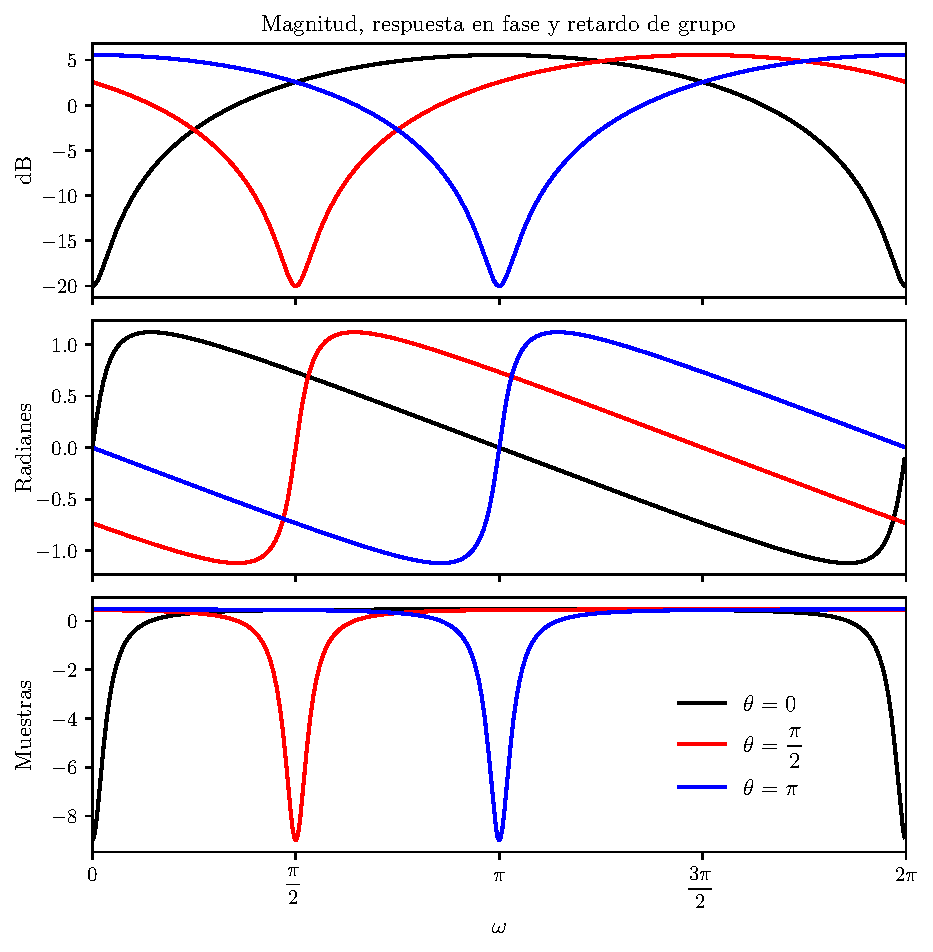
\includegraphics[width=0.9\textwidth]{figuras/transform_analysis_first_order_freq_response_theta.pdf}
 \caption{\label{fig:transform_analysis_first_order_freq_response_theta} Respuesta en frecuencia para un único cero, con \(r=0.9\) y los valores de \(\theta\) indicados en la figura.}
 \end{center}
\end{figure}
Se observa que la magnitud tiene valles en \(\omega=\theta\). También se aprecia en la respuesta en fase que la fase es nula en \(\omega=\theta\) y tiene pendiente positiva máxima en dicho valor. De forma correspondiente, en las funciones del retardo de grupo se observa que hay un pico negativo en \(\omega=\theta\). 

Las características de la respuesta en frecuencia pueden inferirse a partir del diagrama de ceros y polos del sistema. Cada factor correspondiente a un cero o a un polo puede ser representado en plano \(z\) por un vector desde el cero o polo hasta un punto en la circunferencia unidad. En el caso de un sistema de primer orden de la forma
\[
 H(z)=1-re^{j\theta}z^{-1}=\frac{z-re^{j\theta}}{z},
 \qquad\qquad 
 r<1
\]
el diagrama de ceros y polos se muestra en la figura \ref{fig:transform_analysis_first_order_zplane}.
 \begin{figure}[!htb]
  \begin{minipage}[c]{0.53\textwidth}
    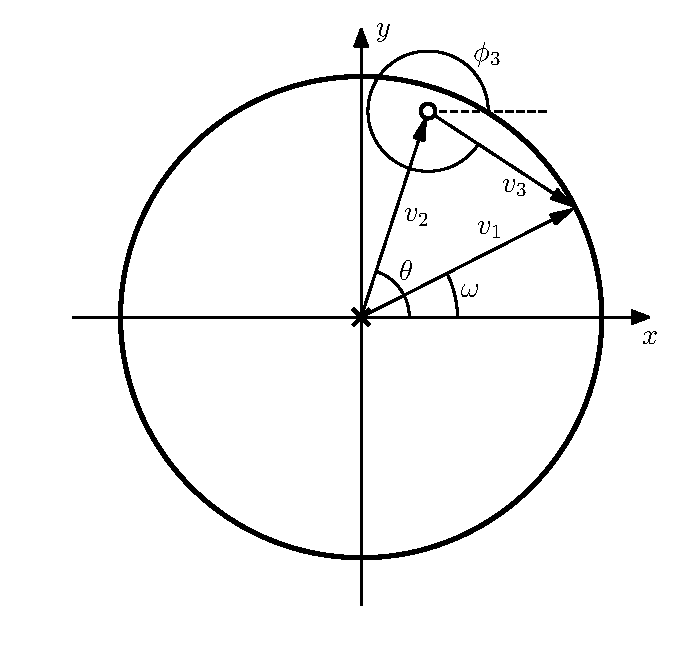
\includegraphics[width=\textwidth]{figuras/transform_analysis_first_order_zplane.pdf}
  \end{minipage}\hfill
  \begin{minipage}[c]{0.38\textwidth}
    \caption{
     Diagrama de polos y ceros de un sistema de primer orden con cero en \(z=re^{j\theta}\) con \(r<1\).
    }\label{fig:transform_analysis_first_order_zplane}
  \end{minipage}
\end{figure}
En la figura se indican los vectores \(v_1\), \(v_2\) y \(v_3=v_1-v_2\) representando los números complejos \(e^{j\omega}\), \(re^{j\theta}\) y \(e^{j\omega}-re^{j\theta}\). La magnitud de la  respuesta en frecuencia del sistema de primer orden en términos de estos vectores es
\[
 |1-re^{j\theta}e^{-j\omega}|=\left|\frac{e^{j\omega}-re^{j\theta}}{e^{j\omega}}\right|=\frac{|v_3|}{|v_1|}=|v_3|.
\]
Esto indica que la contribución de un único factor \(1-re^{j\theta}e^{-j\omega}\) a la magnitud de la respuesta en frecuencia es la longitud del vector \(v_3\) desde el cero al punto \(z=e^{j\omega}\) en la circunferencia unidad. Este vector tiene longitud mínima cuando \(\omega=\theta\), acorde con los valles en la magnitud de la respuesta en frecuencia en la figura \ref{fig:transform_analysis_first_order_freq_response_theta}.
La fase es
\[
 \angle(1-re^{j\theta}e^{-j\omega})=\angle(e^{j\omega}-re^{j\theta})-\angle(e^{j\omega})
  =\angle v_3-\angle v_1=\phi_3-\omega.
\]
Del diagrama de polos y ceros se deduce que cuando \(\omega=\theta\), los vectores \(v_1\), \(v_2\) y \(v_3\) son colineales, y entonces también \(\phi_3=\theta\), resultando en que la fase es nula.

La dependencia del radio \(r\) de la contribución del factor de primer orden a la respuesta en frecuencia se muestra en la figura \ref{fig:transform_analysis_first_order_freq_response_r} para \(\theta=\pi\) y varios valores de \(r\).
\begin{figure}[!htb]
 \begin{center}
 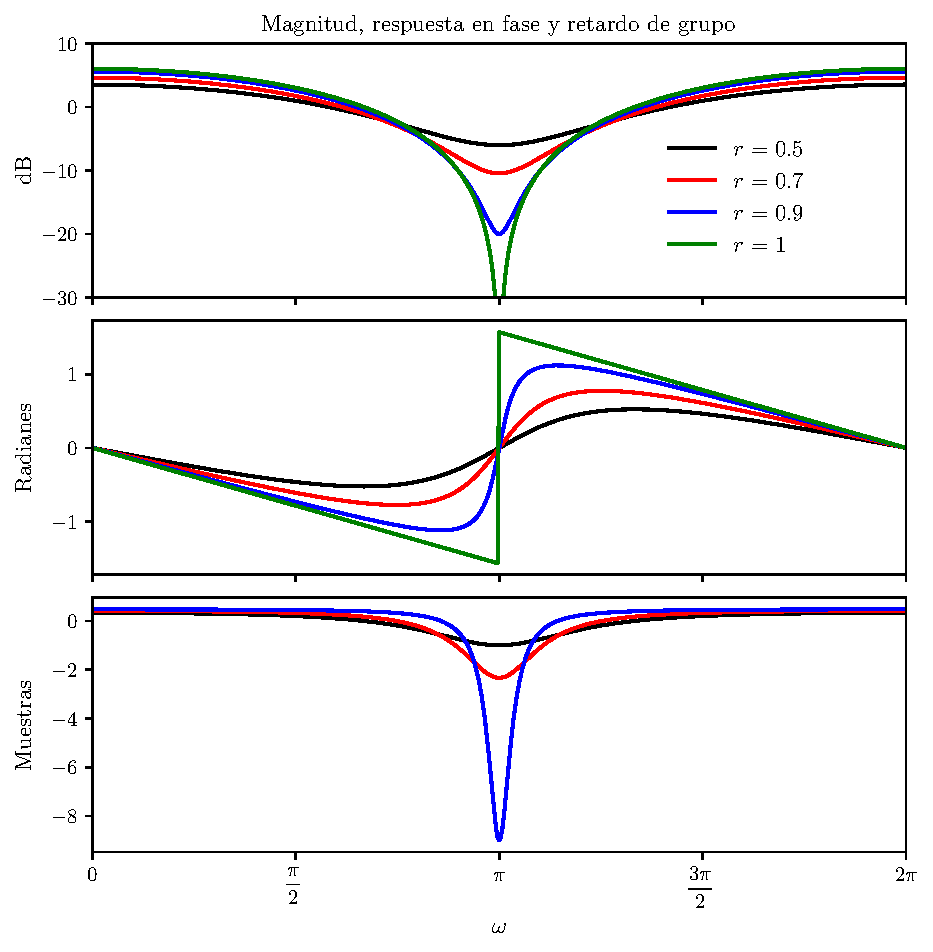
\includegraphics[width=0.9\textwidth]{figuras/transform_analysis_first_order_freq_response_r.pdf}
 \caption{\label{fig:transform_analysis_first_order_freq_response_r} Respuesta en frecuencia para un único cero, con \(\theta=\pi\) y los valores de \(r\) indicados en la figura.}
 \end{center}
\end{figure}
Notar que el valle en la magnitud en decibeles es mas pronunciado a medida que \(r\) se acerca a 1. De hecho, la magnitud en dB tiende a \(-\infty\) en \(\omega=\theta\) cuando \(r\) tiende a 1. La fase tiene pendiente positiva en torno a \(\omega=\theta\), y se hace infinita cuando \(r\) tiende a 1. Es decir, para \(r=1\) la fase es discontinua, con un salto de \(\pi\) radianes en \(\omega=\theta\). El retardo de grupo, que es el opuesto de la pendiente de la fase, tiene un valle cada vez mas pronunciado en \(\omega=\theta\) cuando \(r\) se acerca a 1, y se convierte en un impulso en \(r=1\), no mostrado en la figura. En la figura se aprecia también que el retardo de grupo es relativamente plano en los valores de \(\omega\) lejanos a \(\theta\).

\subsection{Ejemplos con múltiples ceros y polos}

En esta sección se emplea y se expande la discusión de la sección \ref{sec:transform_analysis_first_order_freq_response} para determinar la respuesta en frecuencia de sistemas con función de transferencia racional.

\paragraph{Ejemplo: sistema IIR de segundo orden}

Se considera el sistema de segundo orden
\[
 H(z)=\frac{1}{(1-re^{j\theta}z^{-1})(1-re^{-j\theta}z^{-1})}
  =\frac{1}{1-2r\cos\theta z^{-1}+r^2z^{-2}}.
\]
Se calculará la respuesta al impulso del sistema causal, lo cual puede hacerse mediante el método de descomposición en fracciones simples. La función del sistema puede expresarse en la forma de la ecuación \ref{eq:z_transform_rational_function_simple_fractions_1} como
\[
 H(z)=\frac{A_1}{1-re^{j\theta}z^{-1}}+\frac{A_2}{1-re^{-j\theta}z^{-1}},
\]
donde los coeficientes \(A_1\) y \(A_2\) pueden obtenerse empleando la ecuación \ref{eq:z_transform_rational_function_simple_fractions_A_k}. De esta forma, 
\[
 A_1=(1-re^{j\theta}z^{-1})H(z)\big|_{z=re^{j\theta}}
  =\frac{1}{1-re^{-j\theta}(re^{j\theta})^{-1}}
  =\frac{1}{1-e^{-2j\theta}}
  =\frac{e^{j\theta}}{e^{j\theta}-e^{-j\theta}}
  =\frac{e^{j\theta}}{2j\sen\theta}.
\]
y
\[
 A_2=(1-re^{-j\theta}z^{-1})H(z)\big|_{z=re^{-j\theta}}
  =\frac{1}{1-re^{j\theta}(re^{-j\theta})^{-1}}
  =\frac{1}{1-e^{2j\theta}}
  =\frac{e^{-j\theta}}{e^{-j\theta}-e^{j\theta}}
  =-\frac{e^{-j\theta}}{2j\sen\theta}.
\]
Luego, aplicando la transformada inversa considerando la ROC \(|z|>r\) para que el sistema sea causal (ver la tabla \ref{tab:z_transform_pairs}), se obtiene que 
\begin{align*}
 h[n]&=\frac{e^{j\theta}}{2j\sen\theta}r^ne^{jn\theta}u[n]-\frac{e^{-j\theta}}{2j\sen\theta}r^ne^{-jn\theta}u[n]\\
  &=\frac{r^n}{\sen\theta}\left[\frac{e^{j(n+1)\theta}-e^{-j(n+1)\theta}}{2j}\right]u[n]
\end{align*}
resultando en
\[
 h[n]=\frac{r^n\sen[(n+1)\theta]}{\sen\theta}u[n]
\]
La función del sistema tiene un par de polos complejos conjugados en \(z=re^{\pm j\theta}\) y dos ceros en \(z=0\). El diagrama de polos y ceros se muestra en la figura \ref{fig:transform_analysis_second_order_zplane}. 
 \begin{figure}[!htb]
  \begin{minipage}[c]{0.53\textwidth}
    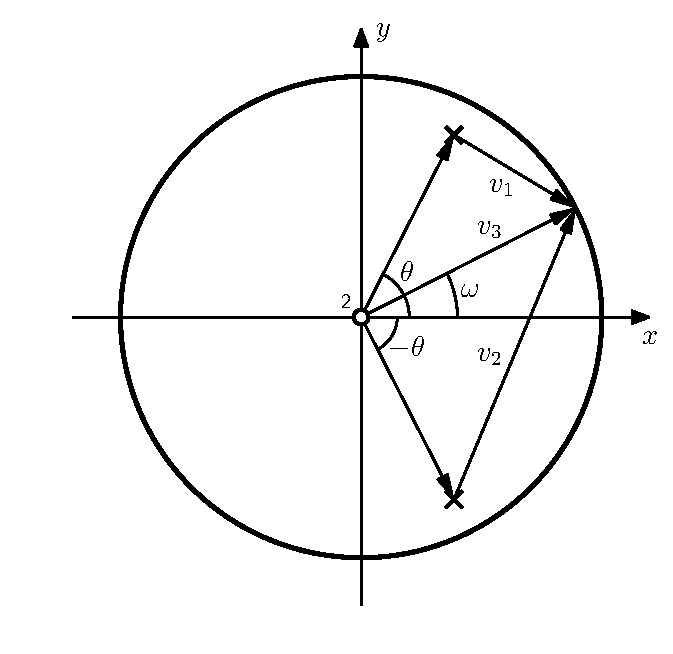
\includegraphics[width=\textwidth]{figuras/transform_analysis_second_order_zplane.pdf}
  \end{minipage}\hfill
  \begin{minipage}[c]{0.38\textwidth}
    \caption{
     Diagrama de polos y ceros del sistema de segundo orden con polos en \(z=re^{\pm j\theta}\) con \(r<1\).
    }\label{fig:transform_analysis_second_order_zplane}
  \end{minipage}
\end{figure}
De los resultados de la sección \ref{sec:transform_analysis_first_order_freq_response} se deduce que la respuesta en magnitud en dB es
\[
 20\log_{10}|H(e^{j\omega})|=-10\log_{10}[1+r^2-2r\cos(\omega-\theta)]-10\log_{10}[1+r^2-2r\cos(\omega+\theta)], 
\]
la respuesta en fase es
\[
  \angle H(e^{j\omega})=-\arctan\left[\frac{r\sen(\omega-\theta)}{1-r\cos(\omega-\theta)}\right]-\arctan\left[\frac{r\sen(\omega+\theta)}{1-r\cos(\omega+\theta)}\right] 
\]
y el retardo de grupo es
\[
 \grd H(e^{j\omega})=-\dfrac{r^2-r\cos(\omega-\theta)}{1+r^2-2r\cos(\omega-\theta)}-\dfrac{r^2-r\cos(\omega+\theta)}{1+r^2-2r\cos(\omega+\theta)}.
\]
Estas funciones se muestran en la figura \ref{fig:transform_analysis_second_order_freq_response_theta} para el valor de \(r=0.9\) y varios valores de \(\theta\).
\begin{figure}[!htb]
 \begin{center}
 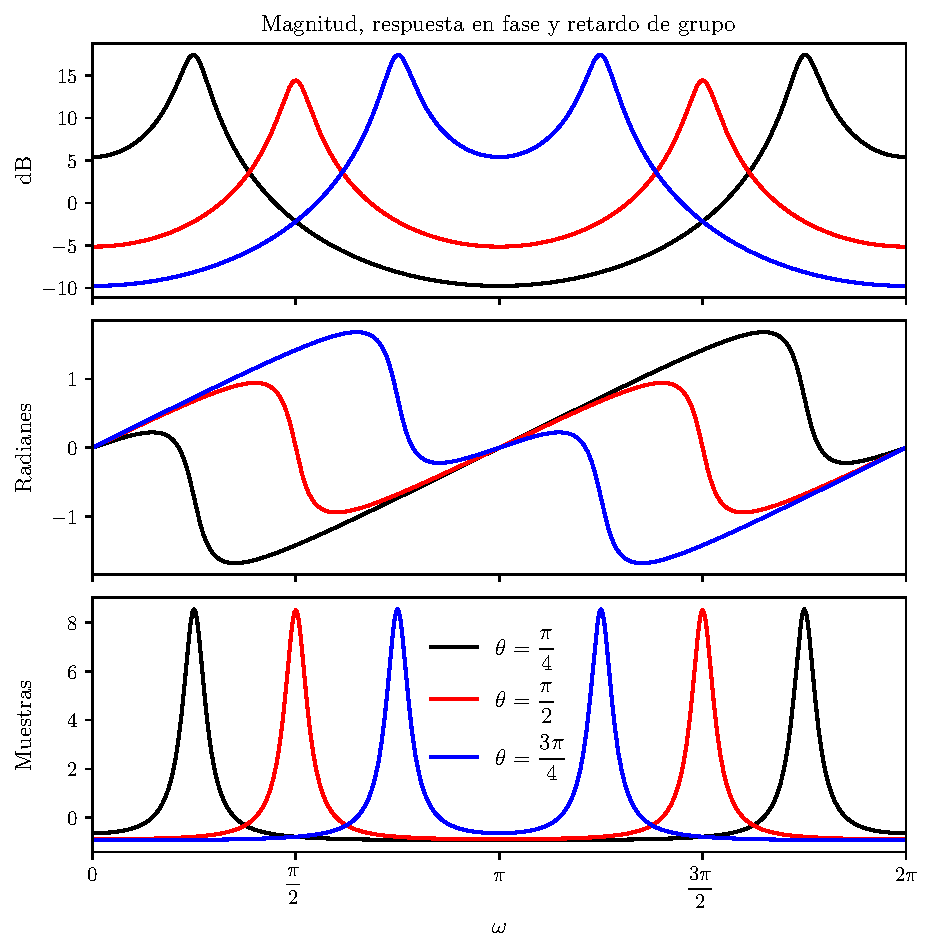
\includegraphics[width=0.9\textwidth]{figuras/transform_analysis_second_order_freq_response_theta.pdf}
 \caption{\label{fig:transform_analysis_second_order_freq_response_theta} Respuesta en frecuencia del sistema de segundo orden, con \(r=0.9\) y los valores de \(\theta\) indicados en la figura.}
 \end{center}
\end{figure}
La figura \ref{fig:transform_analysis_second_order_zplane} muestra los vectores de ceros y polos \(v_1\), \(v_2\) y \(v_3\). La respuesta en magnitud puede expresarse en función de estos vectores como
\[
 |H(e^{j\omega})|=\frac{|e^{j\omega}|^2}{|e^{j\omega}-re^{j\theta}||e^{j\omega}-re^{-j\theta}|}
 =\frac{|v_3|^2}{|v_1||v_2|}=\frac{1}{|v_1||v_2|}.
\]
Esto indica que la respuesta en magnitud es el producto de las longitudes de los vectores de los ceros, que en este caso son la unidad, dividido el producto de los vectores de los polos. Cuando \(\omega\approx\theta\), la longitud del vector \(v_1=e^{j\omega}-re^{j\theta}\) se hace pequeña y cambia significativamente cuando \(\omega\) varía en torno a \(\theta\), mientras que la longitud del vector \(v_2=e^{j\omega}-re^{-j\theta}\) no cambia significativamente cuando \(\omega\) varía en torno a \(\theta\). Por lo tanto, el polo con ángulo \(\theta\) domina en la respuesta en frecuencia en torno a \(\omega=\theta\), como se observa en la respuesta en magnitud en la figura \ref{fig:transform_analysis_second_order_freq_response_theta}. Por simetría, el polo con ángulo \(-\theta\) domina en la respuesta en frecuencia en torno a \(\omega=-\theta\).

\section{Relación entre la magnitud y la fase}\label{sec:transform_analysis_magnitude_and_phase_relation}

En general el conocimiento de la magnitud de la respuesta en frecuencia de un sistema LTI no brinda conocimiento de la fase y viceversa. Sin embargo, para sistemas descritos por ecuaciones en diferencias, es decir, para sistemas con función del sistema racional, hay algunas restricciones entre la magnitud y la fase. En particular, como se verá en esta sección, si se conoce la magnitud de la respuesta en frecuencia y el número de polos y ceros, hay solo una cantidad finita de posibilidades de la fase asociada. De forma similar, si se conoce la cantidad de polos y ceros y la fase, hay solo un número finito de elecciones de la magnitud, salvo un factor de escala. Es mas, si se impone la restricción referida como fase mínima, la magnitud de la respuesta en frecuencia especifica a la fase unívocamente y la respuesta en fase especifica a la respuesta en magnitud excepto por un factor de escala.

Para explorar las elecciones posibles de la función del sistema dado el cuadrado de la respuesta en magnitud, se parte considerando que 
\begin{align}
 |H(e^{j\omega})|^2&=H(e^{j\omega})H^*(e^{j\omega})\nonumber\\
  &=H(z)H^*(1/z^*)\big|_{z=e^{j\omega}}\label{eq:transform_analysis_square_magnitude_z_transform},
\end{align}
donde la última igualdad proviene de que 
\[
 H^*(1/z^*)=\left[\sum_{n=-\infty}^{\infty}h[n]\left(\frac{1}{z^*}\right)^{-n}\right]^*
   =\sum_{n=-\infty}^{\infty}h^*[n]z^n
\]
y por lo tanto,
\[
 H^*(1/z^*)\big|_{z=e^{j\omega}}=\sum_{n=-\infty}^{\infty}h^*[n]e^{j\omega n}=\left(\sum_{n=-\infty}^{\infty}h[n]e^{-j\omega n}\right)^*=H^*(e^{j\omega}).
\]
Restringiendo a la función del sistema a una función racional, puede expresarse de la forma de la ecuación \ref{eq:transform_analysis_difference_equation_system_function_zp},
\[
 H(z)=\left(\frac{b_0}{a_0}\right)\frac{\prod\limits_{k=1}^M(1-c_kz^{-1})}{\prod\limits_{k=1}^N(1-d_kz^{-1})}
\]
y por lo tanto,
\[
 H^*\left(\frac{1}{z^*}\right)=\left(\frac{b_0}{a_0}\right)\frac{\prod\limits_{k=1}^M(1-c^*_kz)}{\prod\limits_{k=1}^N(1-d^*_kz)}
\]
asumiendo que \(a_0\) y \(b_0\) son reales. Considerando estos resultados, la ecuación \ref{eq:transform_analysis_square_magnitude_z_transform} indica que la magnitud al cuadrado es la evaluación en la circunferencia unidad de la transformada \(z\)
\begin{align}
 C(z)&=H(z)H^*(1/z^*)\nonumber\\
  &=\left(\frac{b_0}{a_0}\right)^2\frac{\prod\limits_{k=1}^M(1-c_kz^{-1})(1-c^*_kz)}{\prod\limits_{k=1}^N(1-d_kz^{-1})(1-d^*_kz)}.\label{eq:transform_analysis_square_magnitude_z_transform_cz}
\end{align}
Si se conoce la expresión de \(|H(e^{j\omega})|^2\) como función de \(e^{j\omega}\), reemplazando \(e^{j\omega}\) por \(z\) se obtiene la expresión de \(C(z)\), y a partir de \(C(z)\) se quiere extraer la mayor cantidad de información posible sobre \(H(z)\). Para hacerlo, se observa que por cada polo \(d_k\) de \(H(z)\) hay un polo de \(C(z)\) en \(d_k\) y en \((d_k^*)^{-1}\), y también por cada cero \(c_k\) de \(H(z)\) hay un cero de \(C(z)\) en \(c_k\) y en \((c_k^*)^{-1}\). En consecuencia, los polos y ceros de \(C(z)\) ocurren en pares conjugados inversos, donde un elemento del par lo contribuye \(H(z)\) y el otro lo contribuye \(H^*(1/z^*)\). Observar que si un elemento del par se encuentra dentro de círculo unidad, entonces el otro se encuentra fuera del círculo unidad. La otra alternativa es que ambos se ubiquen sobre la circunferencia unidad en la misma posición.

Si se asume que \(H(z)\) es la función de un sistema causal y estable, todos sus polos deben estar contenidos dentro del círculo unidad. Por lo tanto, con esta restricción, los polos de \(H(z)\) pueden identificarse de los polos de \(C(z)\). Sin embargo, los ceros de \(H(z)\) no pueden identificarse unívocamente de los polos de \(C(z)\).

\section{Sistemas pasa todo}\label{sec:transform_analysis_all_pass_systems}

Una función estable de la forma
\begin{equation}\label{eq:transform_analysis_all_pass_first_order}
 H_\textrm{ap}(z)=\frac{z^{-1}-a^*}{1-az^{-1}} 
\end{equation}
tiene una respuesta en frecuencia con magnitud independiente de \(\omega\). Esto puede verse escribiendo la respuesta en frecuencia como
\begin{equation}\label{eq:transform_analysis_all_pass_first_order_alt}
 H_\textrm{ap}(e^{j\omega})=\frac{e^{-j\omega}-a^*}{1-ae^{-j\omega}}
  =e^{-j\omega}\frac{1-a^*e^{j\omega}}{1-ae^{-j\omega}} 
\end{equation}
y observando que en la expresión de la derecha, el término \(e^{-j\omega}\) tiene magnitud unidad, y la fracción también tiene magnitud unidad debido a que el numerador y el denominador son complejos conjugados. En consecuencia, \(|H_\textrm{ap}(e^{j\omega})|=1\). Este sistema tiene un polo en \(a\) y un cero en \(1/a^*\), es decir, el polo y el cero son un par de números complejos conjugados inversos. 
Un sistema que tiene la magnitud de la frecuencia constante es referido como sistema pasa todo, y permite pasar a todos los componentes espectrales de la entrada con igual ganancia.

La forma mas general de un sistema pasa todo con respuesta al impulso real es el producto de factores como los de la ecuación \ref{eq:transform_analysis_all_pass_first_order}, con los polos complejos en pares conjugados, es decir,
\begin{equation}\label{eq:transform_analysis_all_pass_generic}
 H_\textrm{ap}(z)=A\prod_{k=1}^{M_r}\frac{z^{-1}-d_k}{1-d_kz^{-1}}\prod_{k=1}^{M_c}\frac{(z^{-1}-e_k^*)(z^{-1}-e_k)}{(1-e_kz^{-1})(1-e^*_kz^{-1})}, 
\end{equation}
donde \(A\) es una constante positiva, \(d_k\) son los polos reales y \(e_k\) son los polos complejos. Para que el sistema sea causal y estable se requiere que \(|d_k|<1\) y \(|e_k|<1\).

La respuesta en frecuencia de un sistema pasa todo general puede expresarse en términos de las respuestas en frecuencia de los sistemas de primer orden que lo componen, dados por la ecuación \ref{eq:transform_analysis_all_pass_first_order}. Para sistema causales, cada término consiste en un único polo dentro de la circunferencia unidad y un cero en la posición conjugada inversa. La respuesta en magnitud de cada término es la unidad, como ya fue mostrado. Con \(a\) expresado en forma polar como \(a=re^{j\theta}\), la función de fase de \ref{eq:transform_analysis_all_pass_first_order} es
\begin{equation}\label{eq:transform_analysis_all_pass_first_order_phase}
 \angle\left[\frac{e^{-j\omega}-re^{-j\theta}}{1-re^{j\theta}e^{-j\omega}}\right]=-\omega-2\arctan\left[\frac{r\sen(\omega-\theta)}{1-r\cos(\omega-\theta)}\right], 
\end{equation}
resultado que surge de expresar la respuesta en frecuencia como en la ecuación \ref{eq:transform_analysis_all_pass_first_order_alt} y considerando el resultado de la ecuación \ref{eq:transform_analysis_first_order_freq_response_phase} teniendo en cuenta que la función arcotangente es impar. De forma análoga se deduce que la fase de un sistema de pasa todo de segundo orden con polos en \(z=re^{j\theta}\) y \(z=re^{-j\theta}\) es
\[
 \angle\left[\frac{(e^{-j\omega}-re^{-j\theta})(e^{-j\omega}-re^{j\theta})}{(1-re^{j\theta}e^{-j\omega})(1-re^{-j\theta}e^{-j\omega})}\right]=-\omega-2\arctan\left[\frac{r\sen(\omega-\theta)}{1-r\cos(\omega-\theta)}\right]
 -2\arctan\left[\frac{r\sen(\omega+\theta)}{1-r\cos(\omega+\theta)}\right],
\]

\paragraph{Ejemplo: sistemas pasa todo de primer y segundo orden} La figura \ref{fig:transform_analysis_all_pass_first_second_order} muestra las características de la respuesta en frecuencia de dos sistemas pasa todo de primer orden, uno con el polo en \(z=0.9\) y otro con el polo en \(z=-0.9\). También se muestra la repuesta en frecuencia de un sistema pasa todo de segundo orden con polos en \(z=0.9e^{j\pi/4}\) y \(z=0.9e^{-j\pi/4}\).
\begin{figure}[!htb]
 \begin{center}
 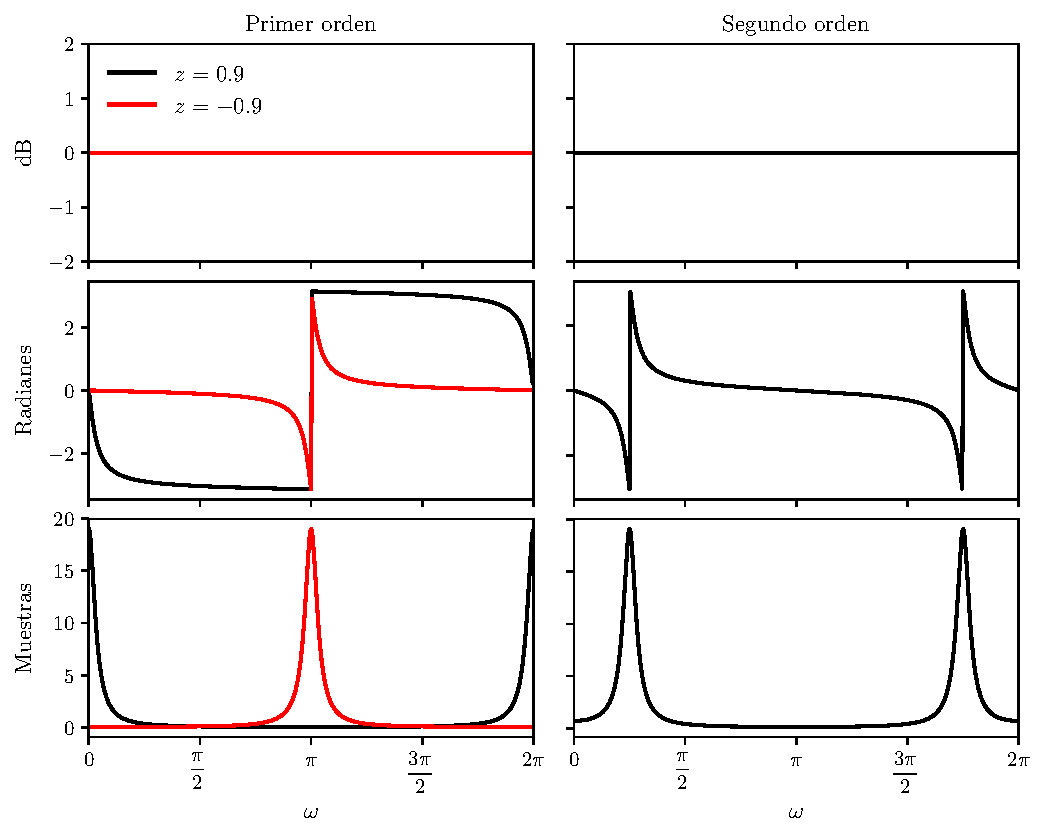
\includegraphics[width=1\textwidth]{figuras/transform_analysis_all_pass_first_second_order.pdf}
 \caption{\label{fig:transform_analysis_all_pass_first_second_order} Sistemas pasa todo. Respuesta en magnitud, respuesta en fase y retardo de grupo de sistemas pasa todo de primer y segundo orden.}
 \end{center}
\end{figure}

El ejemplo ilustra una propiedad general de los sistemas pasa todo. En la figura \ref{fig:transform_analysis_all_pass_first_second_order} se observa que si se eliminan las discontinuidades de \(2\pi\) radianes que se producen en la frecuencia de los polos en la respuesta en fase, la respuesta en fase es no positiva en el intervalo \(0<\omega<\pi\), o en otra palabras, la fase desenrollada es no negativa en dicho intervalo. Como el pasa todo general dado por la ecuación \ref{eq:transform_analysis_all_pass_generic} es el producto de sistemas pasa todo de primer y segundo orden, es posible concluir que la respuesta en fase desenvuelta \(\arg[H_\textrm{ap}(e^{j\omega})]\) de un sistema pasa todo causal es siempre no positiva en \(0<\omega<\pi\). Este resultado puede establecerse analíticamente considerando el retardo de grupo. El retardo de grupo del sistema pasa todo de primer orden \ref{eq:transform_analysis_all_pass_first_order} es la función opuesta a la derivada de la fase, dada por la ecuación \ref{eq:transform_analysis_all_pass_first_order_phase}, es decir,
\begin{align*}
 \grd\left[\frac{e^{-j\omega}-re^{-j\theta}}{1-re^{j\theta}e^{-j\omega}}\right]
   &=-\frac{d}{d\omega}\angle\left[\frac{e^{-j\omega}-re^{-j\theta}}{1-re^{j\theta}e^{-j\omega}}\right]\\
   &\overset{(a)}{=}1-2\left[\dfrac{r^2-r\cos(\omega-\theta)}{1+r^2-2r\cos(\omega-\theta)}\right]\\ 
   &=\dfrac{1+r^2-2r\cos(\omega-\theta)-2r^2+2r\cos(\omega-\theta)}{1+r^2-2r\cos(\omega-\theta)}\\
   &=\dfrac{1-r^2}{1+r^2-2r\cos(\omega-\theta)},
\end{align*}
donde en \((a)\) se empleó el resultado de la ecuación \ref{eq:transform_analysis_first_order_freq_response_grd_alt}. Finalmente, considerando el resultado de la ecuación \ref{eq:transform_analysis_first_order_freq_response_magnitude_alt}, resulta en que 
\begin{equation}\label{eq:transform_analysis_all_pass_first_order_grd}
 \grd\left[\frac{e^{-j\omega}-re^{-j\theta}}{1-re^{j\theta}e^{-j\omega}}\right]=\dfrac{1-r^2}{1+r^2-2r\cos(\omega-\theta)}=\frac{1-r^2}{|1-re^{j\theta}e^{-j\omega}|^2}.
\end{equation}
Como \(r<1\) para un sistema pasa todo causal y estable, el retardo de grupo contribuido por un único factor pasa todo es siempre positivo. Como el retardo de grupo de sistemas pasa todo de mayor orden es la suma de los retardos de grupo de los factores de primer orden, será siempre positivo en general.  

La positividad del retardo de grupo de los sistemas pasa todo causales es la base de una prueba simple de la no negatividad de la fase de dichos sistemas. Efectivamente, de la definición de retardo de grupo y el teorema fundamental del cálculo, se cumple que 
\begin{equation}\label{eq:transform_analysis_argument_grd_relation_fundamental}
 \arg[H_\textrm{ap}(e^{j\omega})]=-\int_0^\omega\grd[H_\textrm{ap}(e^{j\phi})]\,d\phi+\arg[H_\textrm{ap}(e^{j0})] 
\end{equation}
en el intervalo \(0<\omega<\pi\). De la ecuación \ref{eq:transform_analysis_all_pass_generic},
\[
 \arg[H_\textrm{ap}(e^{j0})]=A\prod_{k=1}^{M_r}\frac{1-d_k}{1-d_k}\prod_{k=1}^{M_c}\frac{(1-e_k^*)(1-e_k)}{(1-e_k)(1-e^*_k)}=A\prod_{k=1}^{M_r}\frac{1-d_k}{1-d_k}\prod_{k=1}^{M_c}\frac{|1-e_k|^2}{|1-e_k|^2}=A.
\]
Por lo tanto, \(\arg[H_\textrm{ap}(e^{j0})]=0\), y como
\[
 \grd[H_\textrm{ap}(e^{j\omega})]\geq0
\]
de la ecuación \ref{eq:transform_analysis_argument_grd_relation_fundamental} se concluye que 
\[
 \arg[H_\textrm{ap}(e^{j\omega})]\leq0
 \qquad\qquad\textrm{para}\qquad\qquad
 0\leq\omega<\pi.
\]
La positividad del retardo de grupo y la no positividad de la fase desenrollada son propiedades importantes de los sistemas pasa todo causales.

Los sistemas pasa todo tienen importancia en diversos contextos. Pueden emplearse para contrarrestar el efecto de la distorsión de fase. También son útiles para transformar filtros pasabajos en los otros tipos de filtros de selección de frecuencias. Estos aspectos se verán en el capítulo \ref{}. Además, también son útiles en la teoría de los sistemas de fase mínima, como se verá en la sección \ref{sec:transform_analysis_minimum_phase_systems}

\section{Sistemas de fase mínima}\label{sec:transform_analysis_minimum_phase_systems}

En la sección \ref{sec:transform_analysis_magnitude_and_phase_relation} se mostró que la magnitud de la respuesta en frecuencia de un sistema LTI con función del sistema racional no caracteriza unívocamente al sistema. Si el sistema es causal y estable, los polos deben estar dentro de la circunferencia unidad, pero dichas condiciones no imponen restricciones sobre los ceros. En ciertas clases de problemas es útil imponer la condición adicional de que el sistema inverso también sea causal y estable. Como se discutió en la sección \ref{sec:transform_analysis_inverse_systems}, esta condición restringe a que tanto los polos como los ceros estén contenidos en el círculo unidad. Esta clase de sistemas es referida como \emph{sistemas de fase mínima}. El nombre fase mínima proviene de una propiedad de la respuesta en fase que no es obvia a partir de la definición precedente. Esta y otras propiedades, que se verán en esta sección, son únicas de esta clase de sistemas y por lo tanto, cada una de ellas puede considerarse como la definición de la clase.

Si se conoce el cuadrado de la respuesta en magnitud en la forma de la ecuación \ref{eq:transform_analysis_square_magnitude_z_transform_cz} y se sabe que tanto el sistema como el sistema inverso son causales y estables, \(H(z)\) queda unívocamente determinado y consistirá en los polos y ceros de \(C(z)=H(z)H^*(1/z^*)\) contenidos dentro del círculo unidad. Este enfoque es empleado en diseño de filtros cuando únicamente es especificada la respuesta en magnitud por el método de diseño empleado (ver el capítulo \ref{}).

\subsection{Descomposición en fase mínima y pasa todo}\label{sec:transform_analysis_min_phase_all_pass_decomposition}

En la sección \ref{sec:transform_analysis_magnitude_and_phase_relation} se vio que a partir de la respuesta en magnitud al cuadrado no es posible determinar unívocamente la función del sistema \(H(z)\), ya que cualquier elección de respuesta en frecuencia con la magnitud dada puede ponerse en cascada con un número arbitrario de factores pasa todo sin afectar la magnitud. Una observación relacionada es que cualquier función del sistema racional puede expresarse como
\begin{equation}\label{eq:transform_analysis_min_phase_all_pass_decomposition}
 H(z)=H_\textrm{min}(z)H_\textrm{ap}(z), 
\end{equation}
donde \(H_\textrm{min}(z)\) es un sistema de fase mínima y \(H_\textrm{ap}(z)\) es un sistema pasa todo.

Para mostrar esto, supóngase que \(H(z)\) tiene un cero fuera del círculo unidad en \(z=1/c^*\), donde \(|c|<1\), y el resto de los polos y ceros se encuentran dentro del círculo unidad. De esta forma, \(H(z)\) puede expresarse como
\begin{equation}\label{eq:transform_analysis_min_phase_all_pass_decomposition_tmp1}
 H(z)=H_1(z)(z^{-1}-c^*), 
\end{equation}
donde por definición, \(H_1(z)\) es de fase mínima. Una expresión equivalente para \(H(z)\) es
\begin{equation}\label{eq:transform_analysis_min_phase_all_pass_decomposition_tmp2}
 H(z)=H_1(z)(1-cz^{-1})\frac{z^{-1}-c^*}{1-cz^{-1}}. 
\end{equation}
Como \(|c|<1\), el factor \(H_1(z)(1-cz^{-1})\) es de fase mínima y difiere de \(H(z)\) únicamente en que el cero de \(H(z)\) que estaba fuera del círculo unidad en \(z=1/c^*\) fue reflejado dentro del círculo unidad a la posición conjugada inversa \(z=c\). El factor \((z^{-1}-c^*)/(1-cz^{-1})\) es pasa todo. El ejemplo puede generalizarse para incluir mas ceros fuera del círculo unidad. Por lo tanto, en la ecuación \ref{eq:transform_analysis_min_phase_all_pass_decomposition}, \(H_\textrm{min}(z)\) contiene todos los polos y ceros de \(H(z)\) contenidos dentro del círculo unidad, y además, ceros en la posición conjugada inversa de los ceros de \(H(z)\) fuera del círculo unidad. El sistema \(H_\textrm{ap}(z)\) se compone de todos los ceros de \(H(z)\) fuera del círculo unidad y polos en la posición conjugada inversa que se cancelan con los ceros que fueron reflejados hacia adentro del círculo unidad en \(H_\textrm{min}(z)\).

Mediante la ecuación \ref{eq:transform_analysis_min_phase_all_pass_decomposition} se puede construir un sistema de fase no mínima a partir de un sistema de fase mínima reflejando uno o mas ceros dentro del círculo unidad a la posición conjugada inversa fuera del círculo unidad, o viceversa, se puede construir un sistema de fase mínima a partir de un sistema de fase no mínima reflejando los ceros fuera del círculo unidad a la posición conjugada inversa dentro del círculo unidad. En ambos casos, el sistema de fase mínima y el sistema de fase no mínima tienen la misma respuesta en magnitud.

\paragraph{Ejemplo: descomposición en fase mínima y pasa todo} Considérese el sistema
\[
 H(z)=\dfrac{\left(1+\dfrac{3}{2}e^{j\pi/4}z^{-1}\right)\left(1+\dfrac{3}{2}e^{-j\pi/4}z^{-1}\right)}{1-\dfrac{1}{3}z^{-1}}.
\]
Este sistema tiene dos ceros complejos en 
\[
 z=\frac{3}{2}e^{-j3\pi/4}
 \qquad\textrm{y}\qquad
 z=\frac{3}{2}e^{j3\pi/4}
\]
fuera del círculo unidad y un polo real en \(z=1/3\) dentro del círculo unidad. \(H(z)\) puede expresarse en la forma de la ecuación \ref{eq:transform_analysis_min_phase_all_pass_decomposition_tmp1} como
\begin{align*}
  H(z)&=\dfrac{\dfrac{3}{2}e^{j\pi/4}\left(\dfrac{2}{3}e^{-j\pi/4}+z^{-1}\right)\dfrac{3}{2}e^{-j\pi/4}\left(\dfrac{2}{3}e^{j\pi/4}+z^{-1}\right)}{1-\dfrac{1}{3}z^{-1}}\\
   &=\frac{9}{4}\dfrac{\left(z^{-1}+\dfrac{2}{3}e^{-j\pi/4}\right)\left(z^{-1}+\dfrac{2}{3}e^{j\pi/4}\right)}{1-\dfrac{1}{3}z^{-1}},
\end{align*}
y factorizando como en la ecuación \ref{eq:transform_analysis_min_phase_all_pass_decomposition_tmp2} se obtiene que 
\[
 H(z)=\underbrace{\left[\frac{9}{4}\dfrac{\left(1+\dfrac{2}{3}e^{j\pi/4}z^{-1}\right)\left(1+\dfrac{2}{3}e^{-j\pi/4}z^{-1}\right)}{1-\dfrac{1}{3}z^{-1}}\right]}_{\displaystyle H_\textrm{min}(z)}
 \underbrace{\left[\dfrac{\left(z^{-1}+\dfrac{2}{3}e^{-j\pi/4}\right)\left(z^{-1}+\dfrac{2}{3}e^{j\pi/4}\right)}{\left(1+\dfrac{2}{3}e^{j\pi/4}z^{-1}\right)\left(1+\dfrac{2}{3}e^{-j\pi/4}z^{-1}\right)}\right]}_{\displaystyle H_\textrm{ap}(z)}.
\]
\begin{figure}[!htb]
 \begin{center}
 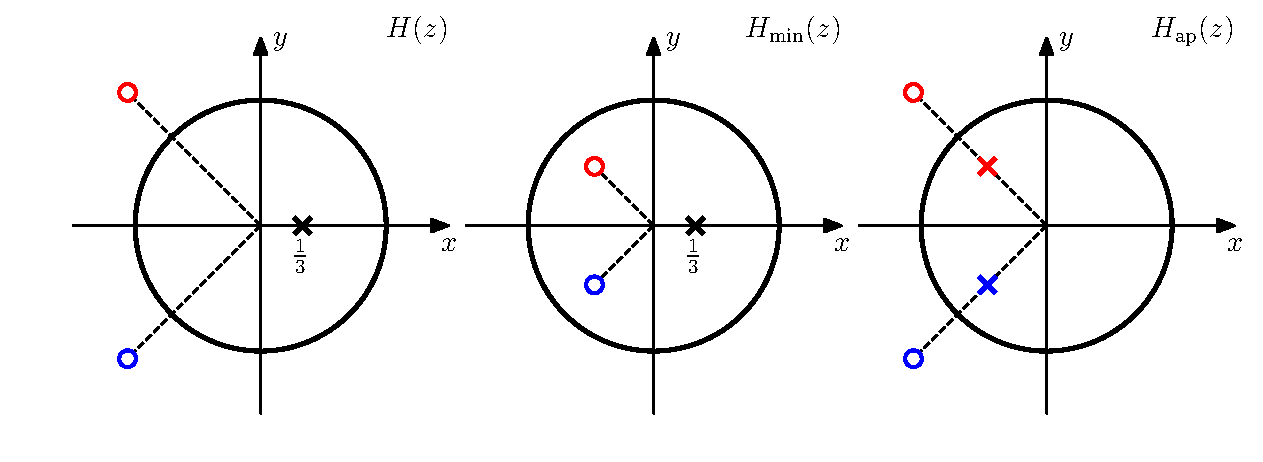
\includegraphics[width=0.97\textwidth]{figuras/example_5_12_zero_pole_plot.pdf}
 \caption{\label{fig:example_5_12_zero_pole_plot} Diagrama de polos y ceros del sistema \(H(z)\) y del sistema de fase mínima \(H_\textrm{min}(z)\) y pasa todo \(H_\textrm{min}(z)\) en que se descompone.}
 \end{center}
\end{figure}
El primer sistema entre paréntesis rectos tiene dos ceros en
\[
 z=\frac{2}{3}e^{-j3\pi/4}
 \qquad\textrm{y}\qquad
 z=\frac{2}{3}e^{j3\pi/4},
\]
que son los reflejos de los ceros de \(H(z)\) fuera del círculo unidad a la posición conjugada inversa dentro del círculo unidad, y un polo en \(z=1/3\) dentro del círculo unidad, y por lo tanto, es de fase mínima. El segundo sistema es un pasa todo, cuyos polos se cancelan con los ceros del sistema de fase mínima. En la figura \ref{fig:example_5_12_zero_pole_plot} se muestra el diagrama de polos de los sistemas \(H(z)\), \(H_\textrm{min}(z)\) y \(H_\textrm{ap}(z)\).

\subsection{Compensación de la respuesta en frecuencia de sistemas de fase no mínima}\label{sec:transform_analysis_non_minimum_phase_compensation}

En muchas aplicaciones de procesamiento de señales ocurre que una señal puede ser distorsionada por un sistema LTI con respuesta en frecuencia no deseada, y es de interés procesar la señal distorsionada con un sistema compensador, como se muestra en la figura \ref{fig:non_minimum_phase_freq_response_compensation}. Si se logra compensación perfecta, \(s_c[n]=s[n]\), o equivalentemente, \(H_c(z)\) es el sistema inverso de \(H_d(z)\). Sin embargo, si se asume que el sistema distorsionador es causal y estable y se requiere que el sistema compensador sea causal y estable, la compensación perfecta solo es posible si \(H_d(z)\) es de fase mínima, de forma tal que tenga un sistema inverso causal y estable.
\begin{figure}[!htb]
 \begin{minipage}[c]{0.53\textwidth}
  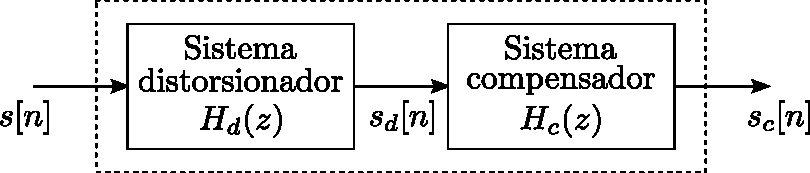
\includegraphics[width=\textwidth]{figuras/non_minimum_phase_freq_response_compensation.pdf}
 \end{minipage}\hfill
 \begin{minipage}[c]{0.37\textwidth}
 \caption{Compensación de la distorsión mediante filtrado.
 }\label{fig:non_minimum_phase_freq_response_compensation}
 \end{minipage}
\end{figure}

En base a lo discutido previamente, asumiendo que \(H_d(z)\) es conocido o aproximado por una función racional, se puede construir un sistema de fase mínima \({H_d}_\textrm{min}(z)\) reflejando todos los ceros de \(H_d(z)\) que están fuera del círculo unidad a las posiciones conjugadas inversas dentro del círculo unidad. De esta forma, \(H_d(z)\) y \({H_d}_\textrm{min}(z)\) tienen la misma magnitud de respuesta en frecuencia y están vinculados mediante un sistema pasa todo \(H_\textrm{ap}(z)\),
\[
 H_d(z)={H_d}_\textrm{min}(z)H_\textrm{ap}(z)
\]
Eligiendo el sistema compensador como
\[
 H_c(z)=\frac{1}{{H_d}_\textrm{min}(z)},
\]
la función del sistema completo entre la entrada \(s[n]\) y la salida \(s_c[n]\) es
\[
 G(z)=H_d(z)H_c(z)=H_\textrm{ap}(z).
\]
es decir, \(G(z)\) corresponde a un sistema pasa todo. En consecuencia, la distorsión en magnitud es perfectamente compensada mientras que la respuesta en fase es modificada como \(\angle H_\textrm{ap}(z)\).

El siguiente ejemplo ilustra la compensación de la magnitud de la respuesta en frecuencia para un sistema FIR.

\paragraph{Ejemplo: compensación para un sistema FIR} Se considera el sistema distorsionador con función del sistema
\begin{equation}\label{eq:transform_analysis_example_5_13_H_d}
 H_d(z)=(1-0.9e^{j0.6\pi}z^{-1})(1-0.9e^{-j0.6\pi}z^{-1})(1-1.25e^{j0.8\pi}z^{-1})(1-1.25e^{-j0.8\pi}z^{-1}). 
\end{equation}
El diagrama de polos y ceros se muestra en la figura \ref{fig:example_5_13_zero_pole_plot}. Como \(H_d(z)\) tiene solo ceros (todos los polos están en \(z=0\)), el sistema tiene respuesta al impulso de duración finita. Por lo tanto, el sistema es estable, y además, como \(H_d(z)\) es un polinomio que tiene solo potencias negativas de \(z\), el sistema es causal. Sin embargo, como el sistema tiene dos ceros fuera del círculo unidad, el sistema no es fase mínima.
\begin{figure}[!htb]
  \begin{minipage}[c]{0.45\textwidth}
    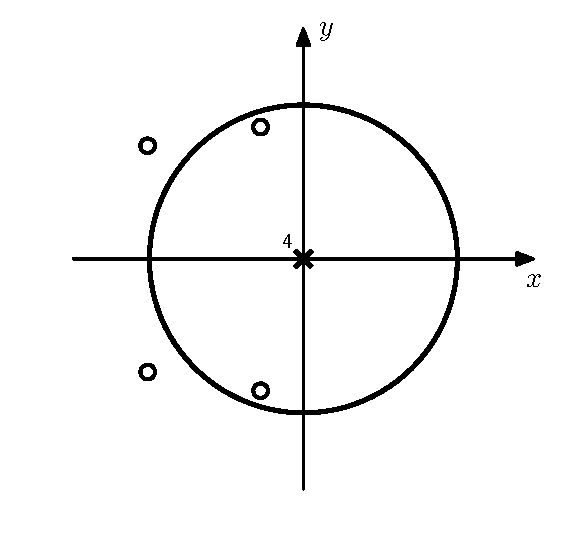
\includegraphics[width=\textwidth]{figuras/example_5_13_zero_pole_plot.pdf}
  \end{minipage}\hfill
  \begin{minipage}[c]{0.45\textwidth}
    \caption{
      Diagrama de polos y ceros del sistema FIR del ejemplo.
    }\label{fig:example_5_13_zero_pole_plot}
  \end{minipage}
\end{figure}

El sistema correspondiente de fase mínima se obtiene reflejando los ceros en \(z=1.25e^{\pm j0.8\pi}\) a sus posiciones inversas conjugadas dentro del círculo unidad. Expresando \(H_d(z)\) como
\begin{align*}
 H_d(z)&=(1-0.9e^{j0.6\pi}z^{-1})(1-0.9e^{-j0.6\pi}z^{-1})1.25e^{j0.8\pi}(0.8e^{-j0.8\pi}-z^{-1})1.25e^{-j0.8\pi}(0.8e^{j0.8\pi}-z^{-1})\\
  &=(1.25)^2(1-0.9e^{j0.6\pi}z^{-1})(1-0.9e^{-j0.6\pi}z^{-1})(z^{-1}-0.8e^{-j0.8\pi})(z^{-1}-0.8e^{j0.8\pi}),
\end{align*}
se deduce que en la descomposición el sistema de fase mínima es
\begin{equation}\label{eq:transform_analysis_example_5_13_H_min}
 {H_d}_\textrm{min}(z)=(1.25)^2(1-0.9e^{j0.6\pi}z^{-1})(1-0.9e^{-j0.6\pi}z^{-1})(1-0.8e^{-j0.8\pi}z^{-1})(1-0.8e^{j0.8\pi}z^{-1}),
 \end{equation}
y el sistema pasa todo es
\begin{equation}\label{eq:transform_analysis_example_5_13_H_ap}
 H_\textrm{ap}(z)=\frac{(z^{-1}-0.8e^{-j0.8\pi})(z^{-1}-0.8e^{j0.8\pi})}{(1-0.8e^{j0.8\pi}z^{-1})(1-0.8e^{-j0.8\pi}z^{-1})}. 
\end{equation}

\begin{figure}[!htb]
 \begin{center}
 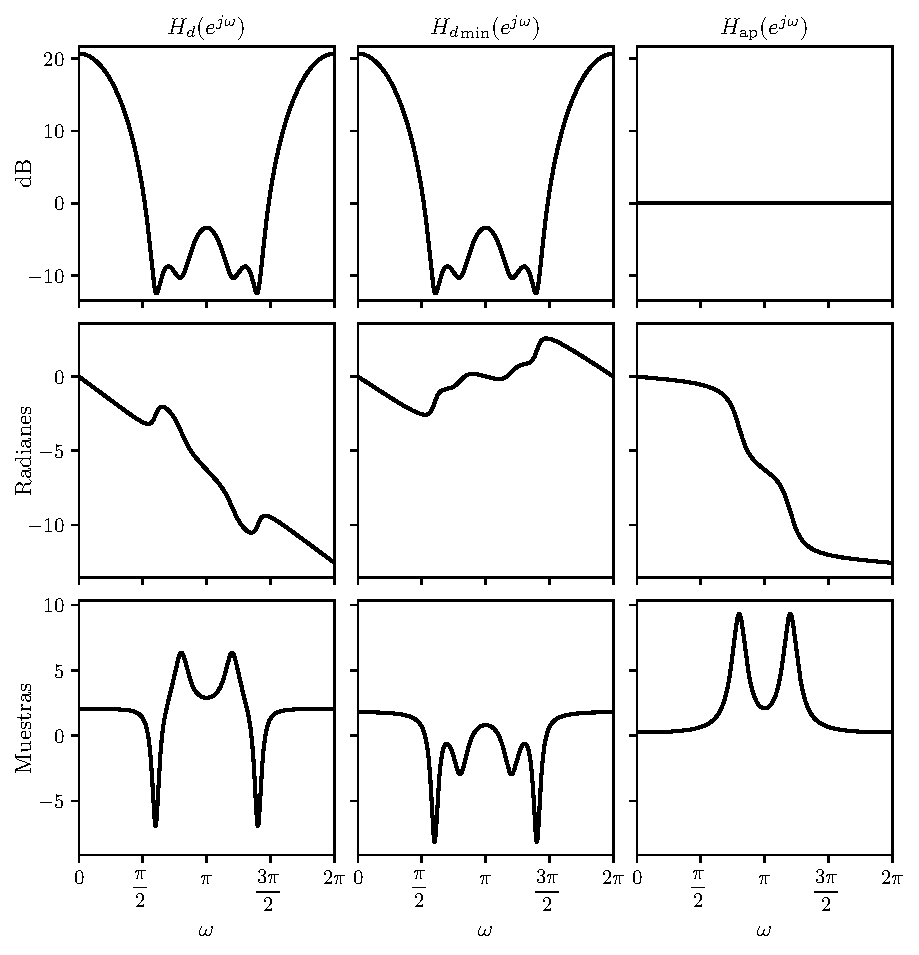
\includegraphics[width=0.97\textwidth]{figuras/example_5_13_H_freq_responses.pdf}
 \caption{\label{fig:transform_analysis_example_5_13_H_freq_responses} Respuesta en magnitud logarítmica, la fase desenrollada y retardo de grupo de los sistemas \(H_d(z)\), \({H_d}_\textrm{min}(z)\) y \(H_\textrm{ap}(z)\).}
 \end{center}
\end{figure}
La respuesta en magnitud logarítmica, la fase desenrollada y el retardo de grupo de \(H_d(e^{j\omega})\), \({H_d}_\textrm{min}(e^{j\omega})\) y \(H_\textrm{ap}(e^{j\omega})\) se muestran en la figura \ref{fig:transform_analysis_example_5_13_H_freq_responses}. Como corresponde, la respuesta en magnitud de \(H_d(e^{j\omega})\) y \({H_d}_\textrm{min}(e^{j\omega})\) son idénticas.
Observar que el sistema inverso de \(H_d(z)\) tiene polos en \(z=1.25e^{\pm j0.8\pi}\) y por lo tanto, el sistema causal inverso sería inestable. El sistema inverso de fase mínima sería el inverso de \({H_d}_\textrm{min}(z)\), dado por la ecuación \ref{eq:transform_analysis_example_5_13_H_min}, y si este sistema inverso fuera empleado como sistema compensador en la figura \ref{fig:non_minimum_phase_freq_response_compensation}, la respuesta global del sistema sería \(H_\textrm{ap}(z)\), dado por la ecuación \ref{eq:transform_analysis_example_5_13_H_ap}.

\subsection{Propiedades de los sistemas de fase mínima}

Se ha empleado el término \emph{fase mínima} para referirse a un sistema causal y estable que tiene un sistema inverso causal y estable. El nombre está motivado por una propiedad de la función de fase de esta clase de sistemas. En esta sección se discuten las propiedades de los sistemas de fase mínima en comparación con otros sistemas con la misma magnitud de respuesta en frecuencia.

\subsubsection{Propiedad de disminución de fase mínima}

El término sistema de fase mínima como nombre descriptivo de los sistemas que tienen todos los polos y ceros dentro del círculo unidad está sugerido por el ejemplo de la sección \ref{sec:transform_analysis_non_minimum_phase_compensation}. Como consecuencia de la ecuación \ref{eq:transform_analysis_min_phase_all_pass_decomposition}, la fase desenrollada de un sistema de fase no mínima puede expresarse como
\[
 \arg[H(e^{j\omega})]=\arg[H_\textrm{min}(e^{j\omega})]+\arg[H_\textrm{ap}(e^{j\omega})].
\]
Por ejemplo, en la figura \ref{fig:transform_analysis_example_5_13_H_freq_responses}, la función de fase de \(H_d(e^{j\omega})\) es la suma de la función de fase de \({H_d}_\textrm{min}(e^{j\omega})\) y la función de fase de \(H_\textrm{ap}(e^{j\omega})\). Como se mostró en la sección \ref{sec:transform_analysis_all_pass_systems} y se observa en las gráficas de la respuesta en fase en las figuras \ref{fig:transform_analysis_all_pass_first_second_order} y \ref{fig:transform_analysis_example_5_13_H_freq_responses}, las fase desenrollada de los sistemas pasa todo es negativa en \(0\leq\omega\leq\pi\). Por lo tanto, la reflexión de los ceros de \(H_\textrm{min}(z)\) dentro del círculo unidad a su posición conjugada inversa fuera del círculo unidad producida por el sistema pasa todo siempre disminuye la respuesta en fase desenrollada o incrementa el negativo de fase, que se llama función de \emph{disminución de fase}. De esta forma, el sistema causal y estable que tiene a \(|H_\textrm{min}(e^{j\omega})|\) como magnitud de la respuesta en frecuencia tiene la mínima función de disminución de fase de todos los sistemas con la misma respuesta en magnitud, como se observa en la función de fase de \({H_d}_\textrm{min}(e^{j\omega})\) en la figura \ref{fig:transform_analysis_example_5_13_H_freq_responses}. Entonces, una terminología mas precisa sería sistema de \emph{disminución de fase mínima}, pero sistema de \emph{fase mínima} es el término establecido históricamente.

Para hacer mas precisa la interpretación de sistema de disminución de fase mínima, es necesario imponer la restricción adicional de que \(H(e^{j\omega})\) sea positivo en \(\omega=0\), es decir,
\[
 H(e^{j0})=\sum_{n=-\infty}^\infty h[n]>0.
\]
Notar que \(H(e^{j0})\) es real si \(h[n]\) es real. Esta condición es necesaria debido a que un sistema con respuesta al impulso \(-h[n]\) tiene los mismos polos y ceros que un sistema con respuesta al impulso \(h[n]\). Sin embargo, la multiplicación por \(-1\) altera la fase en \(\pi\) radianes. Así, para eliminar esta ambigüedad y asegurar que el sistema con los polos y ceros dentro del círculo unidad sea el que tiene disminución de fase mínima se impone la condición \(H(e^{j0})>0\). Esta condición es de poca importancia, y la definición al comienzo de esta sección, que es la definición aceptada de sistemas de fase mínima, no la incluye.

\subsubsection{Propiedad de retardo de grupo mínimo} 

El ejemplo de la sección \ref{sec:transform_analysis_non_minimum_phase_compensation} ilustra otra propiedad de los sistemas con los polos y ceros dentro del círculo unidad. Nuevamente, como consecuencia de la ecuación  \ref{eq:transform_analysis_min_phase_all_pass_decomposition}, para dos sistemas con la misma magnitud de respuesta en frecuencia se cumple que 
\[
 \grd[H(e^{j\omega})]=\grd[H_\textrm{min}(e^{j\omega})]+\grd[H_\textrm{ap}(e^{j\omega})].
\]
El retardo de grupo del sistema de fase mínima es siempre menor que el retado de grupo del sistema con fase no mínima, como se observa en la figura \ref{fig:transform_analysis_example_5_13_H_freq_responses}. Esto es porque el sistema pasa todo que convierte al sistema de fase mínima en el sistema de fase no mínima tiene retardo de grupo positivo, como se aprecia en la figura \ref{fig:transform_analysis_example_5_13_H_freq_responses} para el ejemplo. Como se mostró en la sección \ref{sec:transform_analysis_all_pass_systems}, el retardo de grupo positivo es una propiedad de todos los sistemas pasa todo (ver también la figura \ref{fig:transform_analysis_all_pass_first_second_order}). Se concluye que entre todos los sistemas con una magnitud de respuesta en frecuencia \(|H_\textrm{min}(e^{j\omega})|\) dada, el que tiene todos los polos y ceros dentro del círculo unidad es el de retardo de grupo mínimo. Un nombre apropiado para estos sistemas sería también sistemas de \emph{retardo de grupo mínimo}, pero este término no es usado en general.

\subsubsection{Propiedad de retardo de energía mínimo} 

En el ejemplo de la sección \ref{sec:transform_analysis_non_minimum_phase_compensation} hay un total de cuatro sistemas FIR causales con respuesta al impulso real que tienen la misma magnitud de respuesta en frecuencia que el sistema dado por la ecuación \ref{eq:transform_analysis_example_5_13_H_d}. Los diagramas de polos y ceros asociados se muestran en la figura \ref{fig:example_5_13_minimum_energy_zero_pole_plot}, donde \(H_d(z)\) corresponde al sistema de la ecuación \ref{eq:transform_analysis_example_5_13_H_d} y el sistema \(H_a(z)\) corresponde al sistema de fase mínima de la ecuación \ref{eq:transform_analysis_example_5_13_H_min}. 
\begin{figure}[!htb]
 \begin{center}
 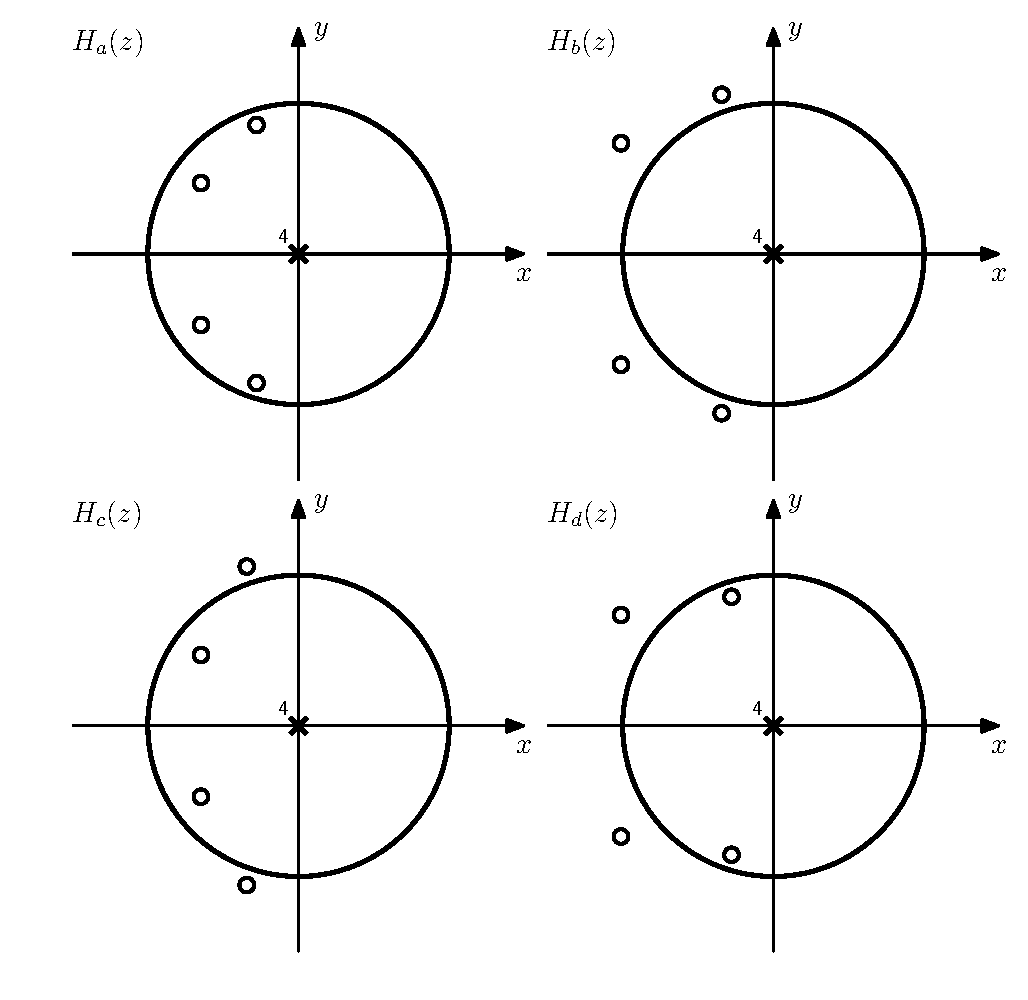
\includegraphics[width=0.8\textwidth]{figuras/example_5_13_minimum_energy_zero_pole_plot.pdf}
 \caption{\label{fig:example_5_13_minimum_energy_zero_pole_plot} Diagrama de polos y ceros de cuatro sistemas que tienen la misma magnitud de respuesta en frecuencia. Los ceros son todas las combinaciones de los pares de ceros conjugados \(0.9e^{\pm j0.6\pi}\) y \(0.8e^{\pm j0.8\pi}\) y los inversos.}
 \end{center}
\end{figure}
Las respuestas al impulso de los cuatro sistemas se muestran en la figura \ref{fig:example_5_13_minimum_energy_impulse_responses}. Si se comparan las cuatro secuencias de la figura, se observa que la secuencia de fase mínima parecería tener muestras mas grandes en el lado izquierdo que el resto de las secuencias.
\begin{figure}[!htb]
 \begin{center}
 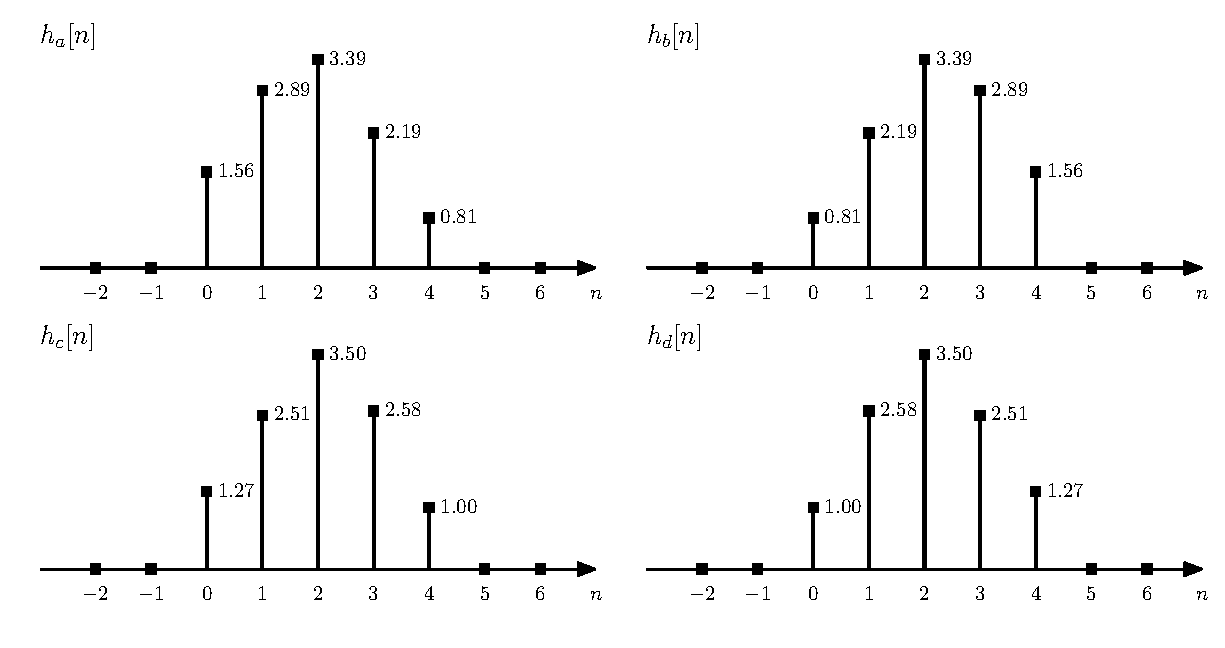
\includegraphics[width=1\textwidth]{figuras/example_5_13_minimum_energy_impulse_responses.pdf}
 \caption{\label{fig:example_5_13_minimum_energy_impulse_responses} Secuencias correspondientes a los sistemas de con diagrama de polos y ceros de la figura \ref{fig:example_5_13_minimum_energy_zero_pole_plot}.}
 \end{center}
\end{figure}
Esto es cierto para este ejemplo, y también en general. En general, siempre se cumple que 
\[
 |h[0]|\leq |h_\textrm{min}[0]|
\]
para cualquier secuencia \(h[n]\) causal y estable tal que 
\[
 |H(e^{j\omega})|=|H_\textrm{min}(e^{j\omega})|.
\]
Para la prueba (ver el problema 5.71 de \cite{oppenheim2009discrete}), se parte considerando que cualquier sistema de fase no mínima puede expresarse como la cascada del sistema de fase mínima y un sistema pasa todo. Por lo tanto, el sistema \(H(z)\) puede escribirse como 
\[
 H(z)=H_\textrm{min}(z)H_\textrm{ap}(z),
\]
donde \(H_\textrm{min}(z)\) y \(H_\textrm{ap}(z)\) se obtienen mediante el reflejo de los ceros fuera del círculo unidad, como se discutió en la sección \ref{sec:transform_analysis_min_phase_all_pass_decomposition}. Tomado el límite para \(z\) tendiendo a infinito en ambos lados de la igualdad, se obtiene que 
\[
 \lim_{z\to\infty}H(z)=\lim_{z\to\infty}\left[H_\textrm{min}(z)H_\textrm{ap}(z)\right].
\]
Como los sistemas involucrados son causales, puede aplicarse el teorema del valor inicial de la transformada \(z\) (ver la sección \ref{sec:z_transform_properties}), resultando por un lado que
\[
 \lim_{z\to\infty}H(z)=h[0]
\]
y además, que 
\[
 \lim_{z\to\infty}\left[H_\textrm{min}(z)H_\textrm{ap}(z)\right]
  =\left[\lim_{z\to\infty}H_\textrm{min}(z)\right]\left[\lim_{z\to\infty}H_\textrm{ap}(z)\right]
  =h_\textrm{min}[0]h_\textrm{ap}[0],
\]
y combinando los resultados, se concluye que 
\[
 h[0]=h_\textrm{min}[0]h_\textrm{ap}[0]
\]
o
\begin{equation}\label{eq:transform_analysis_min_delay_tmp}
 |h[0]|=|h_\textrm{min}[0]||h_\textrm{ap}[0]|. 
\end{equation}
Considerando la forma genérica \ref{eq:transform_analysis_all_pass_generic} de un sistema pasa todo de magnitud unidad (\(A=1\)), se observa que
\begin{align*}
 \left|h_\textrm{ap}[0]\right|&=\left|\lim_{z\to\infty}H_\textrm{ap}(z)\right|\\
  &=\left|\lim_{z\to\infty}\prod_{k=1}^{M_r}\frac{z^{-1}-d_k}{1-d_kz^{-1}}\prod_{k=1}^{M_c}\frac{(z^{-1}-e_k^*)(z^{-1}-e_k)}{(1-e_kz^{-1})(1-e^*_kz^{-1})}\right|\\
  &=\left|\prod_{k=1}^{M_r}(-d_k)\prod_{k=1}^{M_c}|e_k|^2\right|\\
  &=\prod_{k=1}^{M_r}|d_k|\prod_{k=1}^{M_c}|e_k|^2,
\end{align*}
y como \(|d_k|<1\) y \(|e_k|<1\), resulta en que
\[
 \left|h_\textrm{ap}[0]\right|<1.
\]
Aplicando este resultado en la ecuación \ref{eq:transform_analysis_min_delay_tmp} se obtiene que 
\[
 |h[0]|<|h_\textrm{min}[0]|,
\]
que es lo que se quería probar.

Todas las respuestas al impulso correspondientes a sistemas con la misma magnitud de la respuesta en frecuencia tienen siempre la misma energía total que \(h_\textrm{min}[n]\), ya que del teorema de Parseval, se cumple que
\[
 \sum_{n=0}^\infty|h[n]|^2=\frac{1}{2\pi}\int_{-\pi}^\pi|H(e^{j\omega})|^2\,d\omega
   =\frac{1}{2\pi}\int_{-\pi}^\pi|H_\textrm{min}(e^{j\omega})|^2\,d\omega
   =\sum_{n=0}^\infty|h_\textrm{min}[n]|^2.
\]
Si se define la \emph{energía parcial} de la respuesta al impulso como 
\[
 E[n]=\sum_{m=0}^n|h[m]|^2,
\]
se cumple que 
\begin{equation}\label{eq:transform_analysis_minimum_delay_partial_energy}
 \sum_{m=0}^n|h[m]|^2\leq\sum_{m=0}^n|h_\textrm{min}[m]|^2. 
\end{equation}
Para probar este resultado (ver el problema 5.72 de \cite{oppenheim2009discrete}), sea \(z_k\) un cero de \(H_\textrm{min}(z)\), por lo que
\begin{equation}\label{eq:transform_analysis_problem_05_72_H_min}
 H_\textrm{min}(z)=Q(z)(1-z_kz^{-1}),
 \qquad\qquad 
 |z_k|<1, 
\end{equation}
donde \(Q(z)\) continúa siendo de fase mínima. Sea \(h[n]\) una secuencia con la misma magnitud de la respuesta en frecuencia, tal que su función del sistema \(H(z)\) tiene un cero en \(z=1/z^*_k\) en vez del cero en \(z=z_k\). De esta forma, \(H(z)\) puede descomponerse en el sistema de fase mínima y un pasa todo como 
\[
 H(z)=H_\textrm{min}(z)\frac{z^{-1}-z_k^*}{1-z_kz^{-1}},
\]
y por lo tanto,
\begin{equation}\label{eq:transform_analysis_problem_05_72_H}
 H(z)=Q(z)(z^{-1}-z_k^*). 
\end{equation}
Transformando las ecuaciones \ref{eq:transform_analysis_problem_05_72_H_min} y \ref{eq:transform_analysis_problem_05_72_H} al dominio del tiempo, las secuencias \(h_\textrm{min}[n]\) y \(h[n]\) pueden expresarse en función de la secuencia \(q[n]\) como
\begin{equation}\label{eq:transform_analysis_problem_05_72_h_min}
 h_\textrm{min}[n]=q[n]-z_kq[n-1]
\end{equation}
y  
\begin{equation}\label{eq:transform_analysis_problem_05_72_h}
 h[n]=q[n-1]-z_k^*q[n],
\end{equation}
donde \(q[n]\) es una secuencia compleja causal y estable. Para ver que es causal, puede emplearse el teorema del valor inicial de la transformada \(z\) en la ecuación \ref{eq:transform_analysis_problem_05_72_H_min} o \ref{eq:transform_analysis_problem_05_72_H} obteniendo que \(h_\textrm{min}[0]=q[0]\) o \(h[0]=-z_k^*q[0]\) respectivamente, y sustituyendo este resultado en la ecuación \ref{eq:transform_analysis_problem_05_72_h_min} o \ref{eq:transform_analysis_problem_05_72_h} respectivamente, se obtiene que \(q[-1]=0\). Luego, considerando que \(h_\textrm{min}[n]\) y \(h[n]\) son causales, se concluye que \(q[n]\) es causal. Continuando, se calculará el valor
\[
 \varepsilon=\sum_{m=0}^n|h_\textrm{min}[m]|^2-\sum_{m=0}^n|h[m]|^2
\]
y se mostrará que \(\varepsilon\geq0\), lo que concluye la prueba. De la ecuación \ref{eq:transform_analysis_problem_05_72_h_min}, se observa que 
\begin{align*}
 |h_\textrm{min}[n]|^2&=(q[n]-z_kq[n-1])(q^*[n]-z_k^*q^*[n-1])\\
  &=|q[n]|^2-z_k^*q[n]q^*[n-1]-z_kq[n-1]q^*[n]+|z_k|^2|q[n-1]|^2,
\end{align*}
y de forma similar, de la ecuación \ref{eq:transform_analysis_problem_05_72_h} se obtiene que 
\begin{align*}
 |h[n]|^2&=(q[n-1]-z_k^*q[n])(q^*[n-1]-z_kq^*[n])\\
  &=|q[n-1]|^2-z_kq[n-1]q^*[n]-z_k^*q[n]q^*[n-1]+|z_k|^2|q[n]|^2.
\end{align*}
Considerando estos resultados,
\begin{align*}
 \varepsilon&=\sum_{m=0}^n\left(|h_\textrm{min}[m]|^2-|h[m]|^2\right)\\
  &=\sum_{m=0}^n\left(|q[m]|^2+|z_k|^2|q[m-1]|^2-|q[m-1]|^2-|z_k|^2|q[m]|^2\right)\\
  &=\sum_{m=0}^n\left[(1-|z_k|^2)|q[m]|^2-(1-|z_k|^2)|q[m-1]|^2\right]\\ 
  &=(1-|z_k|^2)\left(\sum_{m=0}^n|q[m]|^2-\sum_{m=0}^n|q[m-1]|^2\right)\\
  &\overset{(a)}{=}(1-|z_k|^2)\left(\sum_{m=0}^n|q[m]|^2-\sum_{l=-1}^{n-1}|q[l]|^2\right)\\
  &\overset{(b)}{=}(1-|z_k|^2)(|q[n]|^2-|q[-1]|^2),
\end{align*}
donde en \((a)\) se realizó el cambio de variable \(l=m-1\) y en \((b)\) se consideró que los términos de las sumatorias se cancelan excepto los correspondientes a \(m=n\) y \(l=-1\). Teniendo en cuenta que \(q[-1]=0\) se concluye que 
\[
 \varepsilon=(1-|z_k|^2)|q[n]|^2\geq0,
\]
ya que \(|z_k|<1\) por tratarse de un cero de un sistema de fase mínima. Este resultado conduce a la ecuación \ref{eq:transform_analysis_minimum_delay_partial_energy} concluyendo la prueba. De acuerdo a la ecuación \ref{eq:transform_analysis_minimum_delay_partial_energy} la energía parcial de un sistema de fase mínima está mas concentrada en torno a \(n=0\), es decir, un sistema de fase mínima produce el menor retardo de energía entre todos los sistemas con la misma magnitud de respuesta en frecuencia. Por esta razón, los sistemas de fase mínima son también llamados \emph{sistemas de retardo de energía mínimo} o \emph{sistemas de retardo mínimo}. Esta propiedad del retardo es ilustrada en la figura \ref{fig:example_5_13_minimum_energy_partial_energy}, donde se muestra la energía parcial de las cuatro secuencias de la figura \ref{fig:example_5_13_minimum_energy_impulse_responses}. Se observa que el retardo de energía mínimo ocurre para el sistema que tiene todos los ceros dentro del círculo unidad, es decir, para el sistema de fase mínima, y el mayor retardo de energía máximo ocurre para el sistema que tiene todos los ceros fuera del círculo unidad. Los sistemas de retardo de energía máximo son llamados \emph{sistemas de fase máxima}.
\begin{figure}[!htb]
 \begin{center}
 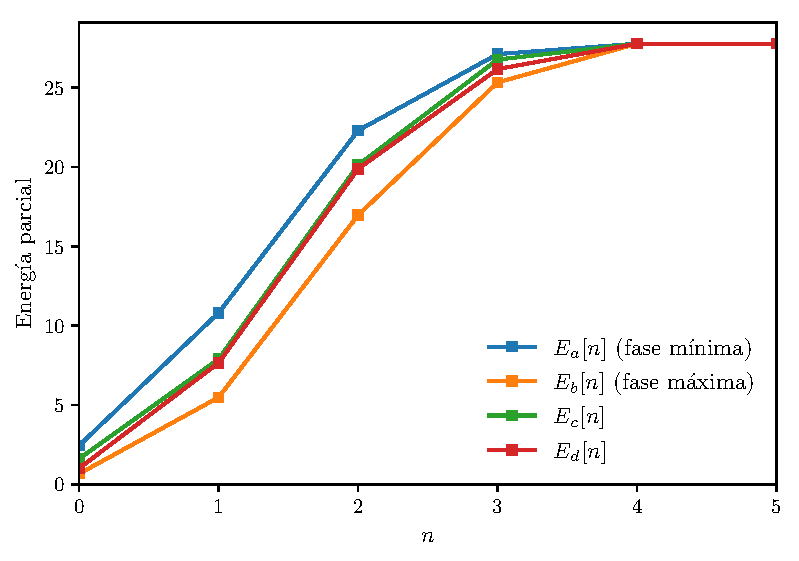
\includegraphics[width=0.76\textwidth]{figuras/example_5_13_minimum_energy_partial_energy.pdf}
 \caption{\label{fig:example_5_13_minimum_energy_partial_energy} Energía parcial de  las  cuatro secuencias de la figura \ref{fig:example_5_13_minimum_energy_impulse_responses}. El sistema de fase mínima produce el menor retardo de energía y el sistema de fase máxima produce el mayor retardo de energía.}
 \end{center}
\end{figure}

\section{Sistemas lineales con fase lineal generalizada}

En el diseño de sistemas de selección de frecuencias, es deseable lograr una magnitud de respuesta en frecuencia aproximadamente constante y fase nula en la banda pasante. Para sistemas causales, fase nula es inalcanzable, y por lo tanto, debe permitirse cierta distorsión de fase. Como se vio en la sección \ref{sec:transform_analysis_frequency_response_lti} el efecto de fase lineal con pendiente entera es un simple retardo temporal. Por otro lado, una fase no lineal puede alterar considerablemente la forma de la señal de entrada incluso cuando la magnitud de la respuesta en frecuencia es constante. En consecuencia, en muchas situaciones es importante el diseño de sistemas con fase exactamente o aproximadamente lineal. En esta sección se formalizan y generalizan las nociones de fase lineal y retardo ideal mediante la consideración de la clase de sistemas con retardo de grupo constante.

\subsection{Sistemas con fase lineal}\label{sec:transform_analysis_lineal_phase_systems}

Sea el sistema LTI cuya respuesta en frecuencia en un período es
\[
 H_\textrm{id}(e^{j\omega})=e^{-j\omega\alpha},
 \qquad\qquad 
 |\omega|<\pi,
\]
donde \(\alpha\) es un número real no necesariamente entero. Este sistema es un retardo ideal, donde \(\alpha\) es el retardo introducido por el sistema. Este sistema tiene repuesta en magnitud constante, fase lineal y retardo de grupo constante,
\[
 |H_\textrm{id}(e^{j\omega})|=1,
 \qquad\qquad 
 \angle H_\textrm{id}(e^{j\omega})=-\omega\alpha,
 \qquad\qquad
 \grd[H_\textrm{id}(e^{j\omega})]=\alpha. 
\]
La transformada inversa de Fourier de \(H_\textrm{id}(e^{j\omega})\) es la respuesta al impulso
\begin{equation}\label{eq:transform_analysis_ideal_delay_impulse_response}
 h_\textrm{id}[n]=\frac{\sen\pi(n-\alpha)}{\pi(n-\alpha)},
 \qquad\qquad 
 -\infty<n<\infty. 
\end{equation}
La salida de este sistema cuando la entrada es \(x[n]\) es
\[
 y[n]=x[n]*\frac{\sen\pi(n-\alpha)}{\pi(n-\alpha)}=\sum_{k=-\infty}^\infty x[k]*\frac{\sen\pi(n-k-\alpha)}{\pi(n-k-\alpha)}.
\]
Si \(\alpha=n_d\), donde \(n_d\) es un numero entero,
\[
 h_\textrm{id}[n]=\delta[n-n_d]
\]
y la salida es
\[
 y[n]=x[n]*\delta[n-n_d]=x[n-n_d].
\]
Es decir, si \(\alpha=n_d\) entero el sistema con fase lineal y ganancia unidad simplemente desplaza \(n_d\) muestras a la señal. Si \(\alpha\) no es  entero también es un retardo que se interpreta como se indica en la sección 4.5 de \cite{oppenheim2009discrete} (ver en particular el ejemplo 4.7). Si \(\alpha\) es positivo se trata de un retardo temporal y si \(\alpha\) es negativo es un avance temporal.

Esta discusión también brinda una interpretación útil de la fase lineal cuando está asociada a una respuesta en magnitud no constante. Por ejemplo, considérese la respuesta en frecuencia con fase lineal mas general dada por
\[
 H(e^{j\omega})=|H(e^{j\omega})|e^{-j\omega\alpha},
  \qquad\qquad 
 |\omega|<\pi,
\]
\begin{figure}[!htb]
 \begin{minipage}[c]{0.42\textwidth}
  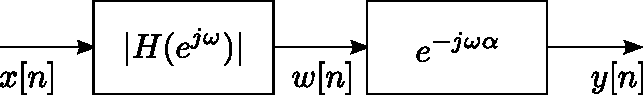
\includegraphics[width=\textwidth]{figuras/linear_phase_lti_system_cascade.pdf}
 \end{minipage}\hfill
 \begin{minipage}[c]{0.48\textwidth}
 \caption{representación de un sistema LTI de fase lineal como la casacada de un sistema de fase nula y un retardo temporal.
 }\label{fig:linear_phase_lti_system_cascade}
 \end{minipage}
\end{figure}
Esta ecuación sugiere la interpretación de la figura \ref{fig:linear_phase_lti_system_cascade}. La señal \(x[n]\) es filtrada por la respuesta en \(x[n]\) \(x[n]\) frecuencia de fase nula \(|H(e^{j\omega})|\) y la salida filtrada es desplazada temporalmente una cantidad \(\alpha\) entera o no entera. 
Supóngase por ejemplo que \(H(e^{j\omega})\) es el pasabajos ideal de fase lineal
\[
 H_\textrm{lp}(e^{j\omega})=
 \left\{
 \begin{array}{ll}
  e^{-j\omega\alpha}, &|\omega|<\omega_c,\\
  0,                  &\omega_c<|\omega|<\pi.
 \end{array}
 \right.
\]
La correspondiente respuesta al impulso es
\begin{equation}\label{eq:transform_analysis_ideal_lowpass_impulse_response}
 h_\textrm{lp}[n]=\frac{\sen\omega_c(n-\alpha)}{\pi(n-\alpha)}. 
\end{equation}
Observar que cuando \(\omega_c=\pi\) se obtiene la ecuación \ref{eq:transform_analysis_ideal_delay_impulse_response}.

\paragraph{Ejemplo: pasabajos ideal con fase lineal} La respuesta al impulso del pasabajos ideal ilustra algunas propiedades de los sistemas de fase lineal. Cuando \(\alpha=n_d\) es un entero, la respuesta en frecuencia es simétrica en torno a \(n=n_d\), es decir, se cumple que \(h_\textrm{lp}[n_d-n]=h_\textrm{lp}[n_d+n]\), o equivalentemente, \(h_\textrm{lp}[n]=h_\textrm{lp}[2n_d-n]\). Efectivamente,
\[
 h_\textrm{lp}[2n_d-n]=\frac{\sen\omega_c(2n_d-n-n_d)}{\pi(2n_d-n-n_d)}=\frac{\sen\omega_c(n_d-n)}{\pi(n_d-n)}
 =\frac{\sen\omega_c(n-n_d)}{\pi(n-n_d)}=h_\textrm{lp}[n].
\]
En este caso se puede definir un \emph{sistema de fase cero}
\[
 \hat{H}_\textrm{lp}(e^{j\omega})=H(e^{j\omega})e^{j\omega n_d}=|H(e^{j\omega})|,
\]
donde la respuesta es desplazada a la izquierda \(n_d\) muestras (si \(n_d>0\)) resultando en una secuencia par
\[
 \hat{h}_\textrm{lp}[n]=\frac{\sen\omega_c n}{\pi n}=\hat{h}_\textrm{lp}[-n].
\]
Otro caso a distinguir es cuando la pendiente \(\alpha\) de la fase lineal es un número entero mas un medio, o equivalentemente, \(2\alpha\) es entero. Puede mostrarse que también se cumple que 
\[
 h_\textrm{lp}[2\alpha-n]=h_\textrm{lp}[n].
\]
Observar que por ser \(2\alpha\) entero, el argumento \(2\alpha-n\) es entero por lo que \(h_\textrm{lp}[2\alpha-n]\) está bien definido. En este caso, el punto de simetría es \(\alpha\), que no es entero si no que es el punto medio entre dos muestras sucesivas. Como el punto de simetría no es un punto de la secuencia no es posible desplazar la secuencia para obtener una secuencia par. 
Un último tercer caso es cuando \(\alpha\) es un número real arbitrario, en donde la respuesta al impulso no tiene simetría. En ejemplo de cada caso se muestra en la figura \ref{fig:transform_analysis_example_05_14_linear_phase}.
\begin{figure}[!htb]
 \begin{center}
 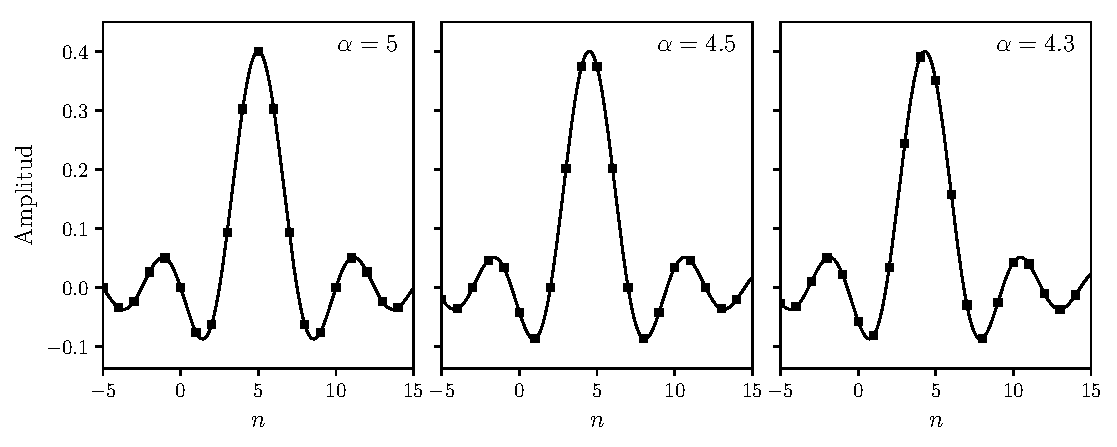
\includegraphics[width=1\textwidth]{figuras/transform_analysis_example_05_14_linear_phase.pdf}
 \caption{\label{fig:transform_analysis_example_05_14_linear_phase} Respuesta al impulso de pasabajos ideal con \(\omega_c=0.4\). Cuando \(\alpha=n_d\) es entero o \(2\alpha\) es entero, la respuesta al impulso es simétrica respecto a \(\alpha\), pero solo en el primer caso puede definirse un sistema de fase cer mediante un desplazamiento temporal. Cuando \(\alpha\) es un número real arbitrario no hay simetría.}
 \end{center}
\end{figure}

En general, un sistema de fase lineal tiene respuesta en frecuencia
\begin{equation}\label{eq:transform_analysis_lineal_phase_system_freq_response}
 H(e^{j\omega})=|H(e^{j\omega})|e^{-j\omega\alpha}. 
\end{equation}
Como se ilustró en el ejemplo, si \(2\alpha\) es un número entero, la respuesta al impulso tiene simetría par en torno a \(\alpha\), es decir,
\[
 h[2\alpha-n]=h[n].
\]
Si \(2\alpha\) no es entero, la respuesta al impulso no tiene simetría, pero igualmente el sistema tiene fase lineal o equivalentemente, retardo de grupo constante.

\subsection{Fase lineal generalizada}

En el caso de los sistemas con respuesta en frecuencia de la forma de la ecuación \ref{eq:transform_analysis_lineal_phase_system_freq_response}, la fase está completamente establecida por el factor de fase lineal \(e^{-j\omega\alpha}\) y es \(-\omega\alpha\). En consecuencia, los sistemas con respuesta en frecuencia de esa forma se llaman sistemas de fase lineal. Pero considérese por ejemplo el sistema de media móvil, cuya respuesta en frecuencia está dada por la ecuación \ref{eq:seq_and_sys_system_moving_average_causal_freq_response}. Esta respuesta en frecuencia consiste en una función real de \(\omega\) multiplicada por un factor de fase lineal pero no es estrictamente de fase lineal debido a los cambios de signo de la función real de \(\omega\), que contribuyen con saltos de \(\pi\) en la función de fase, como se muestra en la figura \ref{fig:example_02_16_moving_average_freq_response}. Notar que la fase en dicha figura no tiene saltos de \(2\pi\) por lo que es tanto el argumento principal como la fase desenrollada, es decir, el argumento principal de la fase y la fase desenrollada coinciden.

Muchas de las ventajas de los sistemas de fase lineal se aplican a los que tienen respuesta en frecuencia de la forma de la ecuación \ref{eq:seq_and_sys_system_moving_average_causal_freq_response} del sistema de media móvil, y en consecuencia es útil generalizar la definición del concepto de fase lineal. Específicamente, un sistema es referido como \emph{sistema de fase lineal generalizada} si su respuesta en frecuencia se puede expresarse como
\begin{equation}\label{eq:transform_analysis_generalizaed_lineal_phase_system_freq_response}
 H(e^{j\omega})=A(e^{j\omega})e^{-j\omega\alpha+j\beta}, 
\end{equation}
donde \(\alpha\) y \(\beta\) son constantes y \(A(e^{j\omega})\) es una función real de \(\omega\) que puede tomar tanto valores positivos como negativos. La fase de estos sistemas consiste en términos constantes sumados a la fase lineal \(-\omega\alpha\). Por lo tanto, la fase es una recta con discontinuidades producidas por la adición de los términos constantes, como en la figura \ref{fig:example_02_16_moving_average_freq_response}, y si se ignoran dichas discontinuidades, el sistema se caracteriza por tener un retardo de grupo constante. Es decir, la clase de sistemas tales que
\[
 \tau(\omega)=\grd[H(e^{j\omega})]=-\frac{d}{d\omega}\{\arg[H(e^{j\omega})]\}=\alpha
\]
tienen fase lineal de la forma mas general
\[
 \arg[H(e^{j\omega})]=\beta-\omega\alpha,
 \qquad\qquad
 0<\omega<\pi,
\]
donde \(\beta\) y \(\alpha\) son constantes.

En la sección \ref{sec:transform_analysis_lineal_phase_systems} se mostró que la respuesta al impulso de un sistemas con fase lineal tiene simetría en torno a \(\alpha\) si \(2\alpha\) es entero. Para ver la implicancia de esto para los sistemas de fase lineal generalizada se derivará una condición que debe ser satisfecha por \(h[n]\), \(\alpha\) y \(\beta\). Se parte notando que para dichos sistemas, la respuesta en frecuencia puede expresarse como
\begin{align*}
 H(e^{j\omega})&=A(e^{j\omega})e^{j(\beta-\omega\alpha)}\\
  &=A(e^{j\omega})\cos(\beta-\omega\alpha)+jA(e^{j\omega})\sen(\beta-\omega\alpha),
\end{align*}
o equivalentemente, como
\begin{align*}
 H(e^{j\omega})&=\sum_{n=-\infty}^\infty h[n]e{-j\omega n}\\
  &=\sum_{n=-\infty}^\infty h[n]\cos\omega n-j\sum_{n=-\infty}^\infty h[n]\sen\omega n,
\end{align*}
donde se asumió que \(h[n]\) es real. La tangente de la fase de \(H(e^{j\omega})\) puede expresarse como 
\[
 \tan(\beta-\omega\alpha)=\frac{\sen(\beta-\omega\alpha)}{\cos(\beta-\omega\alpha)}
  =\dfrac{-\displaystyle\sum_{n=-\infty}^\infty h[n]\sen\omega n}{\displaystyle\sum_{n=-\infty}^\infty h[n]\cos\omega n},
\]
por lo que la condición buscada es
\[
 \sen(\beta-\omega\alpha)\sum_{n=-\infty}^\infty h[n]\cos\omega n=-\cos(\beta-\omega\alpha)\sum_{n=-\infty}^\infty h[n]\sen\omega n,
\]
o equivalentemente,
\[
 \sum_{n=-\infty}^\infty h[n]\left\{\sen(\beta-\omega\alpha)\cos\omega n+\cos(\beta-\omega\alpha)\sen\omega n\right\}=0,
\]
y empleando la identidad trigonométrica \(\sin(x\pm y)=\sin x\cos y\pm\cos x\sin y\) resulta en que 
\begin{equation}\label{eq:transform_analysis_generalizaed_lineal_phase_general_condition}
 \sum_{n=-\infty}^\infty h[n]\sen[\omega(n-\alpha)+\beta]=0
 \qquad\textrm{para todo }\omega. 
\end{equation}
Esta ecuación establece una condición necesaria sobre \(h[n]\), \(\alpha\) y \(\beta\) para que el sistema tenga retardo de grupo constante. Sin embargo, no es una condición suficiente, y debido a su naturaleza implícita no indica como encontrar un sistema de fase lineal generalizada.

Una clase de sistemas de fase lineal generalizada son aquellos que cumplen que 
\begin{gather}
\begin{aligned}\label{eq:transform_analysis_generalizaed_lineal_phase_condition_symmetric}
  \beta&=0\quad\textrm{o}\quad\beta=\pi\\ 
  2\alpha&=M\;\textrm{entero}\\
  h[2\alpha-n]&=h[n]
\end{aligned}
\end{gather}
Con \(\beta=0\) o \(\beta=\pi\), la condición de la ecuación \ref{eq:transform_analysis_generalizaed_lineal_phase_general_condition} es
\begin{equation}\label{eq:transform_analysis_generalizaed_lineal_phase_condition_symmetric_sum}
  \sum_{n=-\infty}^\infty h[n]\sen[\omega(n-\alpha)]=0, 
\end{equation}
ya que en el caso en que \(\beta=\pi\) se cumple que \(\sen[\omega(n-\alpha)+\pi]=-\sen[\omega(n-\alpha)]\). Si \(2\alpha\) es un entero, los términos de la sumatoria \ref{eq:transform_analysis_generalizaed_lineal_phase_condition_symmetric_sum} pueden agruparse de a pares que se anulan para todo \(\omega\). Por ejemplo, si \(\alpha\) es entero, pueden agruparse las muestras equidistantes de la muestra de simetría \(\alpha\) como
\begin{align*}
 \sum_{n=-\infty}^\infty h[n]\sen[\omega(n-\alpha)]&=
  \sum_{n=-\infty}^{\alpha-1}\left\{h[n]\sen[\omega(n-\alpha)]+h[2\alpha-n]\sen[\omega(2\alpha-n-\alpha)]\right\}
  +h[\alpha]\sen0\\
  &=\sum_{n=-\infty}^{\alpha-1}\left\{h[n]\sen[\omega(n-\alpha)]-h[2\alpha-n]\sen[\omega(n-\alpha)]\right\}\\
  &=\sum_{n=-\infty}^{\alpha-1}(h[n]-h[2\alpha-n])\sen[\omega(n-\alpha)]\\
  &=0.
\end{align*}
En el caso en que \(\alpha\) es un número entero mas un medio, puede hacerse el razonamiento análogo, con el límite superior de la sumatoria siendo \(\alpha-1/2\).
Las condiciones \ref{eq:transform_analysis_generalizaed_lineal_phase_condition_symmetric} además implican que la respuesta en frecuencia \ref{eq:transform_analysis_generalizaed_lineal_phase_system_freq_response} es
\[
 H(e^{j\omega})=A(e^{j\omega})e^{-j\omega\alpha}e^{j\beta}
  \overset{(a)}{=}\pm A(e^{j\omega})(\cos\omega\alpha-j\sen\omega\alpha)
  =\pm A(e^{j\omega})\cos\omega\alpha\mp jA(e^{j\omega})\sen\omega\alpha,
\]
donde en \((a)\) se consideró que \(e^{j\beta}=\pm1\) con \(\beta=0\) o \(\beta=\pi\) respectivamente. Como si \(h[n]\) es real, \(H(e^{j\omega})\) tiene como parte real una función par y como parte imaginaria una función impar (ver la sección \ref{sec:seq_and_sys_dtft_symmetry_properties}), las condiciones \ref{eq:transform_analysis_generalizaed_lineal_phase_condition_symmetric} implican que \(A(e^{j\omega})\) es una función par.

Otra clase de sistemas de fase lineal generalizada son aquellos que cumplen que 
\begin{gather}
\begin{aligned}\label{eq:transform_analysis_generalizaed_lineal_phase_condition_antisymmetric}
  \beta&=\pi/2\quad\textrm{o}\quad\beta=3\pi/2\\ 
  2\alpha&=M\;\textrm{entero}\\
  h[2\alpha-n]&=-h[n]
\end{aligned}
\end{gather}
Esta vez la condición de la ecuación \ref{eq:transform_analysis_generalizaed_lineal_phase_general_condition} es
\begin{equation}\label{eq:transform_analysis_generalizaed_lineal_phase_condition_antisymmetric_sum}
  \sum_{n=-\infty}^\infty h[n]\cos[\omega(n-\alpha)]=0, 
\end{equation}
ya que \(\sen[\omega(n-\alpha)+\pi/2]=\cos[\omega(n-\alpha)]\) y \(\sen[\omega(n-\alpha)+3\pi/2]=-\cos[\omega(n-\alpha)]\), y se cumple para todo \(\omega\). Efectivamente, si por ejemplo \(\alpha\) es entero,
\begin{align*}
 \sum_{n=-\infty}^\infty h[n]\cos[\omega(n-\alpha)]&=\sum_{n=-\infty}^{\alpha-1}\left\{h[n]\cos[\omega(n-\alpha)]
  +h[2\alpha-n]\cos[\omega(2\alpha-n-\alpha)]\right\}+h[\alpha]\cos0\\
  &=\sum_{n=-\infty}^{\alpha-1}(h[n]+h[2\alpha-n])\cos[\omega(n-\alpha)]+h[\alpha]\\
  &=0.
\end{align*}
Observar que si \(\alpha\) es entero, la condición \(h[2\alpha-n]=-h[n]\) implica que \(h[\alpha]=0\). Además, la respuesta en frecuencia \ref{eq:transform_analysis_generalizaed_lineal_phase_system_freq_response} es
\[
 H(e^{j\omega})=A(e^{j\omega})e^{-j\omega\alpha}e^{j\beta}
  \overset{(a)}{=}\pm jA(e^{j\omega})(\cos\omega\alpha-j\sen\omega\alpha)
  =\pm A(e^{j\omega})\sen\omega\alpha\pm jA(e^{j\omega})\cos\omega\alpha,
\]
donde en \((a)\) se consideró que \(e^{j\beta}=\pm j\) con \(\beta=\pi/2\) y \(\beta=3\pi/2\) respectivamente. Esto implica que \(A(e^{j\omega})\) es una función impar ya que \(h[n]\) es real. 

Se concluye que las ecuaciones \ref{eq:transform_analysis_generalizaed_lineal_phase_condition_symmetric} y \ref{eq:transform_analysis_generalizaed_lineal_phase_condition_antisymmetric} brindan dos conjuntos de condiciones suficientes que garantizan fase lineal generalizada o retardo de grupo constante, pero también hay otros sistemas que cumplen la ecuación \ref{eq:transform_analysis_generalizaed_lineal_phase_system_freq_response} sin las condiciones de simetría, como el de la figura \ref{fig:transform_analysis_example_05_14_linear_phase} cuando \(2\alpha\) no es entero.

\subsection{Sistemas causales con fase lineal generalizada}

Causalidad y las condiciones de las ecuaciones \ref{eq:transform_analysis_generalizaed_lineal_phase_condition_symmetric} y \ref{eq:transform_analysis_generalizaed_lineal_phase_condition_antisymmetric} implica que 
\[
 h[n]=0,
 \qquad\qquad 
 n<0
 \qquad\qquad\textrm{y}\qquad\qquad
 n>M,
\]
es decir, sistemas FIR causales tienen fase lineal generalizada si tienen respuesta al impulso de largo \(M+1\) y satisfacen las condiciones de simetría en \ref{eq:transform_analysis_generalizaed_lineal_phase_condition_symmetric} o \ref{eq:transform_analysis_generalizaed_lineal_phase_condition_antisymmetric}. Específicamente, si
\begin{equation}\label{eq:transform_analysis_generalizaed_lineal_phase_fir_symmetric_impulse}
 h[n]=
 \left\{
 \begin{array}{ll}
  h[M-n],&0\leq n\leq M,\\
  0,&\textrm{en otro caso},
 \end{array}
 \right. 
\end{equation}
la respuesta en frecuencia es
\begin{equation}\label{eq:transform_analysis_generalizaed_lineal_phase_fir_symmetric_freq}
 H(e^{j\omega})=A_e(e^{j\omega})e^{-j\omega M/2}, 
\end{equation}
donde \(A_e(e^{j\omega})\) es una función real, par y periódica de \(\omega\). Análogamente, si
\begin{equation}\label{eq:transform_analysis_generalizaed_lineal_phase_fir_antisymmetric_impulse}
 h[n]=
 \left\{
 \begin{array}{ll}
  -h[M-n],&0\leq n\leq M,\\
  0,&\textrm{en otro caso},
 \end{array}
 \right. 
\end{equation}
la respuesta en frecuencia es
\begin{equation}\label{eq:transform_analysis_generalizaed_lineal_phase_fir_antisymmetric_freq}
 H(e^{j\omega})=jA_o(e^{j\omega})e^{-j\omega M/2}=jA_o(e^{j\omega})e^{-j\omega M/2+j\pi/2}, 
\end{equation}
donde \(A_e(e^{j\omega})\) es una función real, impar y periódica de \(\omega\).

Las condiciones \ref{eq:transform_analysis_generalizaed_lineal_phase_fir_symmetric_impulse} y \ref{eq:transform_analysis_generalizaed_lineal_phase_fir_antisymmetric_impulse} son suficientes para garantizar un sistema causal con fase lineal generalizada, pero no son condiciones necesarias. Es útil definir los siguientes cuatro tipos de sistemas FIR con fase lineal generalizada que se diferencian en el tipo de simetría y en si \(M\) es un número par o impar.

\paragraph{Sistema FIR de fase lineal tipo I} Un sistema tipo I tiene respuesta al impulso simétrica
como en la ecuación \ref{eq:transform_analysis_generalizaed_lineal_phase_fir_symmetric_impulse}
con \(M\) un número entero par. El retardo \(M/2\), que es el punto de simetría, es un entero. La respuesta en frecuencia es
\begin{align*}
 H(e^{j\omega})&=\sum_{n=0}^M h[n]e^{-j\omega n}\\
  &=\sum_{n=0}^{M/2-1}\left[h[n]e^{-j\omega n}+h[M-n]e^{-j\omega(M-n)}\right]+h[M/2]e^{-j\omega M/2}\\
  &\overset{(a)}{=}\sum_{n=0}^{M/2-1}h[n]e^{-j\omega M/2}\left[e^{-j\omega(n-M/2)}+e^{-j\omega(M/2-n)}\right]+h[M/2]e^{-j\omega M/2}\\
  &=e^{-j\omega M/2}\sum_{n=0}^{M/2-1}2h[n]\cos[\omega(M/2-n)]+h[M/2]e^{-j\omega M/2}\\
  &\overset{(b)}{=}e^{-j\omega M/2}\sum_{k=M/2}^1 2h[M/2-k]\cos\omega k+h[M/2]e^{-j\omega M/2},
\end{align*}
donde \((a)\) se empleó la condición de simetría y en \((b)\) se realizó el cambio de variable \(k=M/2-n\). La expresión resultante se puede escribir como
\[
 H(e^{j\omega})=e^{-j\omega M/2}\left(\sum_{k=0}^{M/2}a[k]\cos\omega k\right),
\]
donde
\begin{align*}
 a[0]&=h[M/2]\\
 a[k]&=2h[M/2-k],
 \qquad\qquad 
 k=1,\,2,\,\dots,\,M/2.
\end{align*}
Se observa que \(H(e^{j\omega})\) tiene la forma de la ecuación \ref{eq:transform_analysis_generalizaed_lineal_phase_fir_symmetric_freq}, y en particular, \(\beta\) en la ecuación \ref{eq:transform_analysis_generalizaed_lineal_phase_system_freq_response} es 0 o \(\pi\).

\paragraph{Sistema FIR de fase lineal tipo II} Un sistema tipo II tiene respuesta al impulso simétrica como en la ecuación \ref{eq:transform_analysis_generalizaed_lineal_phase_fir_symmetric_impulse}
con \(M\) un número entero impar. El punto de simetría \(M/2\) no es un entero si no que es un entero mas 1/2. La respuesta en frecuencia es
\begin{align*}
 H(e^{j\omega})&=\sum_{n=0}^M h[n]e^{-j\omega n}\\
  &=\sum_{n=0}^{(M-1)/2}\left[h[n]e^{-j\omega n}+h[M-n]e^{-j\omega(M-n)}\right]\\
  &\overset{(a)}{=}\sum_{n=0}^{(M-1)/2}h[n]e^{-j\omega M/2}\left[e^{-j\omega(n-M/2)}+e^{-j\omega(M/2-n)}\right]\\
  &=e^{-j\omega M/2}\sum_{n=0}^{(M-1)/2}2h[n]\cos[\omega(M/2-n)]\\
  &\overset{(b)}{=}e^{-j\omega M/2}\sum_{k=(M+1)/2}^1 2h[(M+1)/2-k]\cos[\omega(k-1/2)],
\end{align*}
donde \((a)\) se empleó la condición de simetría \ref{eq:transform_analysis_generalizaed_lineal_phase_fir_symmetric_impulse} y en \((b)\) se realizó el cambio de variable \(k=(M+1)/2-n\). La expresión se puede escribir como
\[
 H(e^{j\omega})=e^{-j\omega M/2}\left\{\sum_{k=1}^{(M+1)/2}b[k]\cos\left[\omega\left(k-\frac{1}{2}\right)\right]\right\},
\]
donde
\[
 b[k]=2h[(M+1)/2-k],
 \qquad\qquad 
 k=1,\,2,\,\dots,\,(M+1)/2.
\]
Nuevamente se observa que \(H(e^{j\omega})\) tiene la forma de la ecuación \ref{eq:transform_analysis_generalizaed_lineal_phase_fir_symmetric_freq}.

\paragraph{Sistema FIR de fase lineal tipo III} Si el sistema tiene respuesta al impulso antisimétrica
como en la ecuación \ref{eq:transform_analysis_generalizaed_lineal_phase_fir_antisymmetric_impulse}
con \(M\) un número entero par, puede mostrarse de forma análoga a como se hizo para el sistema de tipo I que la respuesta en frecuencia tiene la forma
\[
 H(e^{j\omega})=je^{-j\omega M/2}\left(\sum_{k=0}^{M/2}c[k]\sen\omega k\right),
\]
donde
\[
 c[k]=2h[M/2-k],
 \qquad\qquad 
 k=1,\,2,\,\dots,\,M/2.
\]
En este caso \(H(e^{j\omega})\) tiene la forma de la ecuación \ref{eq:transform_analysis_generalizaed_lineal_phase_fir_antisymmetric_freq}, y en particular, \(\beta\) en la ecuación \ref{eq:transform_analysis_generalizaed_lineal_phase_system_freq_response} es \(\pi/2\) o \(3\pi/2\).

\paragraph{Sistema FIR de fase lineal tipo IV} Si el sistema tiene respuesta al impulso antisimétrica como en la ecuación \ref{eq:transform_analysis_generalizaed_lineal_phase_fir_antisymmetric_impulse}
y \(M\) es un número entero impar, puede mostrarse igual que antes que la respuesta en frecuencia es
\[
 H(e^{j\omega})=je^{-j\omega M/2}\left\{\sum_{k=1}^{(M+1)/2}d[k]\sen\left[\omega\left(k-\frac{1}{2}\right)\right]\right\},
\]
donde
\[
 d[k]=2h[(M+1)/2-k],
 \qquad\qquad 
 k=1,\,2,\,\dots,\,(M+1)/2.
\]
Nuevamente se observa que \(H(e^{j\omega})\) tiene la forma de la ecuación \ref{eq:transform_analysis_generalizaed_lineal_phase_fir_antisymmetric_freq} y \(\beta\) en la ecuación \ref{eq:transform_analysis_generalizaed_lineal_phase_system_freq_response} es \(\pi/2\) o \(3\pi/2\). En la figura \ref{fig:transform_analysis_lineal_phase_fir_types} se muestra un ejemplo de respuesta al impulso de cada tipo de filtro FIR de fase lineal.
\begin{figure}[!htb]
 \begin{center}
 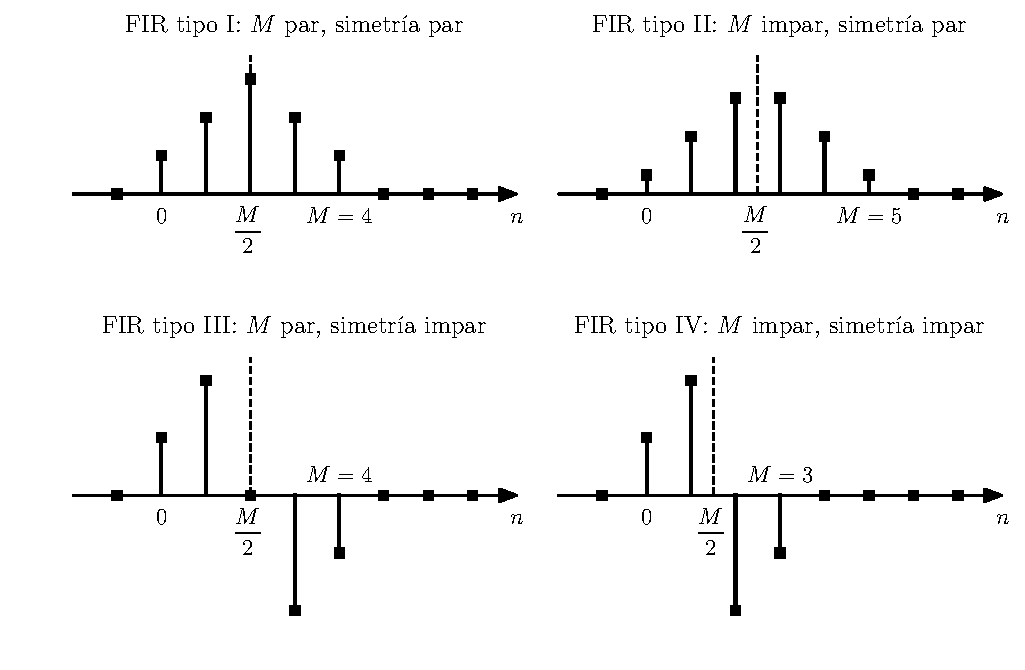
\includegraphics[width=0.9\textwidth]{figuras/transform_analysis_lineal_phase_fir_types.pdf}
 \caption{\label{fig:transform_analysis_lineal_phase_fir_types} Ejemplos de la respuesta al impulso de los cuatro tipos de filtros FIR de fase lineal.}
 \end{center}
\end{figure} 

\subsubsection{Ubicación de los ceros de los sistemas FIR de fase lineal}

Resulta instructivo considerar la ubicación de los ceros de los sistemas FIR de fase lineal. La función del sistema es
\[
 H(z)=\sum_{n=0}^M h[n]z^{-n}.
\]
En los casos en que la respuesta al impulso es simétrica (tipos I y II), se puede emplear la ecuación \ref{eq:transform_analysis_generalizaed_lineal_phase_fir_symmetric_impulse} para expresar \(H(z)\) como
\begin{equation}\label{eq:transform_analysis_lineal_phase_fir_types_zeros_locations_symmetric}
 H(z)=\sum_{n=0}^M h[M-n]z^{-n}=\sum_{k=M}^0 h[k]z^{k}z^{-M}=z^{-M}H(z^{-1}). 
\end{equation}
Esto indica que si \(z_0\) es un cero de \(H(z)\), se cumple que 
\[
 H(z_0)=z_0^{-M}H(z_0^{-1})=0,
\]
es decir, si \(z_0=re^{j\theta}\) es un cero de \(H(z)\), \(z_0^{-1}=r^{-1}e^{-j\theta}\) también es un cero de \(H(z)\). Además, si \(h[n]\) es real, los ceros deben estar en pares complejos conjugados, y por lo tanto \(z_0^*=re^{-j\theta}\) y \((z_0^*)^{-1}=r^{-1}e^{j\theta}\) también son ceros de \(H(z)\). Por lo tanto, si \(h[n]\) es real, cada cero complejo que no está en el círculo unidad será parte de un conjunto de cuatro ceros conjugados inversos de la forma 
\[
 (1-re^{j\theta}z^{-1})(1-re^{-j\theta}z^{-1})(1-r^{-1}e^{j\theta}z^{-1})(1-r^{-1}e^{-j\theta}z^{-1}).
\]
Si un cero de \(H(z)\) está en el círculo unidad, es decir, \(z_0=e^{j\theta}\), entonces \(z_0^{-1}=e^{-j\theta}=z_0^*\), lo que indica que los ceros sobre el círculo unidad están de a pares complejo conjugados,
\[
 (1-e^{j\theta}z^{-1})(1-e^{-j\theta}z^{-1}).
\]
Si un cero de \(H(z)\) es real y no está en el círculo unidad, el inverso también es un cero de \(H(z)\) y \(H(z)\) tendrá factores de la forma 
\[
 (1\pm rz^{-1})(1\pm r^{-1}z^{-1}).
\]
Finalmente, un cero de \(H(z)\) en \(z\pm1\) puede aparecer solo, ya que \(\pm1\) es su propio inverso y su propio conjugado. Por lo tanto, \(H(z)\) puede tener factores de la forma
\[
 (1\pm z^{-1}).
\]
El caso de un cero en \(z=-1\) es particularmente importante. De la ecuación \ref{eq:transform_analysis_lineal_phase_fir_types_zeros_locations_symmetric} se cumple que 
\[
 H(-1)=(-1)^MH(-1).
\]
Si \(M\) es par, esta ecuación es solo una simple identidad, pero si \(M\) es impar, \(H(-1)=-H(-1)\), lo que indica que \(H(-1)\) debe ser cero. Por lo tanto, en el caso de respuesta al impulso simétrica con \(M\) impar, la función del sistema debe tener un cero en \(z=-1\).

Si la respuesta al impulso es antisimétrica (tipos III y IV), el razonamiento análogo del que resultó la ecuación \ref{eq:transform_analysis_lineal_phase_fir_types_zeros_locations_symmetric} conduce en este caso a que 
\begin{equation}\label{eq:transform_analysis_lineal_phase_fir_types_zeros_locations_antisymmetric}
 H(z)=-z^{-M}H(z^{-1}). 
\end{equation}
Esta ecuación puede emplearse para mostrar que los ceros de \(H(z)\) en el caso antisimétrico están restringidos de la misma forma que los ceros en el caso simétrico. Sin embargo, en el caso antisimétrico son de especial interés tanto \(z=1\) como \(z=-1\). Con \(z=1\), la ecuación \ref{eq:transform_analysis_lineal_phase_fir_types_zeros_locations_antisymmetric} es
\[
 H(1)=-H(1).
\]
Por lo tanto, \(H(z)\) debe tener un cero en \(z=1\) para \(M\) par o impar. Con \(z=-1\), la ecuación \ref{eq:transform_analysis_lineal_phase_fir_types_zeros_locations_antisymmetric} es
\[
 H(-1)=(-1)^{-M+1}H(-1).
\]
En este caso, si \(M-1\) es impar, \(H(-1)=-H(-1)\). Por lo tanto, \(z=-1\) debe ser un cero de \(H(z)\) cuando \(M\) es par.

En la figura \ref{fig:transform_analysis_lineal_phase_fir_types_freq_responses} se muestra la magnitud de la respuesta en frecuencia de los cuatro tipos de filtros FIR de la figura \ref{fig:transform_analysis_lineal_phase_fir_types}. Se observa que cuando la repuesta al impulso es simétrica y \(M\) es impar (tipo II), la respuesta en frecuencia se anula en \(\omega=\pi\), acorde al hecho de que la función del sistema tiene un cero en \(z=-1\). En el caso en que la respuesta al impulso es antisimétrica se observa que la respuesta en frecuencia se anula en \(\omega=0\) y \(\omega=\pi\) si \(M\) es par (tipo III), ya que la función del sistema tiene ceros en \(z=\pm1\), y si \(M\) es impar (tipo IV), la respuesta en frecuencia se anula en \(\omega=\pi\) acorde al hecho de la función del sistema tiene un cero en \(z=-1\).
Estas restricciones en los ceros son importantes en el diseño de filtros FIR de fase lineal, ya que imponen limitaciones sobre los tipos de respuesta en frecuencia que pueden obtenerse. Por ejemplo, si se quiere aproximar un filtro pasa alto empleando una respuesta al impulso simétrica, \(M\) no puede ser impar, ya que la respuesta en frecuencia está restringida a ser nula en \(\omega=\pi\).
\begin{figure}[!htb]
 \begin{center}
 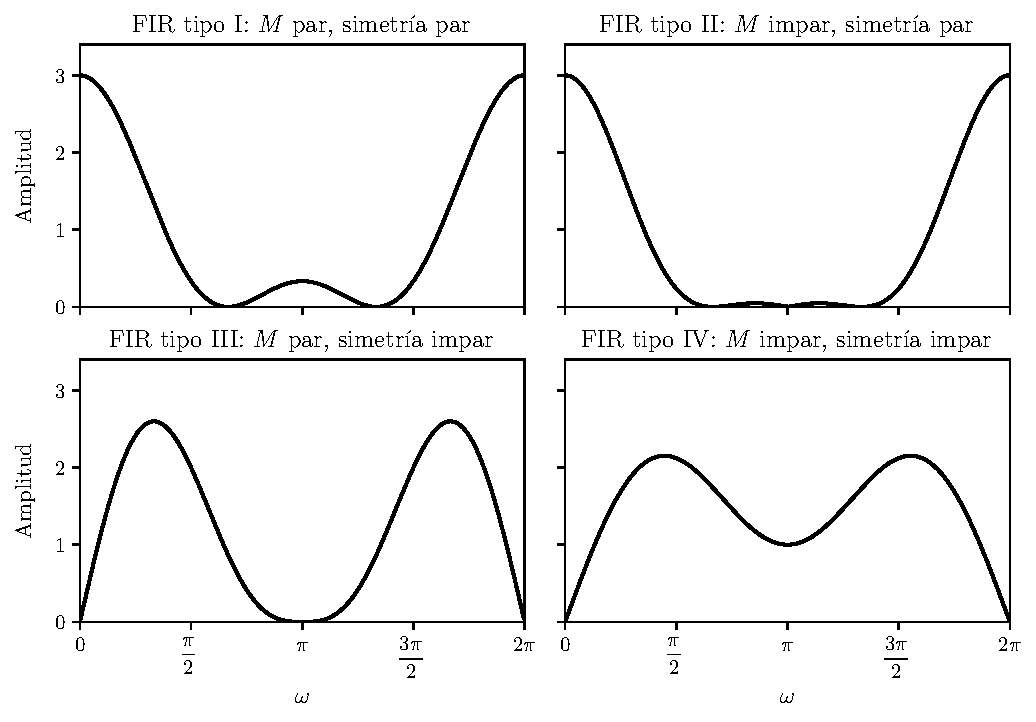
\includegraphics[width=0.9\textwidth]{figuras/transform_analysis_lineal_phase_fir_types_freq_responses.pdf}
 \caption{\label{fig:transform_analysis_lineal_phase_fir_types_freq_responses} Ejemplos de la magnitud de la respuesta en frecuencia de los cuatro tipos de filtros FIR de fase lineal. En todos los casos la fase el lineal con a lo sumo saltos de \(\pi\) radianes y el retardo de grupo es \(\alpha=M/2\) muestras constante.}
 \end{center}
\end{figure} 

\subsection{Relación entre sistemas FIR de fase lineal y sistemas de fase mínima}

En la discusión previa se mostró que los sistemas FIR de fase lineal con respuesta al impulso real tienen ceros sobre el círculo unidad o en posiciones conjugadas inversas. Por lo tanto, la función del sistema de un sistema FIR de fase lineal puede factorizarse en la cascada de un sistema de fase mínima \(H_\textrm{min}(z)\), un sistema de fase máxima \(H_\textrm{max}(z)\) y un sistema \(H_\textrm{uc}(z)\) que contiene ceros únicamente sobre el círculo unidad, es decir,
\begin{equation}\label{eq:transform_analysis_lineal_phase_fir_minimun_maximum_factorization_1}
 H(z)=H_\textrm{min}(z)H_\textrm{uc}(z)H_\textrm{max}(z) 
\end{equation}
donde
\begin{equation}\label{eq:transform_analysis_lineal_phase_fir_minimun_maximum_factorization_2}
 H_\textrm{max}(z)=H_\textrm{min}(z^{-1})z^{-M_i}, 
\end{equation}
y \(M_i\) es la cantidad de ceros de \(H_\textrm{min}(z)\). En la ecuación \ref{eq:transform_analysis_lineal_phase_fir_minimun_maximum_factorization_1}, \(H_\textrm{min}(z)\) tiene todos sus \(M_i\) ceros dentro del círculo unidad, \(H_\textrm{uc}(z)\) tiene todos sus \(M_o\) ceros sobre el círculo unidad. \(H_\textrm{max}(z)\) tiene todos sus \(M_i\) ceros fuera del círculo unidad, y de la ecuación \ref{eq:transform_analysis_lineal_phase_fir_minimun_maximum_factorization_2}, sus ceros son los inversos de los \(M_i\) ceros de \(H_\textrm{min}(z)\). El orden de la función del sistema \(H(z)\) es entonces \(2M_i+M_o\).

\paragraph{Ejemplo: descomposición de un sistema de fase lineal} Como ejemplo del uso de las ecuaciones \ref{eq:transform_analysis_lineal_phase_fir_minimun_maximum_factorization_1} y \ref{eq:transform_analysis_lineal_phase_fir_minimun_maximum_factorization_2}, considérese el sistema de fase mínima dado por la ecuación \ref{eq:transform_analysis_example_5_13_H_min},
\[
 H_\textrm{min}(z)=(1.25)^2(1-0.9e^{j0.6\pi}z^{-1})(1-0.9e^{-j0.6\pi}z^{-1})(1-0.8e^{j0.8\pi}z^{-1})(1-0.8e^{-j0.8\pi}z^{-1}).
\]
El sistema de fase máxima obtenido al aplicar la ecuación \ref{eq:transform_analysis_lineal_phase_fir_minimun_maximum_factorization_2} es
\begin{align*}
  H_\textrm{max}(z)&=(1.25)^2(1-0.9e^{j0.6\pi}z)(1-0.9e^{-j0.6\pi}z)(1-0.8e^{j0.8\pi}z)(1-0.8e^{-j0.8\pi}z)z^{-4}\\
   &=(1.25)^2(z^{-1}-0.9e^{j0.6\pi})(z^{-1}-0.9e^{-j0.6\pi})(z^{-1}-0.8e^{j0.8\pi})(z^{-1}-0.8e^{-j0.8\pi})\\
   &=(1.25)^2(0.9)^2(0.8)^2(1-1.1111e^{-j0.6\pi}z^{-1})(1-1.1111e^{j0.6\pi}z^{-1})\\
   &\qquad\times(1-1.25e^{-j0.8\pi}z^{-1})(1-1.25e^{j0.8\pi}z^{-1}),
\end{align*}
resultando en
\[
 H_\textrm{max}(z)=(0.9)^2(1-1.1111e^{j0.6\pi}z^{-1})(1-1.1111e^{-j0.6\pi}z^{-1})(1-1.25e^{j0.8\pi}z^{-1})(1-1.25e^{-j0.8\pi}z^{-1}),
\]
Si estos dos sistemas se colocan en cascada, por la ecuación \ref{eq:transform_analysis_lineal_phase_fir_minimun_maximum_factorization_2}, el sistema global
\[
 H(z)=H_\textrm{min}(z)H_\textrm{max}(z),
\]
tiene fase lineal. El diagrama de polos y ceros de los tres sistemas se muestra en la figura \ref{fig:example_05_19_zero_pole_plot}.
\begin{figure}[!htb]
 \begin{center}
 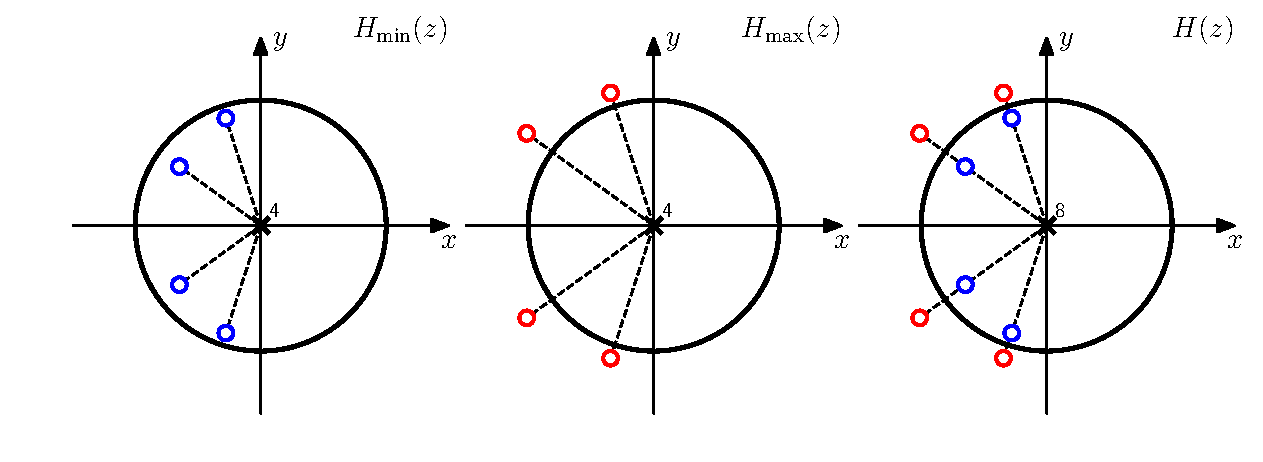
\includegraphics[width=0.97\textwidth]{figuras/example_05_19_zero_pole_plot.pdf}
 \caption{\label{fig:example_05_19_zero_pole_plot} Diagrama de polos y ceros diagrama de polos y ceros de los sistemas \(H_\textrm{min}(z)\), \(H_\textrm{max}(z)\) y \(H(z)\).}
 \end{center}
\end{figure}
Observar que por la ecuación \ref{eq:transform_analysis_lineal_phase_fir_minimun_maximum_factorization_2} y considerando que la respuesta al impulso es real,
\[
 H_\textrm{max}(e^{j\omega})=H_\textrm{min}(e^{-j\omega})e^{-j\omega M_i}=H^*_\textrm{min}(e^{j\omega})e^{-j\omega M_i}
\]
y por lo tanto,
\[
 |H_\textrm{max}(e^{j\omega})|=|H_\textrm{min}(e^{j\omega})|
 \qquad\qquad\textrm{y}\qquad\qquad
 \angle H_\textrm{max}(e^{j\omega})=-\angle H_\textrm{min}(e^{j\omega})-\omega M_i.
\]
La respuesta en frecuencia del sistema global se obtiene sumando la magnitud logarítmica, la fase y el retardo de grupo de los sistemas individuales. De esta forma,
\begin{align*}
 20\log_{10}|H(e^{j\omega})|&=20\log_{10}|H_\textrm{min}(e^{j\omega})|+20\log_{10}|H_\textrm{max}(e^{j\omega})|\\
   &=40\log_{10}|H_\textrm{min}(e^{j\omega})|.
\end{align*}
Además,
\begin{align*}
 \angle H(e^{j\omega})&=\angle H_\textrm{min}(e^{j\omega})+\angle H_\textrm{max}(e^{j\omega})\\
   &=\angle H_\textrm{min}(e^{j\omega})-\angle H_\textrm{min}(e^{j\omega})-\omega M_i\\
   &=-\omega M_i,
\end{align*}
donde \(M_i=4\) es la cantidad de ceros de \(H_\textrm{min}(z)\). Por último, el retardo de grupo de los sistemas combinados es
\[
 \grd[H(e^{j\omega})]=M_i=4.
\]
En la figura \ref{fig:example_05_19_freq_responses} se muestra la respuesta en frecuencia de los tres sistemas.
\begin{figure}[!htb]
 \begin{center}
 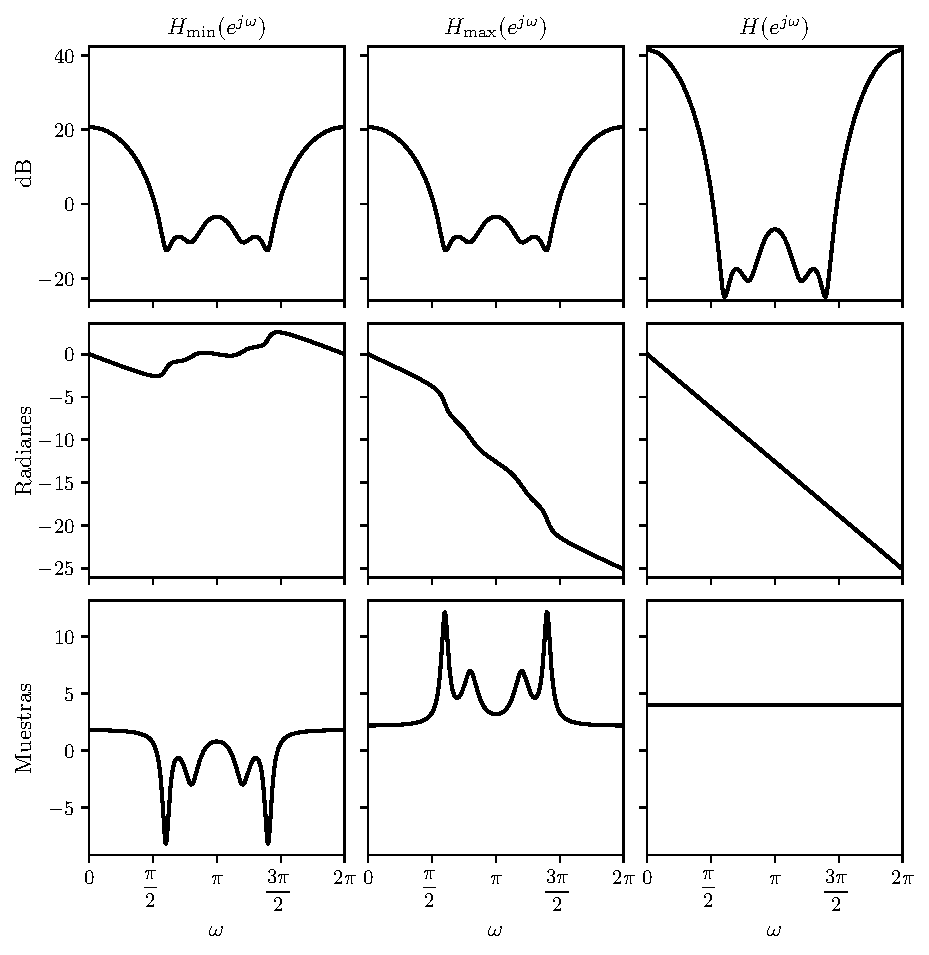
\includegraphics[width=0.97\textwidth]{figuras/example_05_19_freq_responses.pdf}
 \caption{\label{fig:example_05_19_freq_responses} Respuesta en magnitud logarítmica, la fase desenrollada y retardo de grupo de los sistemas \(H_\textrm{min}(z)\), \(H_\textrm{max}(z)\) y \(H(z)\).}
 \end{center}
\end{figure}






 

 
 
 
 
 

\bibliographystyle{ieeetr}
\bibliography{oppenheim_discrete_time}

\end{document}

